%\documentclass[preprint,12pt]{elsarticle}
\documentclass{article}

%!TEX root = THinstituteReport_1.tex

% Common file for including packages & definitions

%%%%%%%% PACKAGES %%%%%%%%
\usepackage[utf8]{inputenc}
\usepackage[T1]{fontenc}
\usepackage{amssymb}
\usepackage{amsmath}
\usepackage{graphicx}
\usepackage{epsfig,latexsym}
\usepackage{slashed}
\usepackage{geometry}
\geometry{a4paper, hmargin=2.5cm, vmargin=2.5cm}
\usepackage{simplewick}
%\usepackage{caption}
%\usepackage{subcaption}
\usepackage{nicefrac}
%\usepackage[colorlinks=true,linktocpage=true,linkcolor=blue,citecolor=blue]{hyperref}
\usepackage{hyperref}
\usepackage[dvipsnames]{xcolor}
\usepackage[normalem]{ulem}
\usepackage{url}
\usepackage[mathscr]{eucal}
%\usepackage{lineno}
%\linenumbers
\usepackage[affil-sl]{authblk}
%auth-sc

%\usepackage[doi=false,style=numeric-comp,citestyle=authoryear]{biblatex}
%%%%%%%% PACKAGES %%%%%%%%

%\addbibresource{THinstituteRefs.bib}
%\bibliography{THinstituteRefs.bib}

%\renewcommand\Authfont{\scshape\small}
\renewcommand\Authfont{\normalsize}
%\renewcommand\Affilfont{\itshape\small}
\renewcommand\Affilfont{\slshape\small}

\def\App#1{Appendix~\ref{#1}}
\def\sectionautorefname{Section\!}
\def\subsectionautorefname{Section\!}
\def\subsubsectionautorefname{Section\!}
\def\figureautorefname{Figure\!}
\def\tableautorefname{Table\!}

\newcommand{\gettitle}{Novel tools and observables for jet physics in heavy-ion collisions}
\hypersetup{
	colorlinks,
	linkcolor={blue},
	citecolor={blue},
	urlcolor={blue},
	%%%%%%%%%%%%%%%%%%%%%%%%%%%%%%%%%%
	pdftitle={\gettitle},
%	pdfauthor={},
	pdfkeywords={QCD jets} {Jet quenching} {Jet substructure}
	bookmarksopen=true,
	bookmarksopenlevel=2,
	bookmarksnumbered=true
}

%%%%%%%% DEFINITIONS %%%%%%%%
\def\be{\begin{eqnarray*}}
\def\ee{\end{eqnarray*}}
\def\beq{\begin{eqnarray}}
\def\eeq{\end{eqnarray}}
\def\bem{\begin{multline}}
\def\eem{\end{multline}}
\def\del{\partial}
\def\grad{\nabla}
\def\Eq#1{Eq.~(\ref{#1})}

\def\xperp{{x_\perp}}
\def\SL{{S(\lp,\lm)}}
\def\dfourk{\int\!\!\frac{\dd^4 k}{(2 \pi)^4}}
\def\dfourq{\int\!\!\frac{\dd^4 q}{(2 \pi)^4}}
\def\dfourkp{\int\!\!\frac{\dd^4 k'}{(2 \pi)^4}}
\def\dthreek{\int\!\!\frac{\dd^3 k}{(2 \pi)^3 2\omega_k}}
\def\dthreekp{\int\!\!\frac{\dd^3 k'}{(2 \pi)^3 2 \omega_{k'}}}
\def\dthreeq{\int\!\!\frac{\dd^3 q}{(2 \pi)^3 2\omega_q}}
\def\dthreeqp{\int\!\!\frac{\dd^3 q'}{(2 \pi)^3 2 \omega'}}
\def\dthreeqpm{\int\!\!\frac{\dd^3 q}{(q^+ + q^-)}}
\def\ddminqpm{\int\!\!\frac{\dd^{d-1} q}{(q^+ + q^-)}}
\def\MSbar{\overline{\small{\text{MS}}}}
\def\eps{0^+}
\def\vac{\text{vac}}
\def\med{\text{med}}
\def\gain{\text{gain}}
\def\loss{\text{loss}}
\def\coh{\text{coh}}
\def\incoh{\text{incoh}}
\def\tot{\text{tot}}
\def\cut{\text{cut}}
\def\virt{\text{virt}}
\def\jet{\text{jet}}
\def\dd{\text{d}}
\def\abar{\bar\alpha}
\def\QW{\text{\tiny QW}}
\def\BDMPS{\text{\tiny BDMPS}}
\def\thetajet{R}
\def\abar{\bar\alpha}
\def\soft{\text{soft}}
\def\alert#1{{\color{red}{#1}}}
\def\tdecoh{t_\text{d}}
\def\tform{t_\text{f}}

\newcommand{\onehalf}{{\nicefrac{1}{2}}}
\newcommand{\threehalfs}{{\nicefrac{3}{2}}}
\newcommand{\onefourth}{{\nicefrac{1}{4}}}
\newcommand{\onethird}{{\nicefrac{1}{3}}}
\newcommand{\sR}{{\rm \scriptscriptstyle{R}}}
\newcommand{\sL}{{\rm \scriptscriptstyle{L}}}
\newcommand{\sT}{{\rm \scriptstyle{T}}}
\newcommand{\sE}{{\rm \scriptscriptstyle{E}}}
\newcommand{\SK}{{\rm \scriptscriptstyle{SK}}}
\newcommand{\aPT}{a_{\rm \scriptscriptstyle{ PT}}}
\newcommand{\rme}{\text{e}}
\newcommand{\rmd}{\text{d}}
\newcommand{\kT}{k_{\text{\tiny T}}}
\newcommand{\pT}{p_{\text{\tiny T}}}
\newcommand{\pTzero}{p_{\text{\tiny T}(0)}}
\newcommand{\pTone}{p_{\text{\tiny T} 1}}
\newcommand{\pTtwo}{p_{\text{\tiny T} 2}}
\newcommand{\pTg}{p_\text{{\tiny T}g}}
\newcommand{\zg}{\ensuremath{z_\text{g}}}
\newcommand{\mg}{\ensuremath{M_\text{g}}}
\newcommand{\dr}{\ensuremath{\Delta R_\text{12}}}
\newcommand{\sst}{\scriptscriptstyle}

\def\pb{{\bar p}}
\def\pbp{{\bar p^+}}
\def\qm{{q^-}}
\def\qbp{{\bar q^+}}
\def\lp{{l^+}}
\def\lm{{l^-}}
\def\xp{{x^+}}
\def\xm{{x^-}}

\def\k{\boldsymbol{k}}
\def\q{\boldsymbol{q}}
\def\n{\boldsymbol{n}}
\def\x{\boldsymbol{x}}
\def\e{\boldsymbol{e}}
\def\p{\boldsymbol{p}}

\def\nn{\nonumber \\}
\def\Tebeb{T^{\bar e \bar e}}

\def\E{{\mathcal{E}}}
\def\O{{\mathcal{O}}}
\def\T{{\mathcal{T}}}
\def\P{{\mathcal{P}}}
\def\G{{\mathcal{G}}}
\def\A{{\mathcal{A}}}
\def\Xright{{\left| X_{us}\right\rangle}}
\def\Xleft{{\left\langle X_{us}\right|}}

\def\OL{{\mathbb{P}_\text{L}}}
\def\OR{{\mathbb{P}_\text{R}}}

\def\zcut{z_\text{cut}}
%%%%%%%% DEFINITIONS %%%%%%%%



%\journal{Physics Letters B} 

\begin{document}
\title{Novel tools and observables for jet physics in heavy-ion collisions}
%\large{Report of 5th Heavy Ion Jet Workshop/CERN TH institute, 25\textsuperscript{th} August-1\textsuperscript{st} September 2017}}
%
% \author[1]{Souvik Priyam Adhya}
% \author[1]{Harry Arthur Andrews}
% \author[1]{Liliana Apolinario}
% \author[1]{Francois Arleo}
% \author[1]{Austin Alan Baty}
% \author[1]{Redmer Alexander Bertens}
% \author[1]{Ran Bi}
% \author[1]{Christian Bierlich}
% \author[1]{Matteo Cacciari}
% \author[1]{Shanshan Cao}
% \author[1]{Jorge Casalderrey Solana}
% \author[1]{Wei Chen}
% \author[1]{Yi Chen}
% \author[1]{Yang-Ting Chien}
% \author[1]{Leticia Cunqueiro Mendez}
% \author[1]{Mrinal Dasgupta}
% \author[1]{Michal Deak}
% \author[1]{David d'Enterria}
% \author[1]{Fabio Dominguez}
% \author[1]{Rudiger Haake}
% \author[1]{Philip Coleman Harris}
% \author[1]{Hadi Hassan}
% \author[1]{Edmond Iancu}
% \author[1]{Peter Martin Jacobs}
% \author[1]{Kurt Jung}
% \author[1]{Krzysztof Kutak}
% \author[1]{Yen-Jie Lee}
% \author[1]{Tan Luo}
% \author[1]{Christopher Mc Ginn}
% \author[1]{Yacine Mehtar-Tani}
% \author[1]{Camelia Mironov}
% \author[1]{James Mulligan}
% \author[1]{Matthew Nguyen}
% \author[1]{Chang Ning-Bo}
% \author[1]{Cheng-Chieh Peng}
% \author[1]{Dennis Perepelitsa}
% \author[1]{Hendrik Poppenborg}
% \author[1]{Anton Rebhan}
% \author[1]{Rosi Jan Reed}
% \author[1]{Gunther Roland}
% \author[2]{Gavin Salam}
% \author[1]{Carlos A. Salgado}
% \author[1]{Dingyu Shao}
% \author[1]{Martin Spousta}
% \author[1]{Kaya Tatar}
% \author[1]{Guilherme Teixeira De Almeida Milhano}
% \author[2]{Konrad Tywoniuk}
% \author[1]{Marco Van Leeuwen}
% \author[1]{Marta Verweij}
% \author[1]{Victor Vila}
% \author[1]{Urs A. Wiedemann}
% \author[1]{Korinna C. Zapp}
% \author[1]{Nima Zardoshti}
%
% \affil[1]{please provide}
% \affil[2]{Theoretical Physics Department, CERN, 1211 Geneva 23, Switzerland}

\maketitle
%\newpage

\begin{abstract}
%\abstract{
Studies of fully reconstructed QCD jets in heavy-ion collisions remain one of the most firmly established programs aimed at extracting properties of hot and dense nuclear matter. Most recently, substructure observables have opened new and exciting directions by introducing techniques amenable to dissecting jets and extending the plethora of established observables. This report, summarizing the main lines of discussion at the 5th Heavy Ion Jet Workshop and CERN TH institute ``Novel tools and observables for jet physics in heavy-ion collisions'' in 2017, presents a first attempt at outlining a strategy for isolating and identifying the relevant physical processes that are responsible for the observed modifications by combining theory insights with sophisticated jet reconstruction techniques, including grooming and background subtraction algorithms. 
%}
\end{abstract}

\begin{flushright}
IFJPAN-IV-2018-8, MCNET-18-xx, CERN-TH-2018-xxx
\end{flushright}
%
%\tableofcontents

%!TEX root = THinstituteReport_1.tex

%%%%%%%%%%%%%%%%%%%%%%%%%%%%%%%%%%%%%%%%%%%%
\section{Introduction}
\label{sec:intro}
%%%%%%%%%%%%%%%%%%%%%%%%%%%%%%%%%%%%%%%%%%%%

%In recent years, observables involving fully reconstructed jets, produced in heavy-ion collisions, have been established as important tools to probe the properties of the underlying hot and dense QCD medium. From a reciprocal point of view, they also shed light on the details of parton fragmentation and hadronisation in the presence of final-state interactions. These developments are mainly driven by a dedicated experimental effort that aim at fully exploit the detector capabilities and experimental techniques at current high-energy colliders. On the theory side, an enhanced level of sophistication of the modeling of both jet fragmentation and its coupling to the medium evolution, often implemented as Monte-Carlo parton showers or event generators, allow to scrutinize the details of jet-medium interactions using a wide range of high-$\pT$ processes.
%
%Jets are excellent probes of the quark-gluon plasma (QGP) for several reasons; here we briefly outline but a few. Firstly, since they are multi-parton objects containing color degrees of freedom they are affected by final-state interactions with a deconfined medium. Secondly, in course of their evolution jets can probe various length scales of the QGP, providing a complementary window with regard to bulk observables that are dominated by soft physics.
%
%The way in which high-$\pT$ observables in heavy-ion collisions deviate from baseline measurements in proton-proton collisions is generically referred to as ``jet quenching''. This term arose historically in connection with the  first data on the suppression on high-$\pT$ hadron suppression and related di-jet/photon-jet asymmetries measured at RHIC. These processes clearly involve a large variety of scales, ranging from the jet scale to thermal scales of the QGP, as will also be explained in more detail below. Typical jet quenching observables will therefore be sensitive to perturbative and non-perturbative contributions in varying degree. This can complicate the interpretation of the considered observables and obfuscate the extraction of information about the underlying medium. Besides, additional background subtraction algorithms have to be applied in the more noisy heavy-ion environment, complicating the procedure of statistically removing detector effects (unfolding). Therefore a joint community effort between theory and experiment is crucial to fully take advantage of the potential of these QGP probes. 
%
%Many of these complications are less pressing or absent when measuring single-hadron spectra or hadron correlations. Hence, one notable example of such an joint effort was the so-called ``brick problem'' \cite{Armesto:2011ht,Burke:2013yra}, organized by the TECHQM collaboration \cite{TECHQM}, which aimed at clarifying differences and similarities between various theoretical implementations of jet quenching on the level of single-hadron spectra in heavy-ion collisions. The simplification allowing for such a comprehensive comparison was to reduce the complexity of the modeling of the underlying medium to a static, one-dimensional ``brick'' with constant density. 
%%While the employed models gave, as a result of comparison with the data, a wide spread of the obtained fundamental parameters, 
%Based on this exercise, it resulted in a comprehensive effort to estimate the jet quenching parameter $\hat q$ along with its uncertainties \cite{Burke:2013yra}.
%
%The joint organization of the 5th Heavy Ion Workshop and CERN TH institute ``Novel tools and observables for jet physics in heavy-ion collisions'' took place at CERN 25 August -- 1 September 2017 \cite{THinst}. The main objective of the meeting was to bring together experimentalists and theorists in order to identify relevant jet observables that are sensitive to different aspects of the final-state interactions with the dense medium created in heavy-ion collisions and study the added potential of jet substructure techniques in this context.
%
%Due to the high level of complexity related to the experimental determination and theoretical treatment of jet observables, a comprehensive effort of comparing models against each other and against data on a wide range of observables is out of  scope and, probably, would not allow to draw meaningful conclusions. Instead, the workshop provided an opportunity to consider jet observables in heavy-ion collisions from a new perspective to a large extent made available through novel substructure techniques.
%This report sums up the main discussions that took place during the meeting, and presents a selected number of numerical studies using existing tools. These mainly include the Monte Carlo (MC) event generators PYTHIA 8 \cite{Sjostrand:2007gs} for simulating the proton-proton baseline, and in-medium jet evolution codes QPYTHIA \cite{Armesto:2009fj} and JEWEL \cite{Zapp:2011ya,Zapp:2012ak}. 
%%{\color{red} Some details about main assumptions and building blocks of JEWEL and Q-PYTHIA. Appendix?}
%The selected parton shower MC's were used for sake of convenience, and we look forward to extend the suite of studied generators, including MARTINI \cite{Schenke:2009gb,Young:2011ug}, HYDJET++ \cite{Lokhtin:2008xi}, YaJEM \cite{Renk:2010zx} and MATTER \cite{Majumder:2013re} as well as newly developed codes, most notably JETSCAPE \cite{Cao:2017zih}, in future editions of the workshop. In addition, for jet reconstruction we made extensive use of FastJet \cite{Cacciari:2005hq,Cacciari:2011ma} and for the purposes of additional pile-up mitigation in heavy-ion context, we studied constituent subtraction (CS) \cite{Berta:2014eza} and SoftKiller (SK) \cite{Cacciari:2014gra}.
In heavy ion collisions at the LHC and at RHIC, essentially all hadronic high-$\pT$ observables deviate from baseline measurements in proton-proton collisions. The totality of these findings is generically referred to as ``jet-quenching''. It has been established first at RHIC on the level of single inclusive hadron spectra and high-$p_\perp$ hadron correlations. With the higher center of mass energies reached in nucleus-nucleus collisions at CERN's LHC, the focus has moved now to characterizing jet quenching in multi-hadron final states identified by modern jet finding algorithms.

There is overwhelming evidence that these jet quenching phenomena arise predominantly from final state interactions of the high-$\pT$-fragments of partonic scattering processes with the dense QCD matter produced in the collision region. Initial state effects such as nuclear modifications of parton distribution functions play a non-negligible but generally sub-dominant role. As a consequence, dynamical models of jet quenching focus mainly on the medium-induced modifications of final state parton showers. 

For the central aims of the relativistic heavy ion programmes at the LHC and at RHIC, jet quenching is of interest for at least two reasons. First, experimental access to information about the dense QCD matter produced in heavy ion collisions can be obtained from the scattering of calibrated hard probes on that matter. Second, since high-$\pT$-fragments are far-out-of-equilibrium, characterizing their medium-induced softening and isotropization may give access to the QCD equilibration processes and may thus help to understand whether, how and on which time scale heavy ion collisions evolve towards equilibrium. 

Jet quenching models, i.e., dynamical models of jet-medium interactions and the ensuing modifications of final state parton showers, are essential to 
infer from the measurements of quenched jets information about dense QCD matter and the equilibration processes that lead to it. Obviously, firm 
conclusions about QCD matter properties are only those that are independent of model-specific details, that are consistent with QCD theory and that are - within the range of validity of the dynamical model - consistent with the totality of experimental data. This necessitates the benchmarking of jet quenching models to establish where various models differ, and how experimental data can best discriminate between them.

With the aim of clarifying differences and similarities between various theoretical implementations of jet quenching on the level of single-hadron spectra, such a benchmarking exercise was organized by the TECHQM collaboration \cite{TECHQM}. For the success of this exercise, it was crucial to identify a simplified 
benchmark calculation that would allow for a comprehensive comparision since it could be easily preformed in all model set-ups. For the case of single inclusive
hadron spectra, this joint effort was the so-called ``brick problem'' \cite{Armesto:2011ht,Burke:2013yra},

From 21 August -- 1 September 2017 \cite{THinst}, the CERN TH Institute  {\it Novel tools and observables for jet physics in heavy-ion collisions} brought 
together at CERN 60 theorists and experimentalists with a research focus on jet quenching. The first three days of this two-week meeting were reserved 
to host the 5th in the series of {\it Heavy Ion Jet Workshops} {\bf REF}. 
Already in the preparatory phase of these meetings, the question arose how a TECHQM-like community 
effort could be extended from single-inclusive hadron spectra to medium-modified multi-particle final states. Within the first days of the meeting, {\bf the 
participants reached the consensus view that a comprehensive comparison of existing and future jet quenching models can be based on the
distribution of hadronic fragments in the Lund plane.} The focus of the ensuing discussion was two-fold. On the one hand, there was an effort to understand
how and for which dynamical reasons different the fragment distributions of different jet quenching models show marked differences. Second, there was an
effort to understand how modern jet substructure techniques can be utilized to focus on particular regions in the Lund plane, thus providing a possibility of
constructing jet observables that discriminate optimally between different models. 

This report summarizes the main strategy as formulated during the CERN TH Institute, and the subsequent studies on which the participants agreed. 
The main body of numerical results shown in this report are based 
on  the Monte Carlo (MC) event generators PYTHIA 8 \cite{Sjostrand:2007gs} for simulating the proton-proton baseline, and on the 
codes QPYTHIA \cite{Armesto:2009fj} and JEWEL \cite{Zapp:2011ya,Zapp:2012ak} for simulating in-medium jet evolution.
  For jet reconstruction we made extensive use of FastJet \cite{Cacciari:2005hq,Cacciari:2011ma} and for the purposes of additional pile-up mitigation in heavy-ion context, we explored constituent subtraction (CS) \cite{Berta:2014eza} and SoftKiller (SK) \cite{Cacciari:2014gra}. It would have been of obvious 
interest to include in this comparison on equal par other existing jet quenching Monte Carlos, such as MARTINI \cite{Schenke:2009gb,Young:2011ug}, HYDJET++ \cite{Lokhtin:2008xi}, YaJEM \cite{Renk:2010zx} and MATTER \cite{Majumder:2013re}. However, in the light of the committements of the workshop participants 
to contribute to this write-up, and on the timescale foreseen for this first exercise, such a comprehensive comparison was not possible. 
The numerical studies included in this report are therefore illustrative for the general strategy of jet model comparison as formulated at the workshop, 
but they are not comprehensive since they are based only on a small number of simulations done with a subset of all existing tools. In the coming years,
we  foresee the further development of existing jet quenching models, and the advent of new ones (such as those envisaged in the framework of 
JETSCAPE \cite{Cao:2017zih}). The main aim of this write-up is to formulate a simple, generally applicable strategy for characterizing differences
between jet quenching models and devising observables that allow one to discriminate best between them. The report is organized as follows:

 In \autoref{sec:phasespace}, we introduce for the first time, in the context of heavy-ion studies, the concept of a splitting map, based on the Lund kinematical diagram \cite{Andersson:1988gp}. Filling this map gives an operational representation of the radiation pattern implemented in a given showering algorithm. It also provides a direct, visual impression of what phase space region is being most significantly modified by medium effects. In detail, 
%We organize the report according to two main motifs. In the first part, \autoref{sec:phasespace}, we introduce for the first time, in the context of heavy-ion studies, the concept of a splitting map, based on the Lund kinematical diagram \cite{Andersson:1988gp}. Filling this map gives a operational representation of the radiation pattern implemented in a given showering algorithm. It also provides a direct, visual impression of what phase space region is being most significantly modified by medium effects. In detail, 
\begin{description}

\item[\autoref{sec:phasespace-theory}] gives a brief introduction to theoretical concepts that are useful for understanding the Lund diagram on the level of a single splitting, both for vacuum showers and showers in the medium.

\item[\autoref{sec:iterative-declustering}] describes in detail the procedure to fill the splitting map, by describing the steps related to jet reclustering and calculation of the variables that go into the map. 
%In particular, we study the impact of changing the reclustering algorithm, giving rise to different jet ``histories'' on the level of the PYTHIA vacuum shower. 

\item[\autoref{sec:phasespace-mc}] presents a study of the splitting maps of in-medium MC parton showers, QPYTHIA and JEWEL. 
We refer the interested reader to Appendix~\ref{app:models} for further details on the MC's utilized in the studies presented below. 
Finally, in \autoref{sec:uncorrelatedbackground}, we study the resilience of the observed   features at generator level to uncorrelated background by embedding the jet samples into a realistic heavy-ion environment.

\end{description}
While the splitting maps contain the maximal amount of information, since they accumulate the kinematics of every splitting, they are also amenable to more exclusive examinations for instance through the implementation of jet ``tagging'' and ``grooming'' procedures. These tools are extensively used in the high-energy community \cite{Bendavid:2018nar} for a wide range of purposes, spanning jet substructure studies and leveraging this control for studies of observables beyond pure QCD, see e.g. \cite{Larkoski:2017jix,Asquith:2018igt} for the most recent reviews. They have also been previously applied in Monte-Carlo studies for heavy-ion collisions \cite{Zhang:2015trf,Apolinario:2017qay,Milhano:2017nzm}. 
In studying concrete observables, we have mainly focussed on applying the so-called Soft Drop (SD) grooming procedure \cite{Larkoski:2014wba}, to be detailed below, that aims at identifying the first hard jet branching. 
Hence, in the second part of the report, \autoref{sec:jetsubstructure}, we perform a set of MC studies, on generator level and including embedding into a realistic heavy-ion background, using state-of-the-art grooming techniques. These observables are however, not limited to substructure but are also used in order to extract more differential aspects from inclusive jet observables. In detail, 
\begin{description}
\item[\autoref{sec:groomedobservables}] presents the result for the groomed momentum-fraction $z_g$, subjet angle $\Delta R_{12}$ and the groomed mass  $M_g$ for QPYTHIA and JEWEL using three grooming settings (in this section, the studies were performed on generator level). We shed more light on the robustness of these results by checking the size of hadronization effects in the $z_g$ distribution for three different SD settings \autoref{sec:hadronization}. As in \autoref{sec:iterative-declustering}, we also perform a brief study on how the reclustering algorithms modify the distributions.
\item[\autoref{sec:dissecting}] suggests a complementary look on substructure by submitting the jet sample that goes in to constructing a fully inclusive observable to an additional grooming step. Concretely, we propose to ``dissect'' the jet sample using SD grooming and bin the data in terms of the angular separation of the hardest subjets, $\Delta R_{12}$. We demonstrate this procedure on QPYTHIA and JEWEL samples for the nuclear modification factor $R_{AA}$ and the photon-jet imbalance.
\end{description}
Finally, we wrap up with an outlook in \autoref{sec:outlook}.



%Calculations of jet substructure \cite{Chien:2016led,Mehtar-Tani:2016aco,Milhano:2017nzm,Chang:2017gkt}, and data \cite{Sirunyan:2017bsd}.
%!TEX root = THinstituteReport_1.tex

%%%%%%%%%%%%%%%%%%%%%%%%%%%%%%%%%%%%%%%%%
%\section{Analysis of radiation phase space}
\section{Mapping the splittings of in-medium jets}
\label{sec:phasespace}
%%%%%%%%%%%%%%%%%%%%%%%%%%%%%%%%%%%%%%%%%


%%%%%%%%%%%%%%%%%%%%%%%%%%%%%%%%%%%%%%%%%
\subsection{Theoretical considerations}
\label{sec:phasespace-theory}
%%%%%%%%%%%%%%%%%%%%%%%%%%%%%%%%%%%%%%%%%


Jets are multi-particle observables and are experimentally accessed by assembling measured tracks and calorimeter energy deposition, or a combination of both, according to a jet algorithm. In the context of perturbative QCD, multiple splittings inside the jet cone have to be taken into account due to the mass singularity of QCD. 
In the medium, these splittings happen concurrently with, and are affected by, final-state interactions with the surrounding medium. It is therefore worth considering how medium scales, related to the medium size\footnote{For simplicity, in this section we treat the medium as static, where all jets traverse the same length $L$.} and the local properties, will have an impact on the phase space of jet observables. 

%%%%%%%%%%%%%%%%%%%%%%%%%%%%%%%%%%%%%
\begin{figure}
\centering
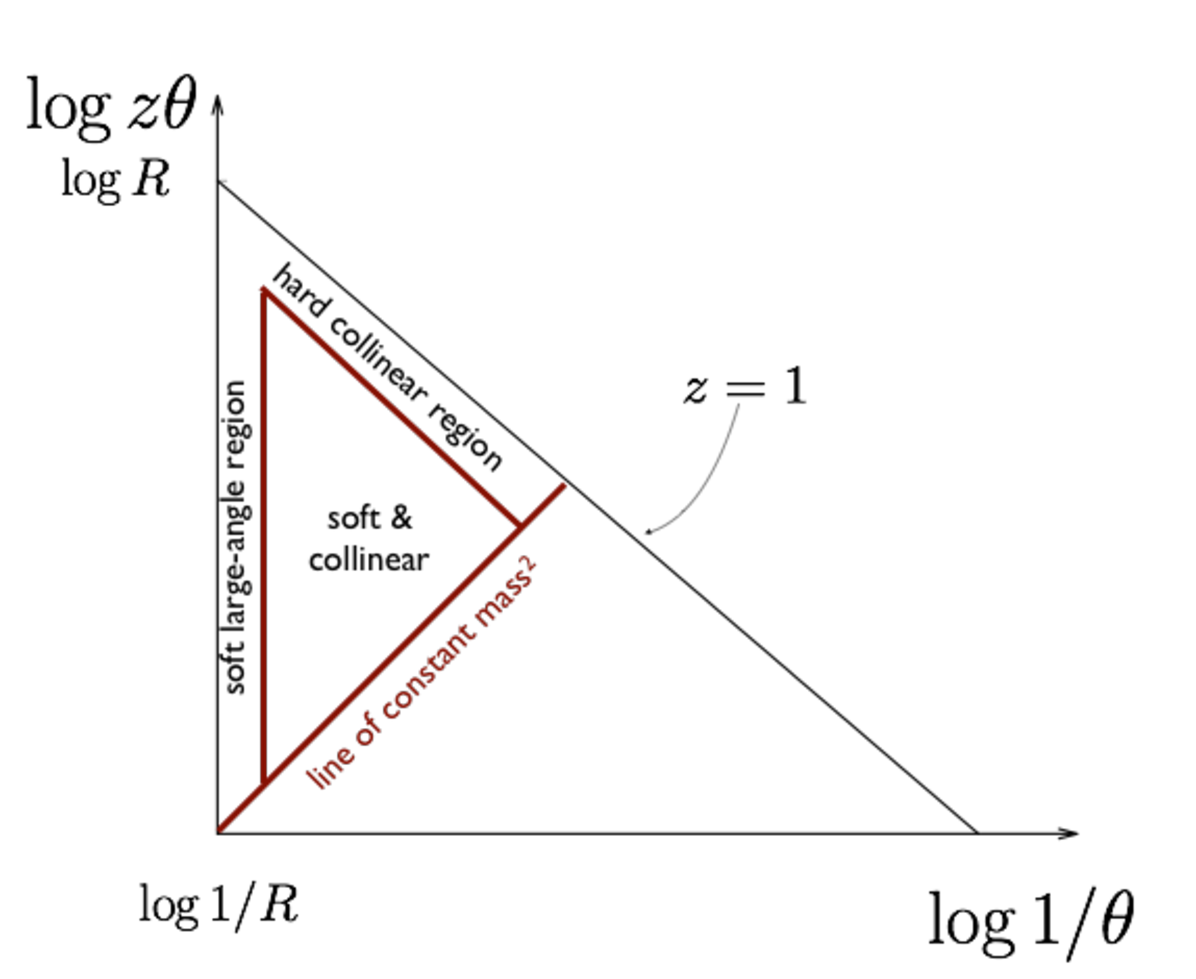
\includegraphics[width=0.6\textwidth]{figures/kinematics/lund_2}%
\caption{Lund kinematical diagram for vacuum radiation. Figure adapted from Ref.~\cite{Dasgupta:2013ihk}.}
\label{fig:PS0}
\end{figure}
%%%%%%%%%%%%%%%%%%%%%%%%%%%%%%%%%%%%%
In this context, it is very useful to introduce the Lund kinematical diagram \cite{Andersson:1988gp} for an arbitrary $1\to 2$ splitting process. In the soft and collinear limit, and in the absence of medium interactions, the differential probability $\dd P$ of emission of a gluon is given in terms of its kinematical variables by \cite{Dokshitzer:1991wu,Ellis:1991qj}
\beq
\label{eq:vacuum-phase-space}
\dd P = 2\frac{\alpha_s C_i}{\pi}\, \dd \log z\theta \, \dd \log\frac{1}{\theta} \,,
\eeq
where $z$ and $\theta$ are the momentum fraction and angle, respectively, of the gluon that is emitted off a projectile parton in arbitrary color representation ($C_i=C_F$ for quark and $C_i = N_c$ for gluon splitting, respectively). Hence, for fixed coupling, the area spanned below the line $z=1$, see \autoref{fig:PS0}, is uniformly populated by emissions with weight $2\alpha_s C_i/\pi$.
The radiation can take place up to the jet opening angle $R$.
In this figure we have also explicitly mapped out the regimes of soft, large-angle  and hard, collinear radiation. For future reference, it is worth keeping in mind that lines at fixed transverse momentum are horizontal, lines at fixed angle vertical, lines at fixed mass diagonal with a positive unit slope, and lines at fixed energy diagonal with a negative unit slope in this diagram. 

Before discussing any additional elastic or inelastic processes arising by the presence of a medium, one could consider the fate of vacuum emissions given a certain medium size. It can most naively be compared with the time it takes for a original parton to split into two daughter partons of invariant mass 
\beq
\label{eq:DipoleMass}
M^2 = z(1-z)\pT^2 \theta^2 \,,
\eeq
for small angles $\theta$, where $\pT$ is the longitudinal momentum of the parent parton, see Eq.~(\ref{eq:vacuum-phase-space}). This time is the so-called \textsl{formation time}, and is related to the uncertainty of the time-scale of splitting $\tform \sim \Delta E^{-1}$, and is explicitly given by
\beq
\label{eq:FormationTime}
\tform = \frac{2 z(1-z)\pT }{k_\perp^2} = \frac{2 \pT}{M^2} \,,
%(z \pT \theta^2)^{-1} \,,
\eeq
where $k_\perp = z(1-z)\pT \theta$, in the small angle limit, is the relative transverse momentum of the splitting. This formula can easily be understood as the time-scale for decaying in the rest frame of the parent times its boost factor $\sim (1/M) \times (\pT/M)$. In the following, we will only consider soft radiation and neglect and additional numerical factors to write $\tform \sim (z \pT \theta^2)^{-1} $.

Coming back to the diagram, let us identify emissions that happened inside the medium or, in other words, formation times that are shorter than the medium length ($\tform < L$). 
This condition results in an area on the Lund diagram delimited by the line solving $\tform = L$,
\beq
\log z \theta = \log \frac{1}{\theta} + \log \frac{1}{\pT L} \,,
\eeq
which is also represented in \autoref{fig:PS1}. Hence, the area above the line marked $\tform = L$ correspond to (vacuum) emissions that occur inside the medium. Emissions with $\tform > L$ occupy the region below the line.

In order to proceed, we will have to assume something about how the jet constituents interact with the medium. For illustrative purposes we will assume that all propagating particles experience diffusive momentum broadening, where the amount of accumulated momentum is characterized by the dispersion $\langle k_\perp^2 \rangle = \hat q t$, $t$ determining the time of in-medium propagation. The jet transport coefficient $\hat q$ acts as a diffusion constant in transverse space for the hard modes.\footnote{In this discussion, we neglect the influence of rare, hard kicks in the medium that go beyond this definition.} 
%While this reflects the expectation from multiple, soft interaction with a plasma and neglects rare, hard collisions, the latter can easily be incorporated into the same discussion.

%%%%%%%%%%%%%%%%%%%%%%%%%%%%%%%%%%%%%
\begin{figure}
\centering
%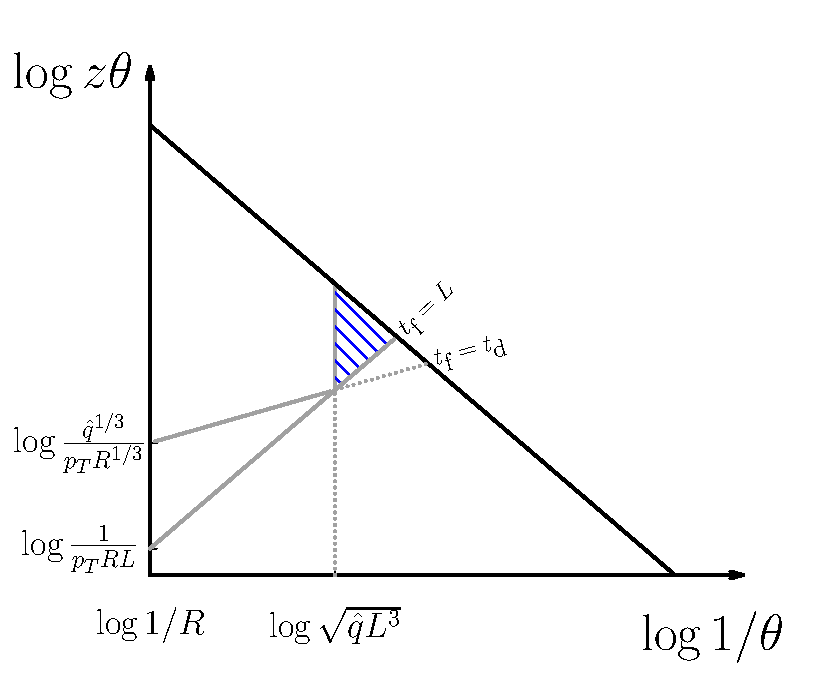
\includegraphics[width=0.5\textwidth]{figures/kinematics/plotVac}%
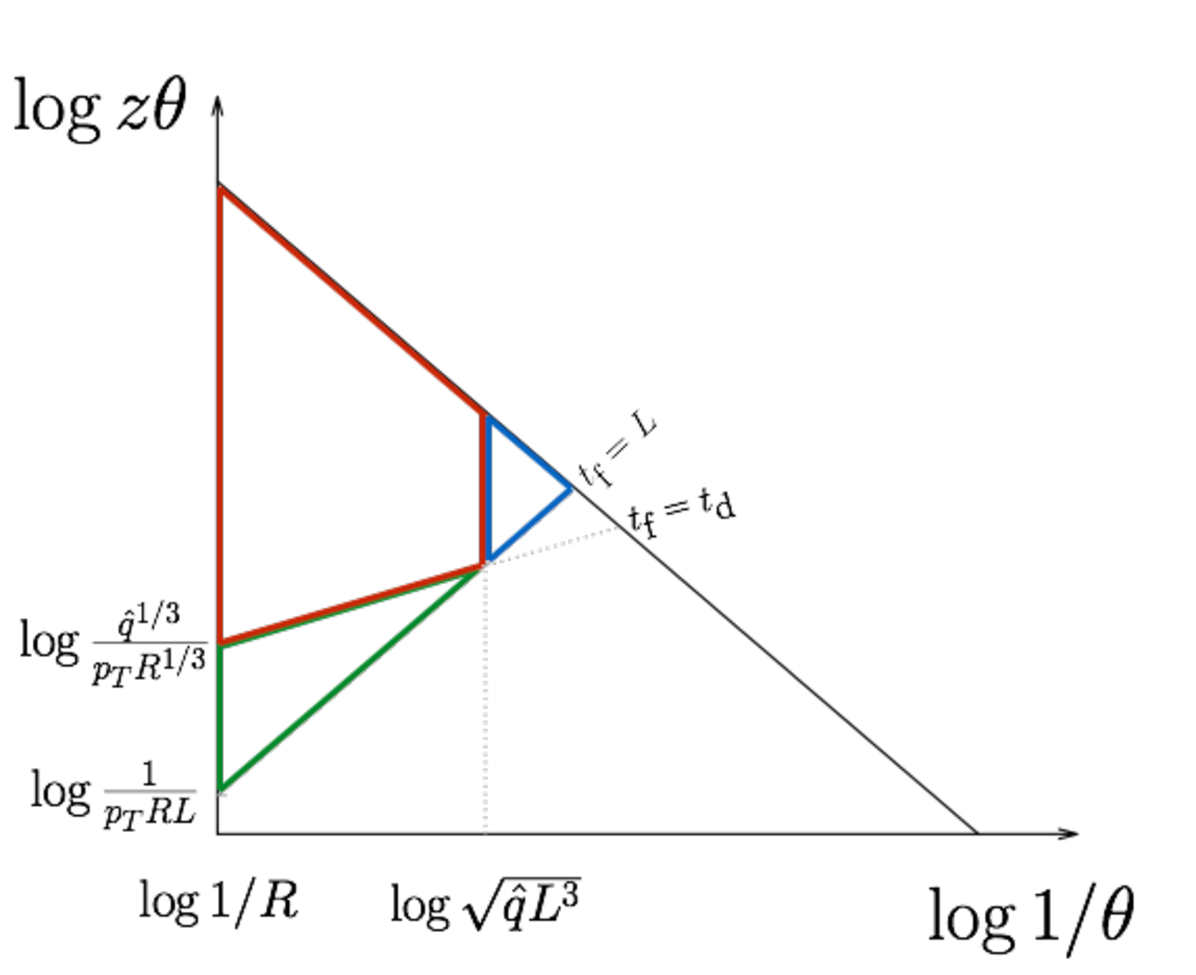
\includegraphics[width=0.6\textwidth]{figures/kinematics/lund_regions_colored}%
%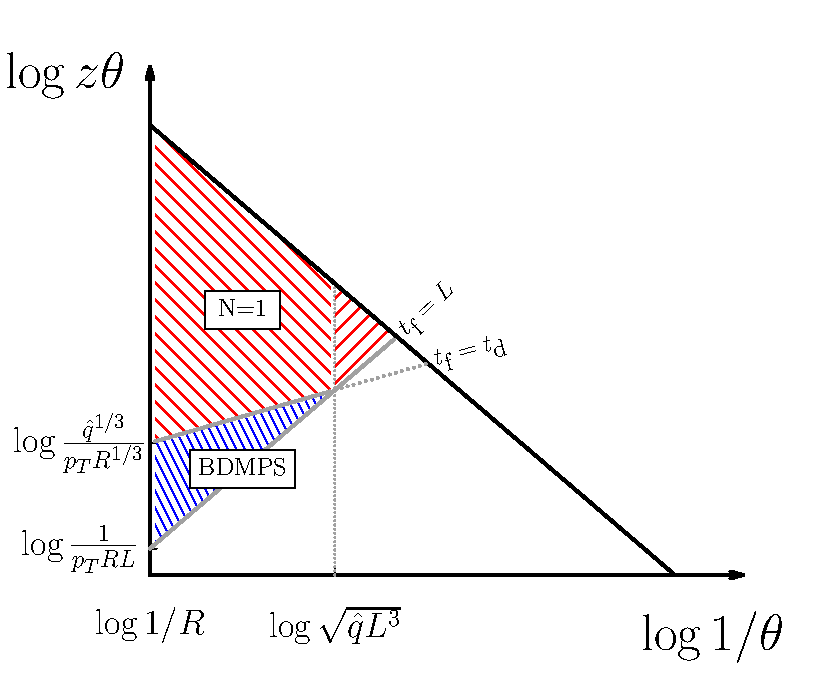
\includegraphics[width=0.5\textwidth]{figures/kinematics/plotMed}
\caption{Lund diagram for vacuum radiation with inclusion of relevant medium scales related to creation and decoherence of partons in the medium. The parameters are $\hat q = $ 2 GeV$^2$/fm, L = 2 fm and $p_{\scriptscriptstyle T}$ = 300 GeV. 
%Right: Lund diagram for medium induced radiation.
}
\label{fig:PS1}
\end{figure}
%%%%%%%%%%%%%%%%%%%%%%%%%%%%%%%%%%%%%
Having this picture in mind, a second time-scale immediately becomes relevant. It is typically referred to as the decoherence time, since it gauges whether medium interactions resolve a particular splitting. This occurs whenever the size of the pair, which can be estimated as $x_\perp \sim \theta t$ for small angles, becomes comparable to the medium resolution scale $\lambda_\perp \sim(\hat q t)^{-\onehalf}$ which in turn is inverse to the transverse momentum accumulated by multiple scattering.
By equating the two, $x_\perp \sim \lambda_\perp$, we find the parametric estimate for the decoherence time which turns out to be
\beq
\label{eq:DecoherenceTime}
\tdecoh = \left( \hat q \theta^2 \right)^{-\onethird} \,.
\eeq
Hence the line $\tform = \tdecoh$ is parameterized by
\beq
\log z\theta = \frac{1}{3} \log \frac{1}{\theta} + \log \frac{\hat q ^\onethird}{\pT} \,,
\eeq
and the area above this line represents the phase space for vacuum emissions.
As is clear from \autoref{fig:PS1}, this guarantees that at angles smaller than the minimal decoherence angle $\theta_c \sim (\hat q L^3)^{-\onehalf}$, the decoherence time is automatically larger than the medium length.\footnote{Since, $\tdecoh >L$ doesn't make much sense physically, we have represented this element by a dashed line in \autoref{fig:PS1}.} In particular, emissions with $\tform< \tdecoh < L$ correspond to pure vacuum splittings inside the medium that, during their subsequent propagation and possible further branching, will be resolved by medium interactions. Note also that the intersection point $\tform = \tdecoh$ corresponds to emissions with a transverse momentum scale $Q_s \sim(\hat q L)^{1/2}$ and the characteristic energy $\omega_c \sim \hat q L^2$.
The three time-scales we have identified -- the formation time, $\tform$, the decoherence time, $\tdecoh$, and the length of the medium, $L$ -- can be arranged in three possible orderings. These are marked out on \autoref{fig:PS1} as $\tform < \tdecoh < L $ by the red area, $\tform < L < \tdecoh$ by the blue area and $\tdecoh < \tform < L$ by the green area, respectively. 
%{\it The phase space of these regions is given by their area, and is easily found to be
%\begin{align}
%{\color{red} A_{\tform < \tdecoh < L}} &{\color{red}= \frac{1}{2}\ln \frac{R^2}{\theta_c^2} \left(\ln \frac{\pT}{\omega_c} + \frac{1}{3}\ln \frac{R^2}{\theta_c^2} \right)}  \,,\\
%{\color{blue} A_{\tform < L < \tdecoh}} &{\color{blue}= \frac{1}{4} \ln^2 \frac{\pT}{\omega_c}} \,,\\
%{\color{OliveGreen} A_{\tdecoh < \tform < L}} &{\color{OliveGreen}= \frac{1}{12} \ln^2 \frac{R^2}{\theta_c^2}} \,,
%\end{align}
%for $\pT > \omega_c$, where $\omega_c = \hat q L^2$.
%It is worth pointing out, that vacuum emissions that are emitted inside the medium at sufficiently small angles, $\theta < \theta_c$, remain unresolved by interactions with the medium \cite{MehtarTani:2010ma,MehtarTani:2011tz}. This implies that splittings in this region should follow a vacuum emission pattern, yet the jet is quenched (coherently) due to the presence of a total color charge \cite{CasalderreySolana:2012ef}. }
%It poses an exciting  challenge to pin this region down experimentally.
The second ordering is particularly interesting, giving rise to splittings that are formed inside the medium yet remain completely unresolved by medium interactions due to strong interference effects. It is often referred to as the coherence regime.

Before moving on, let us briefly contemplate a different model for the medium interactions. In this case, the resolution scale of the medium is simply the inverse of the medium momentum exchange, $\lambda_\perp \sim q_\perp^{-1}$. Now, the decoherence time is $\tdecoh \sim (\theta q_\perp)^{-1}$ which gives to a minimal coherence angle $\theta_c \sim (q_\perp L)^{-1}$. In effect, the coherence regime exists only for sufficiently soft interactions $q_\perp < \sqrt{\pT/L}$.

Now let us briefly review the possible additional radiative channels that are opened due to interactions with the medium. It is important to stress that the emission probability for medium-induced radiation, such as Eq.~(\ref{eq:vacuum-phase-space}) for the vacuum radiation, does not factorize in the same way. Hence, the phase space in the Lund diagram is not anymore uniformly filled. 

Let us firstly describe the multiple scattering regime. It applies to situations when, in course of their formation, induced gluons experience transverse momentum broadening, approximated by $\langle k_\perp^2 \rangle \lesssim \hat q \tform$, see e.g. \cite{Kurkela:2014tla} for a more thorough discussion. We can invert this relation to find that the formation time of the emitted particles becomes $\tform(\omega) \sim \sqrt{\omega/\hat q}$. 
Gluons with the longest formation time $\tform= L$, carry energy $\omega_c \sim \hat q L^2$.
%Reciprocally, $k_{\rm f}^2 \sim \sqrt{\hat q \omega}$ or, in terms of emission angle, $\theta_{\rm f}(\omega) \sim (\hat q/\omega^3)^{\onefourth}$. 
%The spectrum of emitted gluons per unit of energy is therefore
%\beq
%\label{eq:BDMPS-spectrum}
%\dd {\cal P}_{\rm med} = 2 \frac{\alpha_s C_{\tiny R}}{\pi} \frac{L}{\tform(\omega)}\frac{\dd \omega}{\omega} \,,
%\eeq
%for $\tform \ll L$ or, in other words, $\omega \ll \omega_c$, where $\omega_c \sim \hat q L^2$. 
This energy scale also acts as an effective cut-off scale, as for $\omega > \omega_c$ the spectrum is strongly suppressed (LPM suppression). It also determines a ``minimal'' angle for gluon emission due to multiple scattering, denoted $\theta_{\rm f}(\omega_c) \sim (\hat q L^3)^{-\onehalf}$, that we already encountered as a minimal angle for coherence in the discussion above.
%Hence, LPM radiation contributes maximally along the line $\tform \sim \tdecoh$. 
It involves formation times longer than the decoherence time $\tform \gtrsim \tdecoh$, which implies $k_{\rm f} \lesssim \sqrt{\hat q \omega}$, and angles $\theta > \theta_c$. Furthermore, the multiplicity of LPM gluons becomes large in the soft sector, in particular at $\omega \lesssim \alpha_s^2 \omega_c$. In this regime, resummation of multiple medium-induced gluons is necessary.

This medium-induced radiative component is expected to enhance the yield around $\tform \sim \tdecoh$. It is however worth keeping in mind that due to broadening and subsequent splitting, it is expected that these quanta will be effectively transported out of the jet cone. What remains is therefore a residual impact of ``energy loss'' that affects the vacuum like branchings inside the medium, see \autoref{sec:phasespace-mc} for results from in-medium Monte Carlo showers.

In addition to the (relatively) soft emissions that are sensitive to multiple scattering, there arises a radiative component from rare, hard kicks in the medium. This component is formally higher-twist, i.e. scales as $\sim k_\perp^{-4}$, and has to be induced inside the medium, $\tform < L$. It is however subleading to the the LPM emissions that dominate close to the line $\tform \sim \tdecoh$.
These emissions will typically not undergo further splittings and can contribute to the intra-jet distribution. 

To summarize, from perturbative arguments regarding medium-induced radiative processes we expect to observe large medium-effects in the region marked by green in \autoref{fig:PS1}, which overlaps with the region where LPM radiation is abundant. In the absence of medium interactions, the theoretical expectation is approximately reproduced by vacuum Monte Carlo showers, see \autoref{sec:iterative-declustering} for more details. In \autoref{sec:phasespace-mc} we compare our theoretical expectation with models that implement medium modifications. This concludes the physics discussion of possible radiative contributions at the level of single splitting. It is worth keeping in mind that what we have discussed so far is an idealized picture that will be complicated by the embedding the jets into correlated and un-correlated medium backgrounds. We have also neglected a set of other effects, such as medium back-reaction, that could possibly become important for realistic modeling of the jet-medium interactions.

%%%%%%%%%%%%%%%%%%%%%%%%%%%%%%%%%%%%%%%%
\subsection{Filling the map from reclustered of jets}
\label{sec:iterative-declustering}
%%%%%%%%%%%%%%%%%%%%%%%%%%%%%%%%%%%%%%%%

The generalization of this picture to multiple emissions is more delicate. In vacuum, subsequent emissions are self-similar (apart from the running of $\alpha_s$) which allows to iterate the splitting process with the jet opening angle R replaced by the splitting angle of the parent dipole (angular ordering) \cite{Dokshitzer:1991wu}. 

In order to connect theory with experimental observables, one relies on an operational definition of what a jet is. Such procedures cluster the final-state stable particles using sequential recombination algorithms, e.g. as implemented in FastJet \cite{Cacciari:2005hq,Cacciari:2011ma}. Final state particles $i$ and $j$ are assigned a mutual distance $d_{ij}$ and a distance to the beam $d_{i\rm B}$. The pair with the smallest distance are recombined first, and the algorithm repeats until the distance to the beam is the smallest quantity. In this case, the algorithm terminates labelling $i$ a jet. The distance metric is generally defined as
\begin{align}
\label{eq:JetDistanceMetric}
d_{ij} &= \min\left(p_{{\rm \tiny T},i}^{2\alpha},p_{{\rm \tiny T},j}^{2\alpha} \right) \frac{\Delta R_{ij}^2}{R^2} \,, \\
d_{i \rm B} &= p_{{\rm \tiny T},i}^{2\alpha} \,,
\end{align}
where $\Delta R_{ij}^2 = (\Delta \phi_{ij})^2 + (\Delta \eta_{ij})^2$ and $\alpha$ is a constant that defines the algortihm; $\Delta \phi_{ij}$ ($\Delta \eta_{ij}$) being the separation of the particles in azimuthal angle (pseudorapidity). In our studies, we have used the anti-$k_{\rm \tiny T}$ algorithm ($\alpha = -1$) \cite{Cacciari:2008gp}, the Cambridge/Aachen (C/A) algorithm ($\alpha = 0$) \cite{Dokshitzer:1997in,Wobisch:1998wt}, and the $k_{\rm \tiny T}$ algorithm ($\alpha = 1$) \cite{Catani:1993hr,Ellis:1993tq}.

Given a reconstructed jet, obtained from a full heavy-ion event, with a list of constituents belonging to it
%, or perhaps after including a stage of additional mitigation of unwanted background, 
one can repeat the recombination using one of the algorithms described above. In this context, this is referred to as a reclustering of the jet, providing a complete hierarchical tree (aka ``history'') of the jet evolution. Substructure techniques, to be used extensively throughout this report, define observables based on the information organized in such a tree. 
%Usually, one retraces the nodes of the tree in a stepwise fashion, in a process called declustering.
It is important to keep in mind that, depending on the reclustering algorithm, the information stored in the tree is only approximately related to the sequence of quark and gluon splittings that build the jet structure as understood within perturbative QCD. 
%In vacuum, the correspondence is most reliable for the C/A algorithm due to angular odering, but for medium showers, which comprise particles that are not angular ordered, other algorithms could potentially become relevant.

In order to extract relevant information from a sample of real (simulated) jets, we apply the following procedure.
%Uncovering this sequence of splittings should be in close correspondence to filling the Lund diagram using the following procedure. 
For a given jet in the sample, fill the Lund diagram by
\begin{description}
\item[1)] build a history of splittings by reclustering a jet with a given reclustering algorithm,
\item[2)] at each branching, extract the variables $z$ and $\theta$. Here, we define $z \equiv z_\text{rel} = p_{t,j_2}/(p_{t,j_1}+p_{t,j_2})$ and use $\log(z \Delta R_{j_1 j_2}/R)$ as the quantity on the $y$-axis, where $j_i$ ($i=1,2$) refer to two branches of the tree.
%\footnote{We thank G.~Salam for a discussion on this point.} 
This definition of $z$ has the property that it always reflects the momentum sharing within that  specific step.

\end{description}
%The Lund plane is thus populated for a sample of jets.
The C/A reclustering, where the distance metric is only determined by the angular separation, see Eq.~(\ref{eq:JetDistanceMetric}), should correspond most closely to a angular-ordered sequence of splittings based on our arguments above. That means that the last step of jet reclustering merges two substructures separated at large angles.
Alternative reclustering strategies can however be used, although it would distort the correspondence with showers that implement angular ordering. Given that we also will study other types of parton showers, e.g. that include medium effects, we have also studied the use of the (anti-)$k_{\rm \tiny T}$ algorithms in this step. 
%The strategy of the clustering algorithm manifests itself in the declustering and grooming. CA algorithm combines the closest particles first. As a consequence, the first declustering steps will encounter soft splittings at large angle. 
In the case of the $k_{\rm \tiny T}$-algorithm, the softest particles are clustered first. As a consequence, the last reclustering step will merge hard splittings. The anti-$k_{\rm \tiny T}$ clusters hard particles first, thus splittings at the last reclustering steps will be generally soft. 
%Such ordering is reflected in the Lund plots of \autoref{fig:AlgoDependence}.


%%%%%%%%%%%%%%%%%%%%%%%%%%%%%%%%%%%%%
\begin{figure}[t!]
\centering
%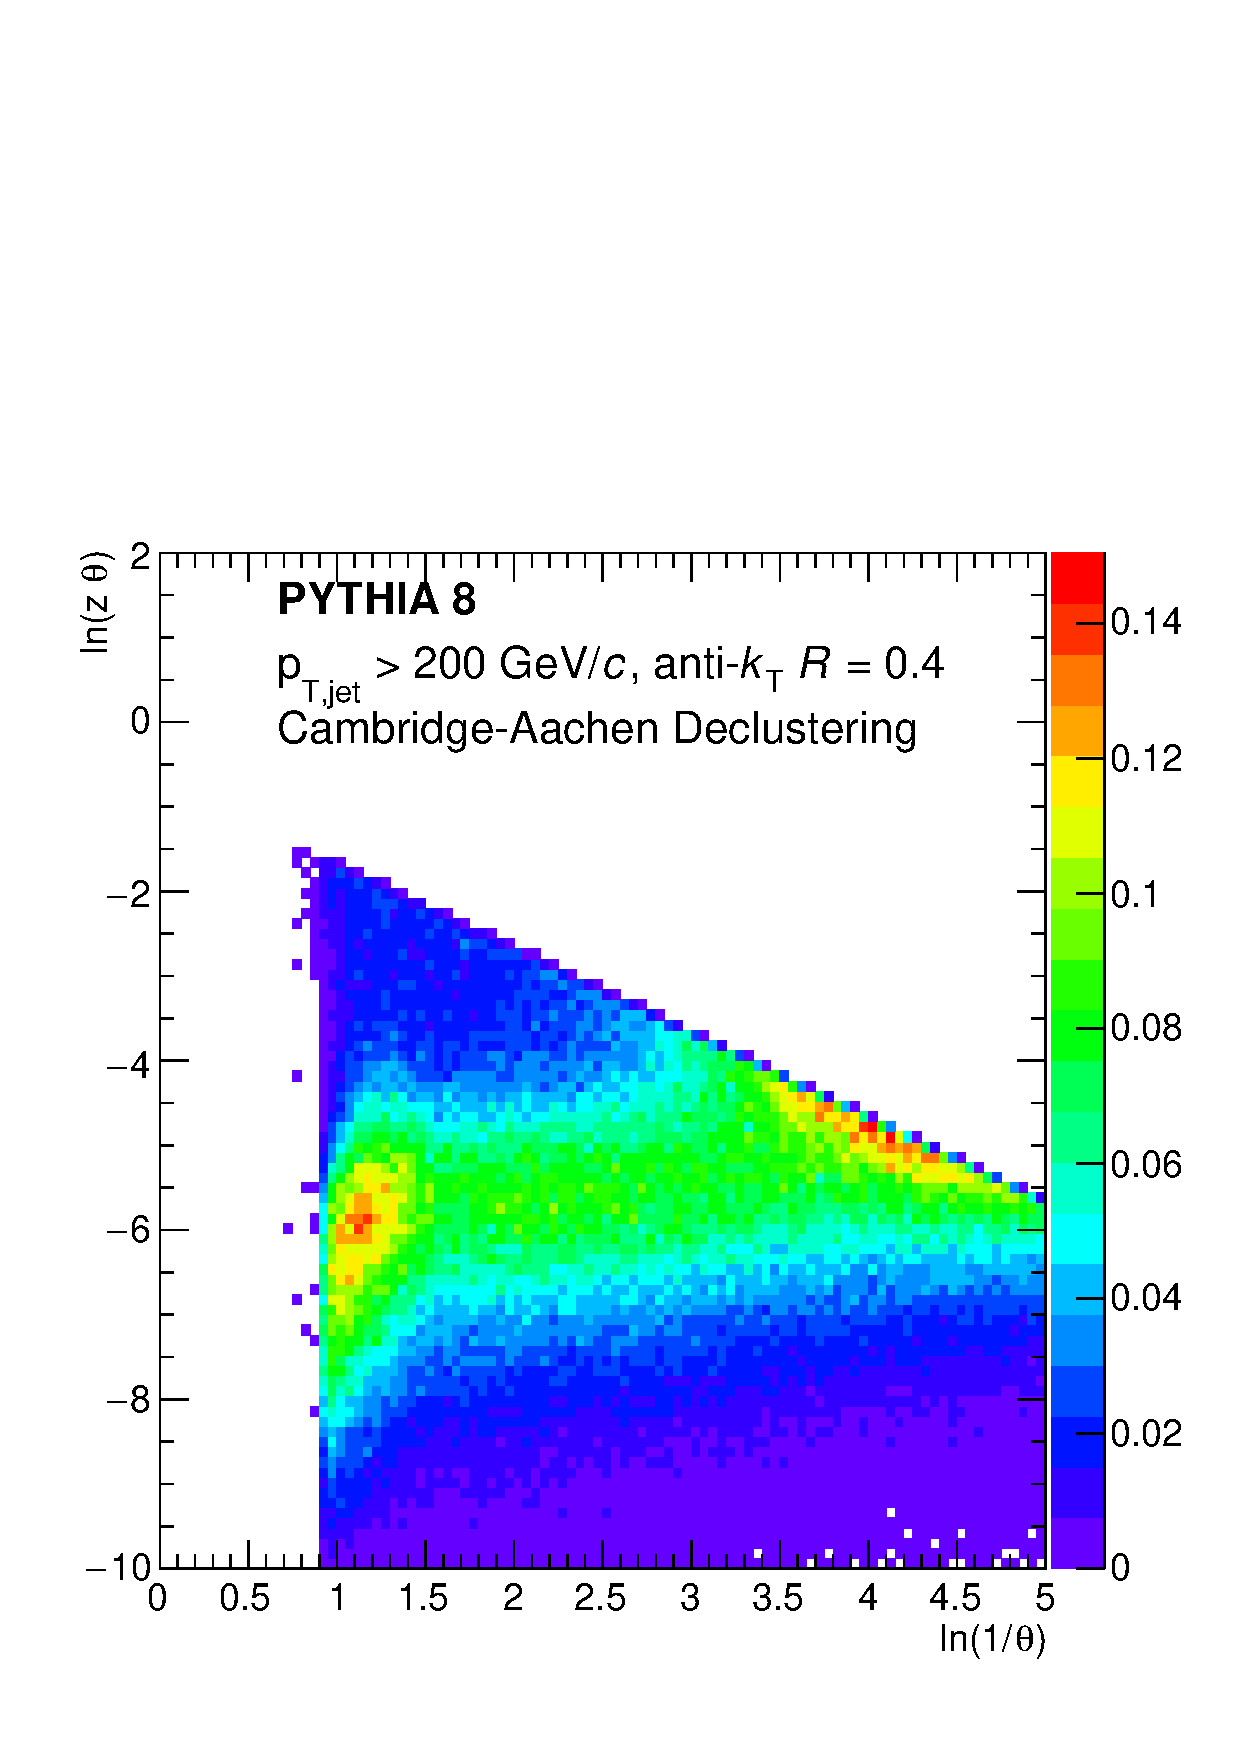
\includegraphics[width=0.33\textwidth]{figures/LundMC/Pythia_CA}
%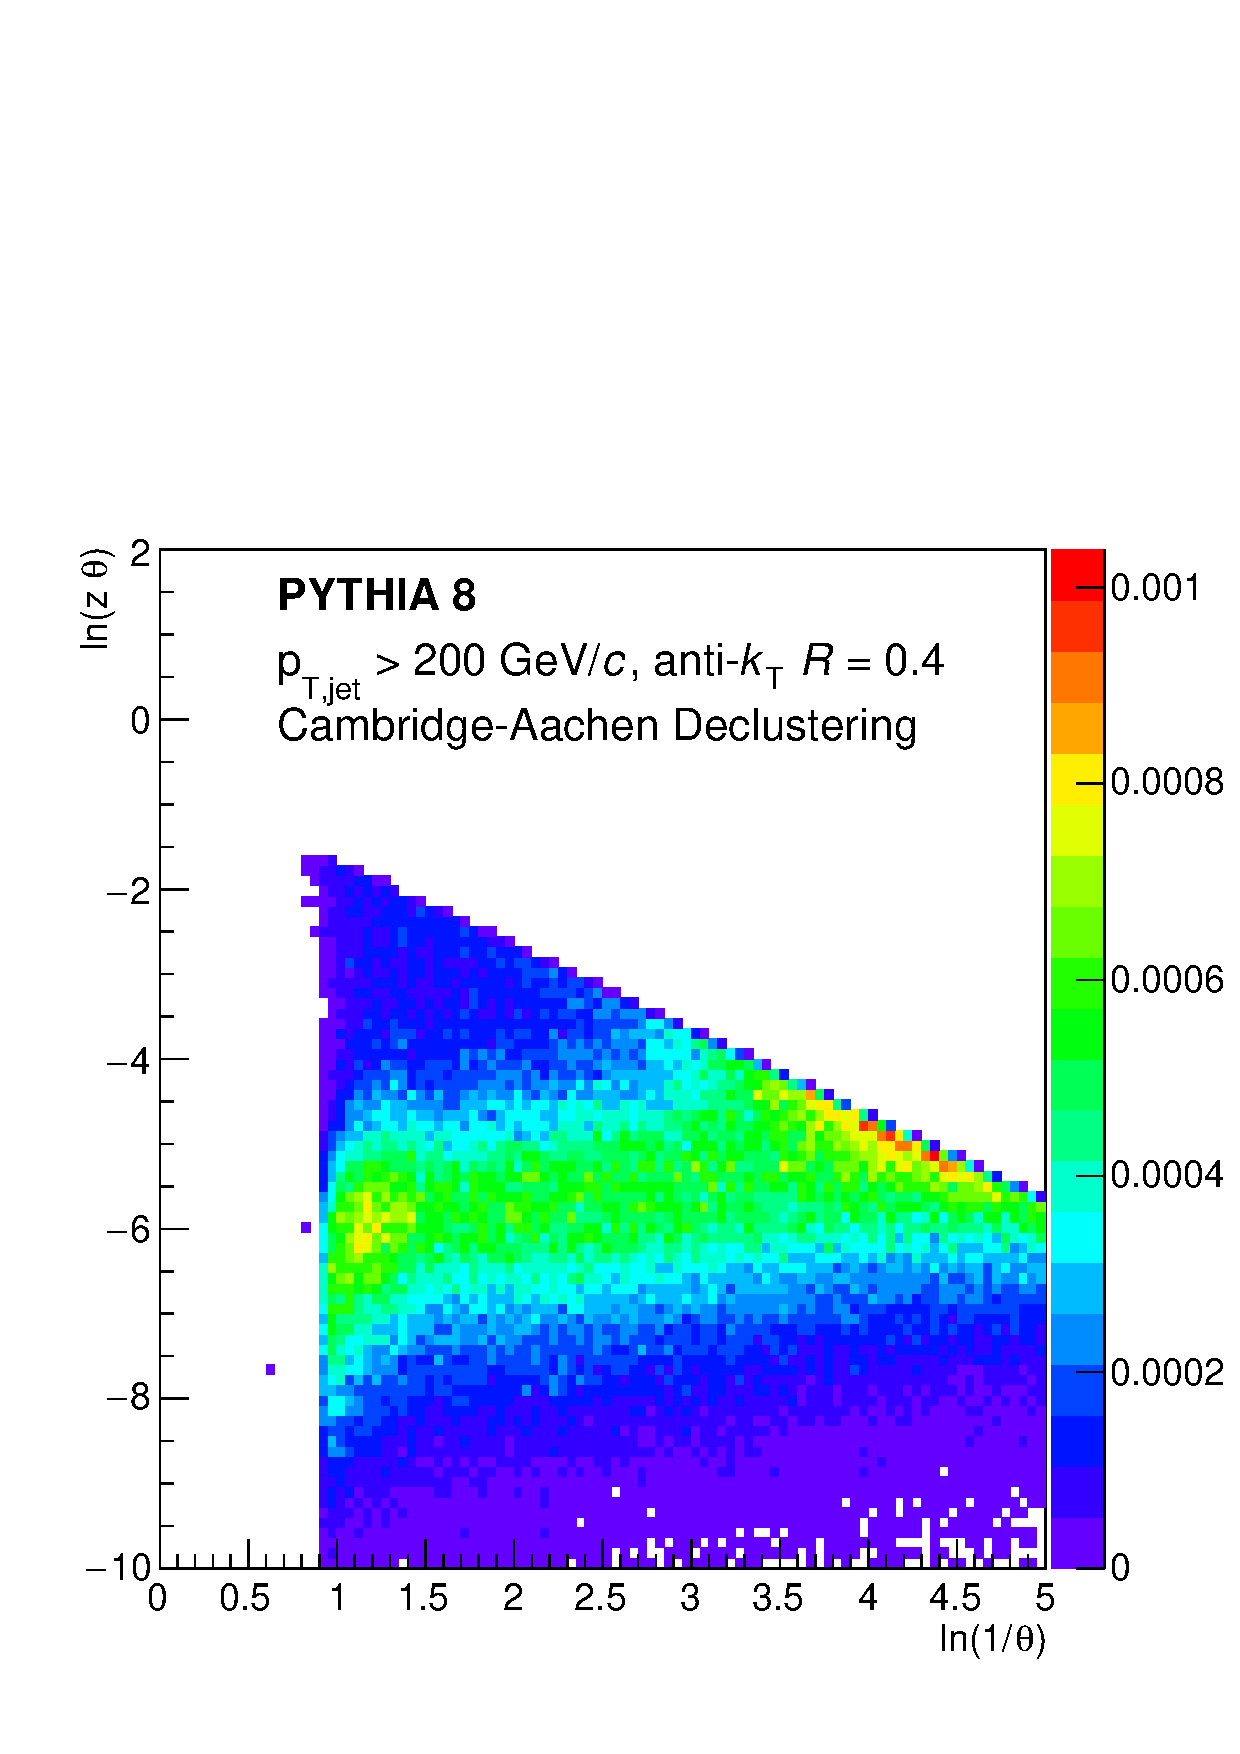
\includegraphics[width=0.4\textwidth]{figures/LundMC/Pythia_NoUE}
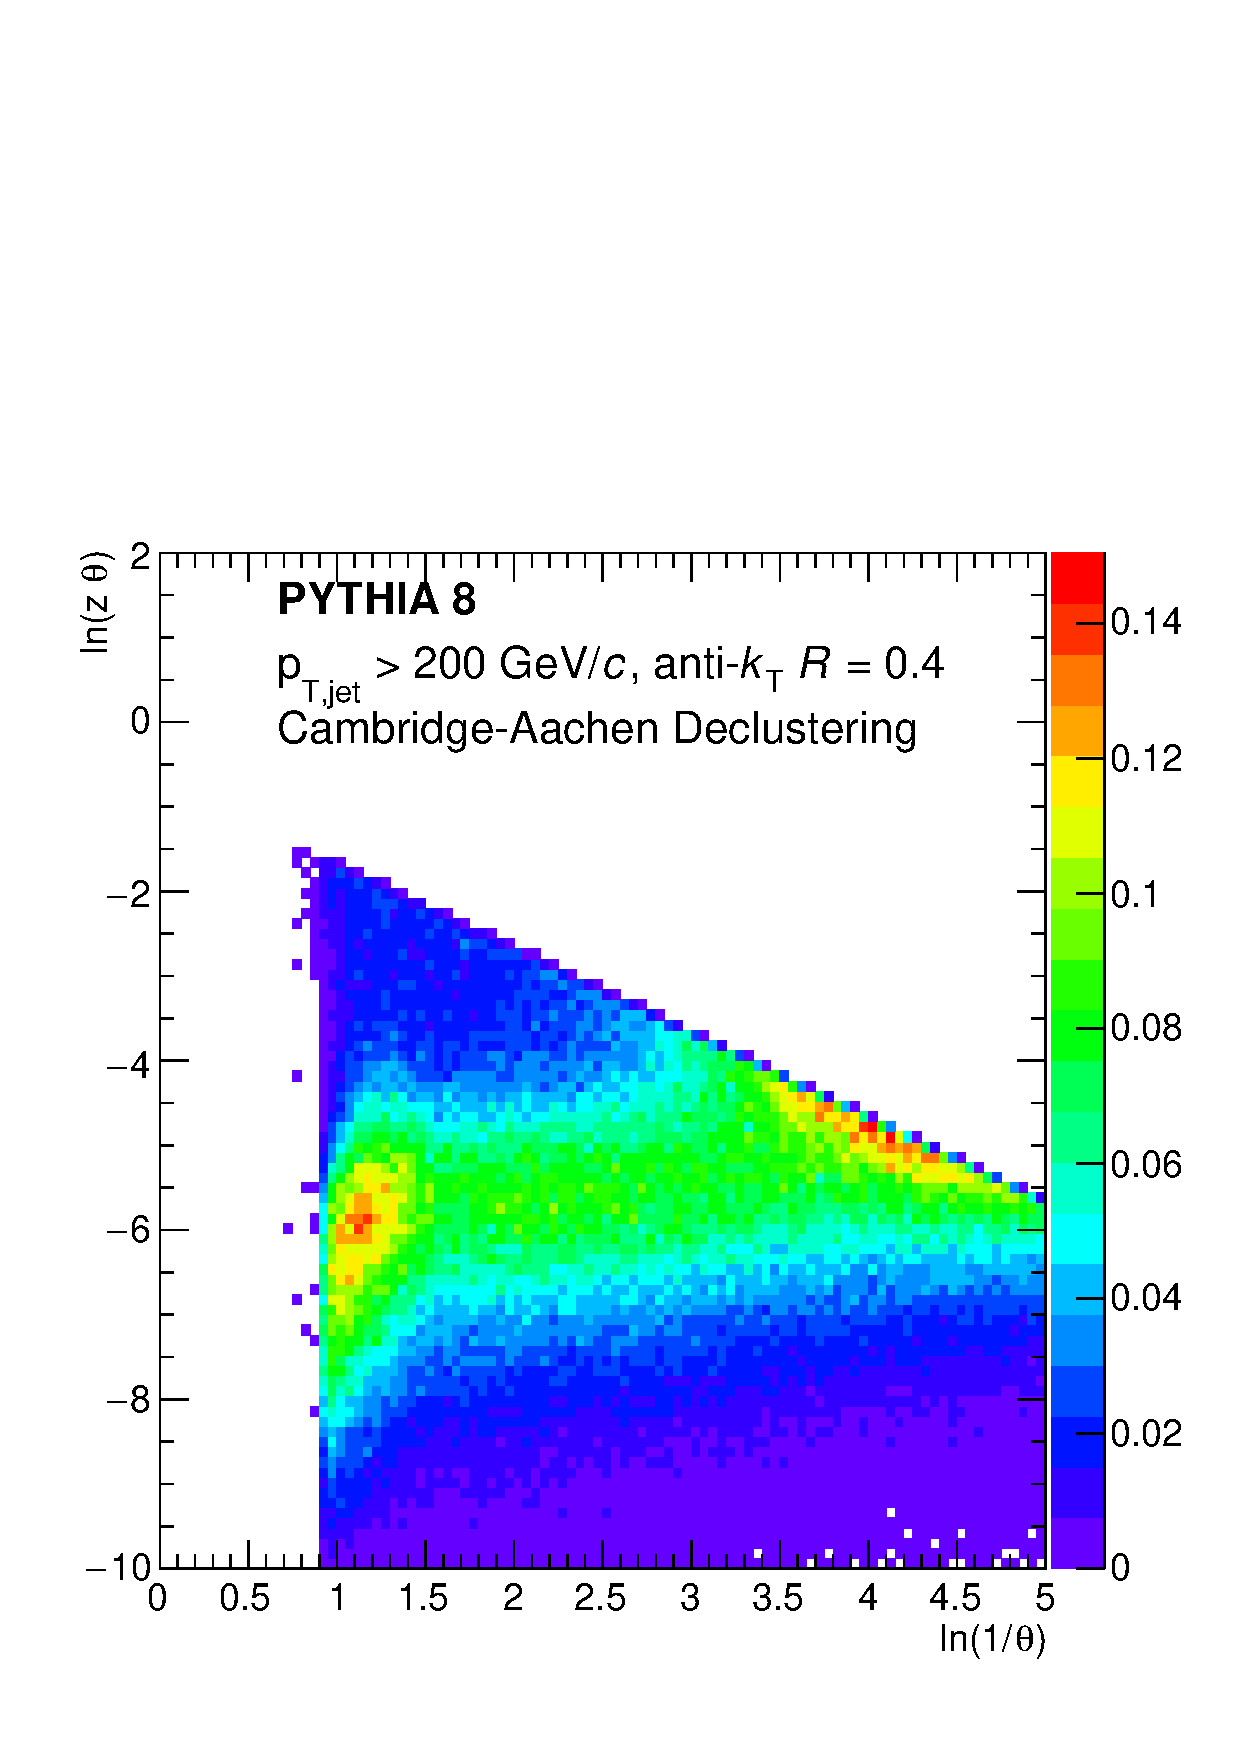
\includegraphics[width=0.33\textwidth]{figures/LundMC/Pythia_CA.pdf}%
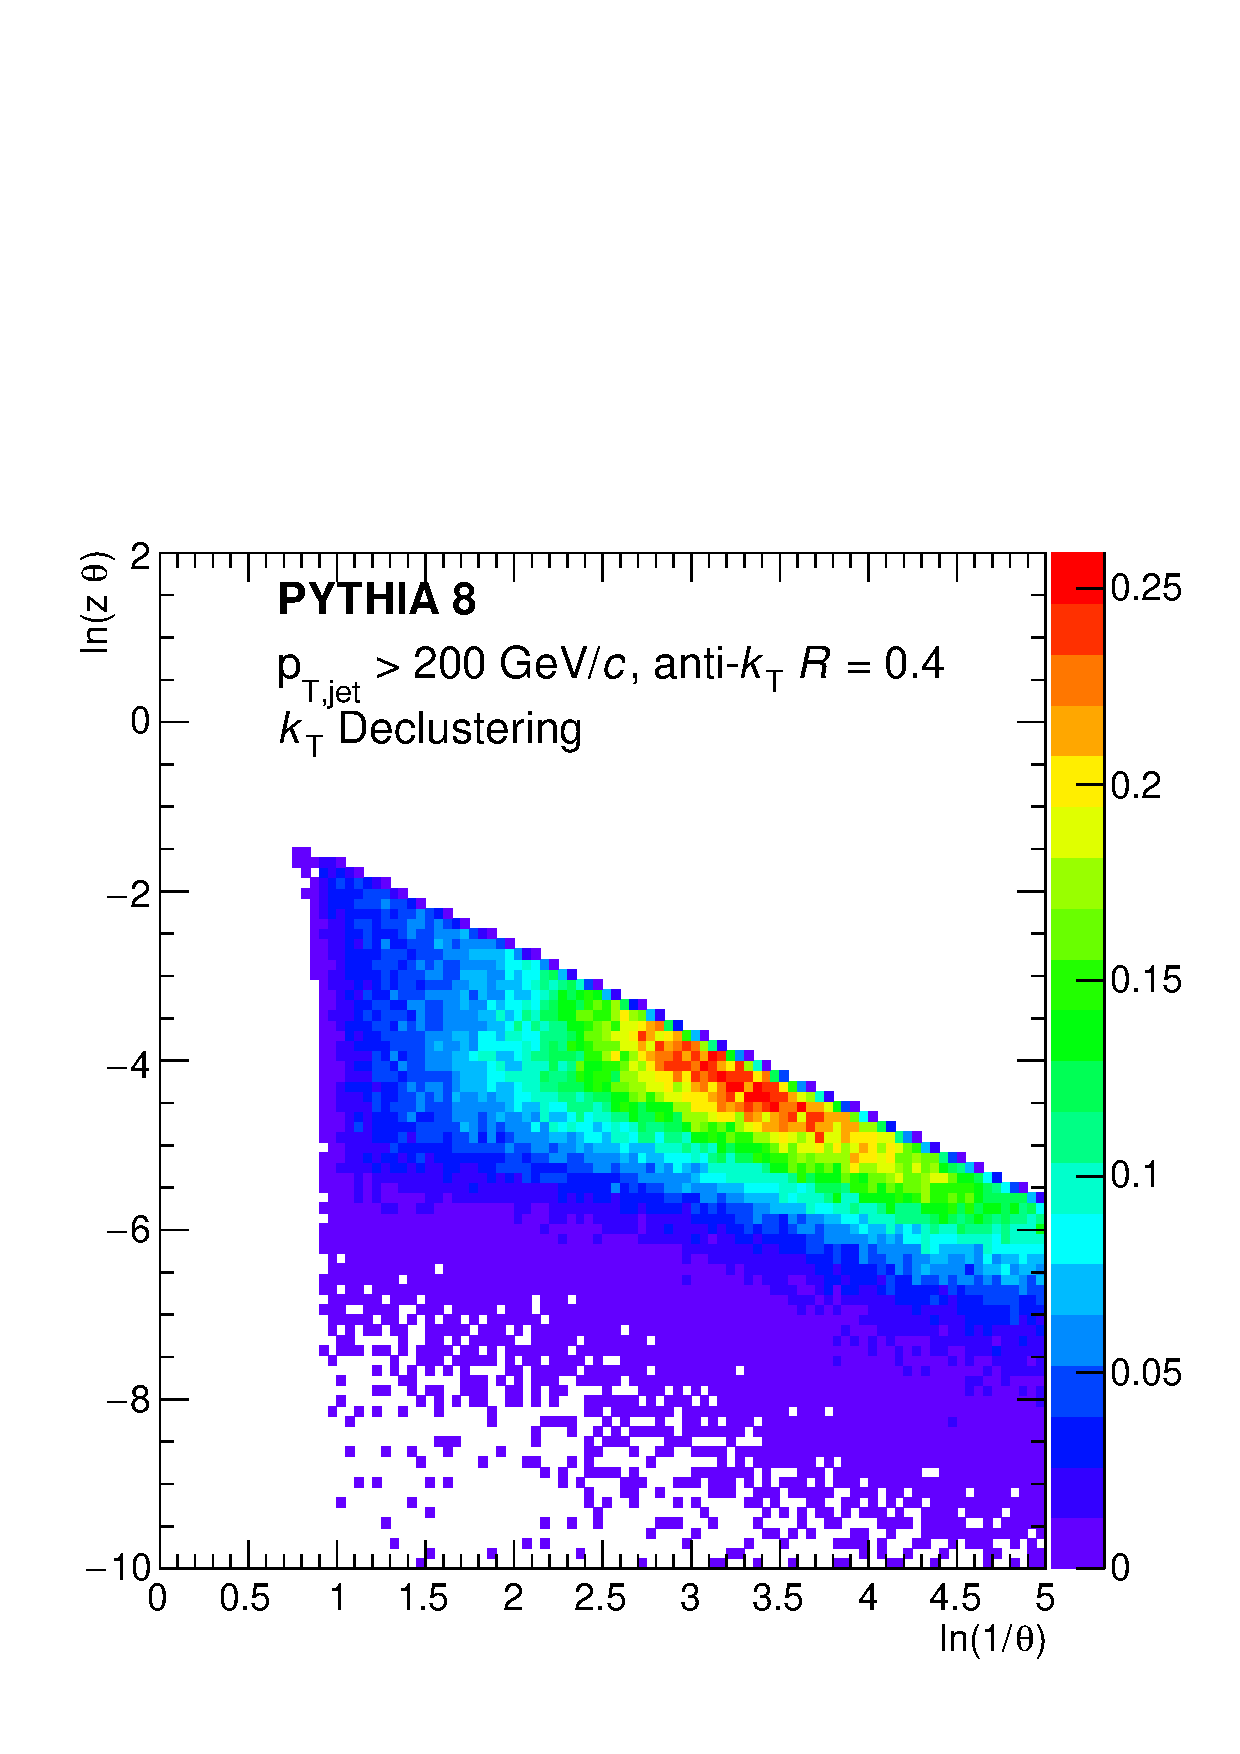
\includegraphics[width=0.33\textwidth]{figures/LundMC/Pythia_kt.pdf}%
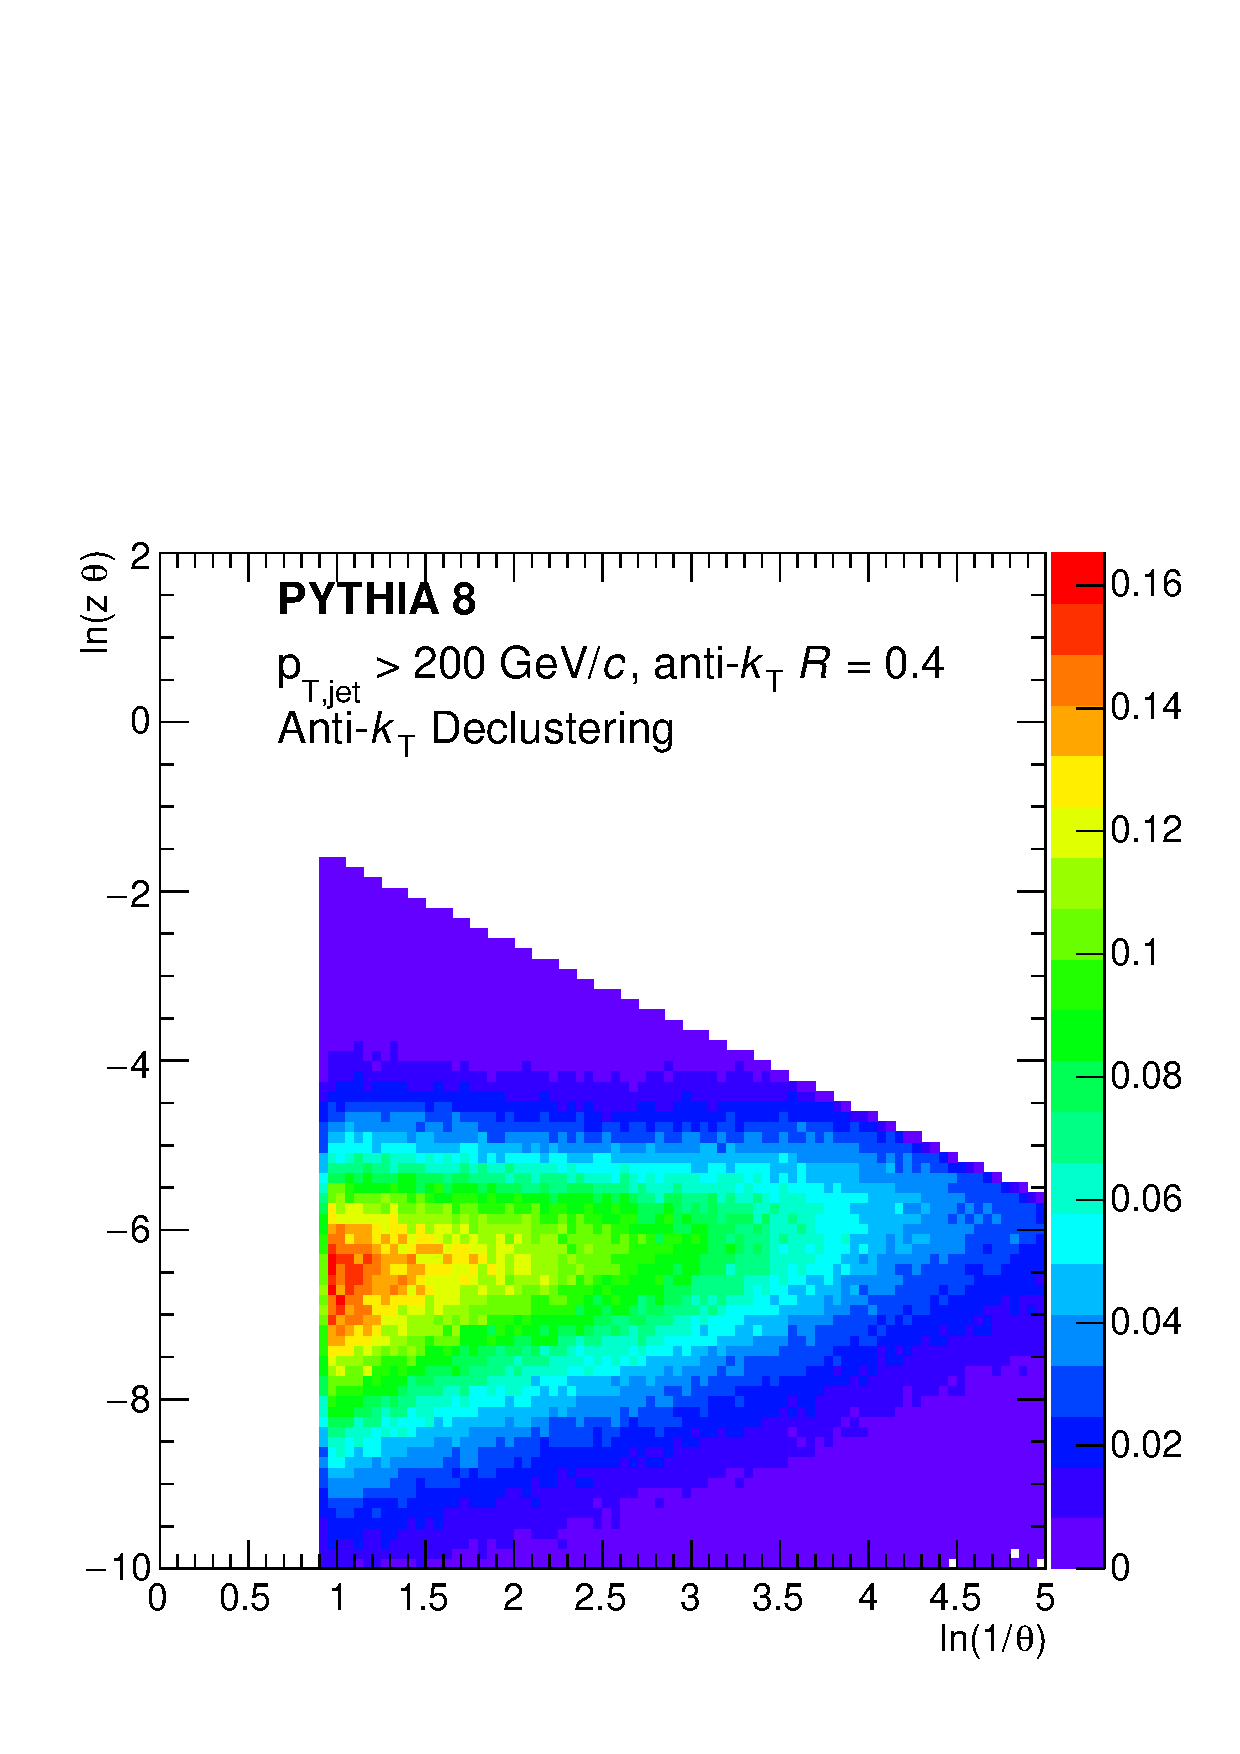
\includegraphics[width=0.33\textwidth]{figures/LundMC/Pythia_Akt.pdf}%
\caption{Lund diagrams reconstructed from a sample anti-$k_{\rm \tiny T} = 0.4$ jets generated by PYTHIA8. Three reclustering strategies were considered: C/A (left), $k_{\rm \tiny T}$(middle), and anti-$k_{\rm \tiny T}$ (right).}
\label{fig:PS2Vac}
\end{figure}
%%%%%%%%%%%%%%%%%%%%%%%%%%%%%%%%%%%%%
Using this procedure for the three different reclustering algorithms, we analyzed a sample of jet generated by PYTHIA in \autoref{fig:PS2Vac}. The jet sample corresponds to reconstructed anti-$k_{\rm \tiny T} = 0.4$ jets with $\pT > 200 $ GeV/c. The expected, simple features are nicely realized for the C/A reclustering, see \autoref{fig:PS2Vac} (left). In particular, we see a slow enhancement of radiation at fixed $k_\perp$ which can mainly be attributed to running-coupling effects. The additional features can be attributed to effects from the underlying event that was not subtracted in this sample. Indeed, the maps generated by the (anti-)$k_{\rm \tiny T}$ reclustering are not uniform and possess and enhanced sensitivity to collinear, \autoref{fig:PS2Vac} (center), and soft, large-angle configurations, \autoref{fig:PS2Vac} (right), as naively expected.

%%%%%%%%%%%%%%%%%%%%%%%%%%%%%%%%%%%%%
\begin{figure}[t!]
\centering
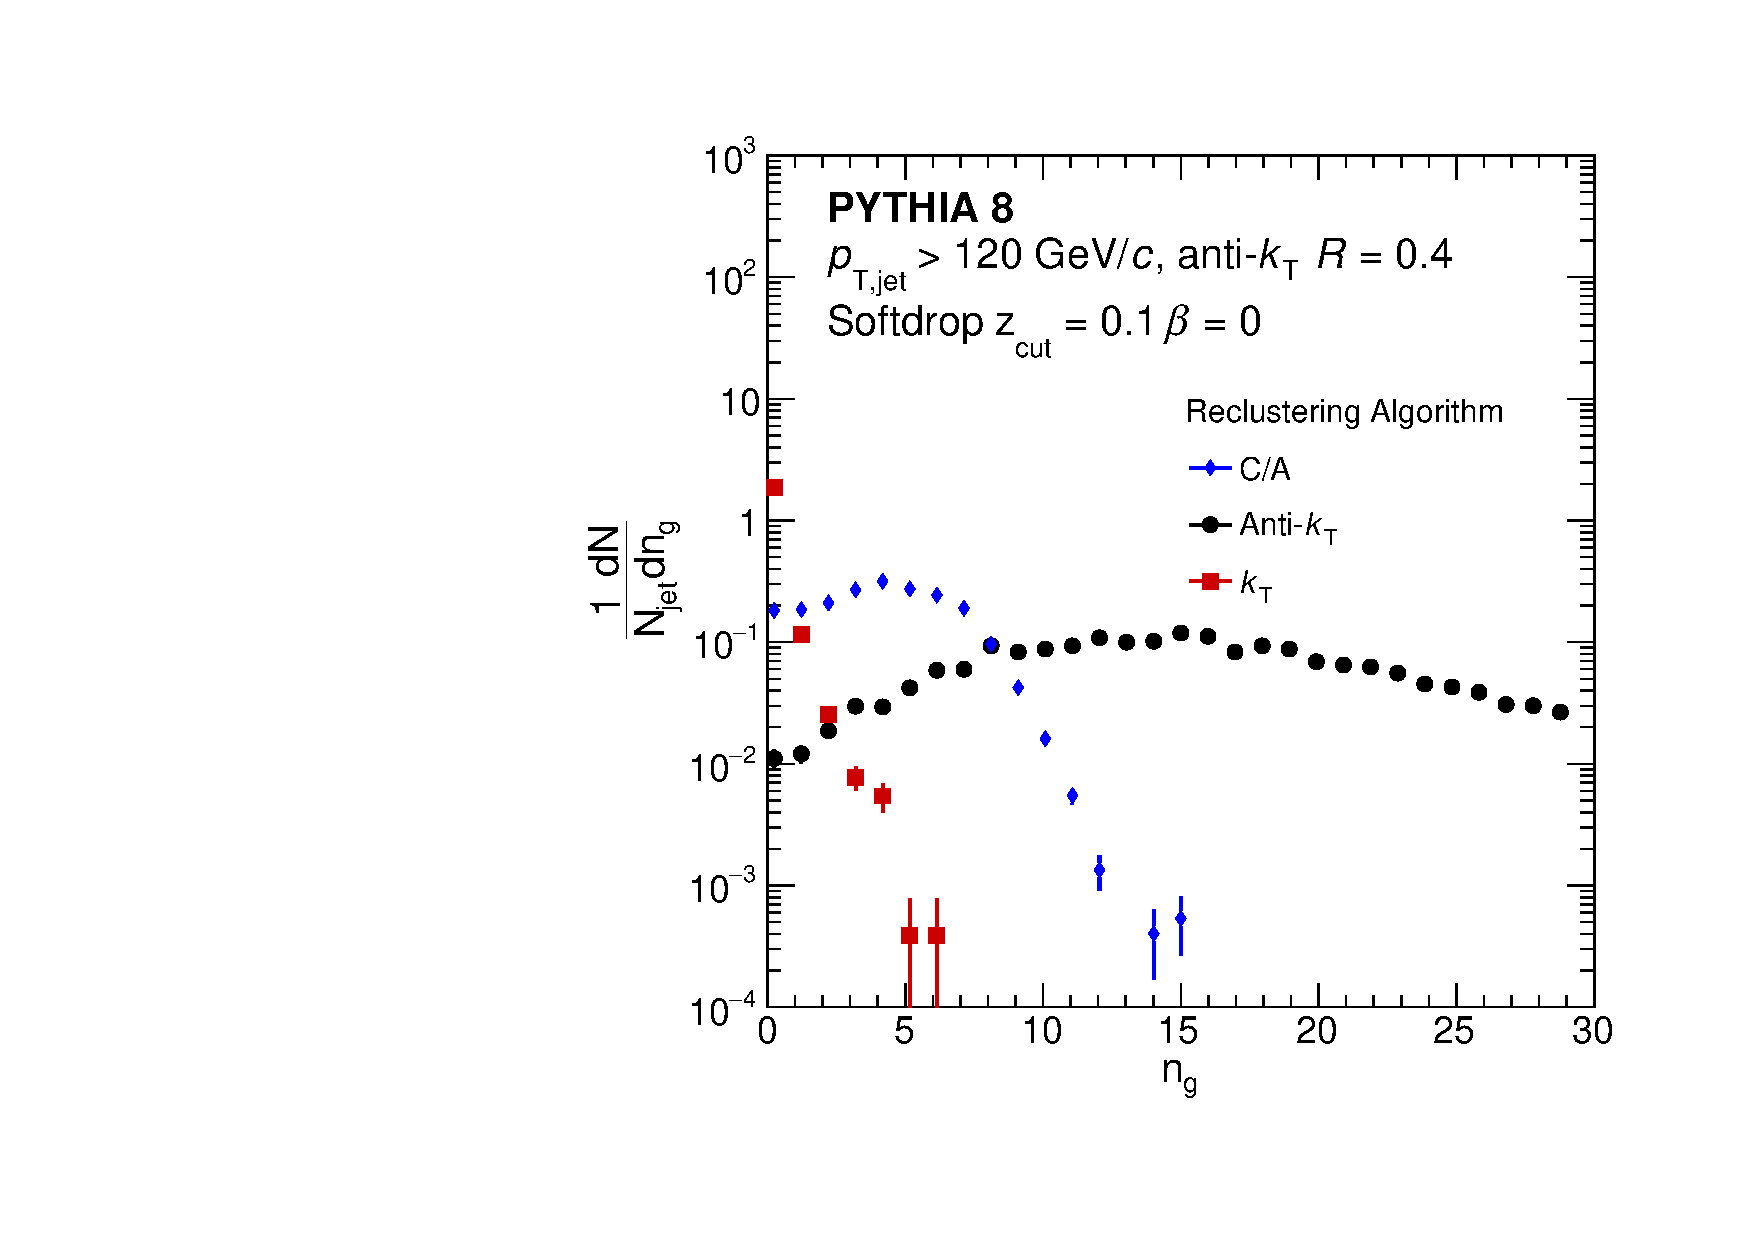
\includegraphics[width=0.4\textwidth]{figures/SDAlgorithms/ndropClusteringComp.pdf}%
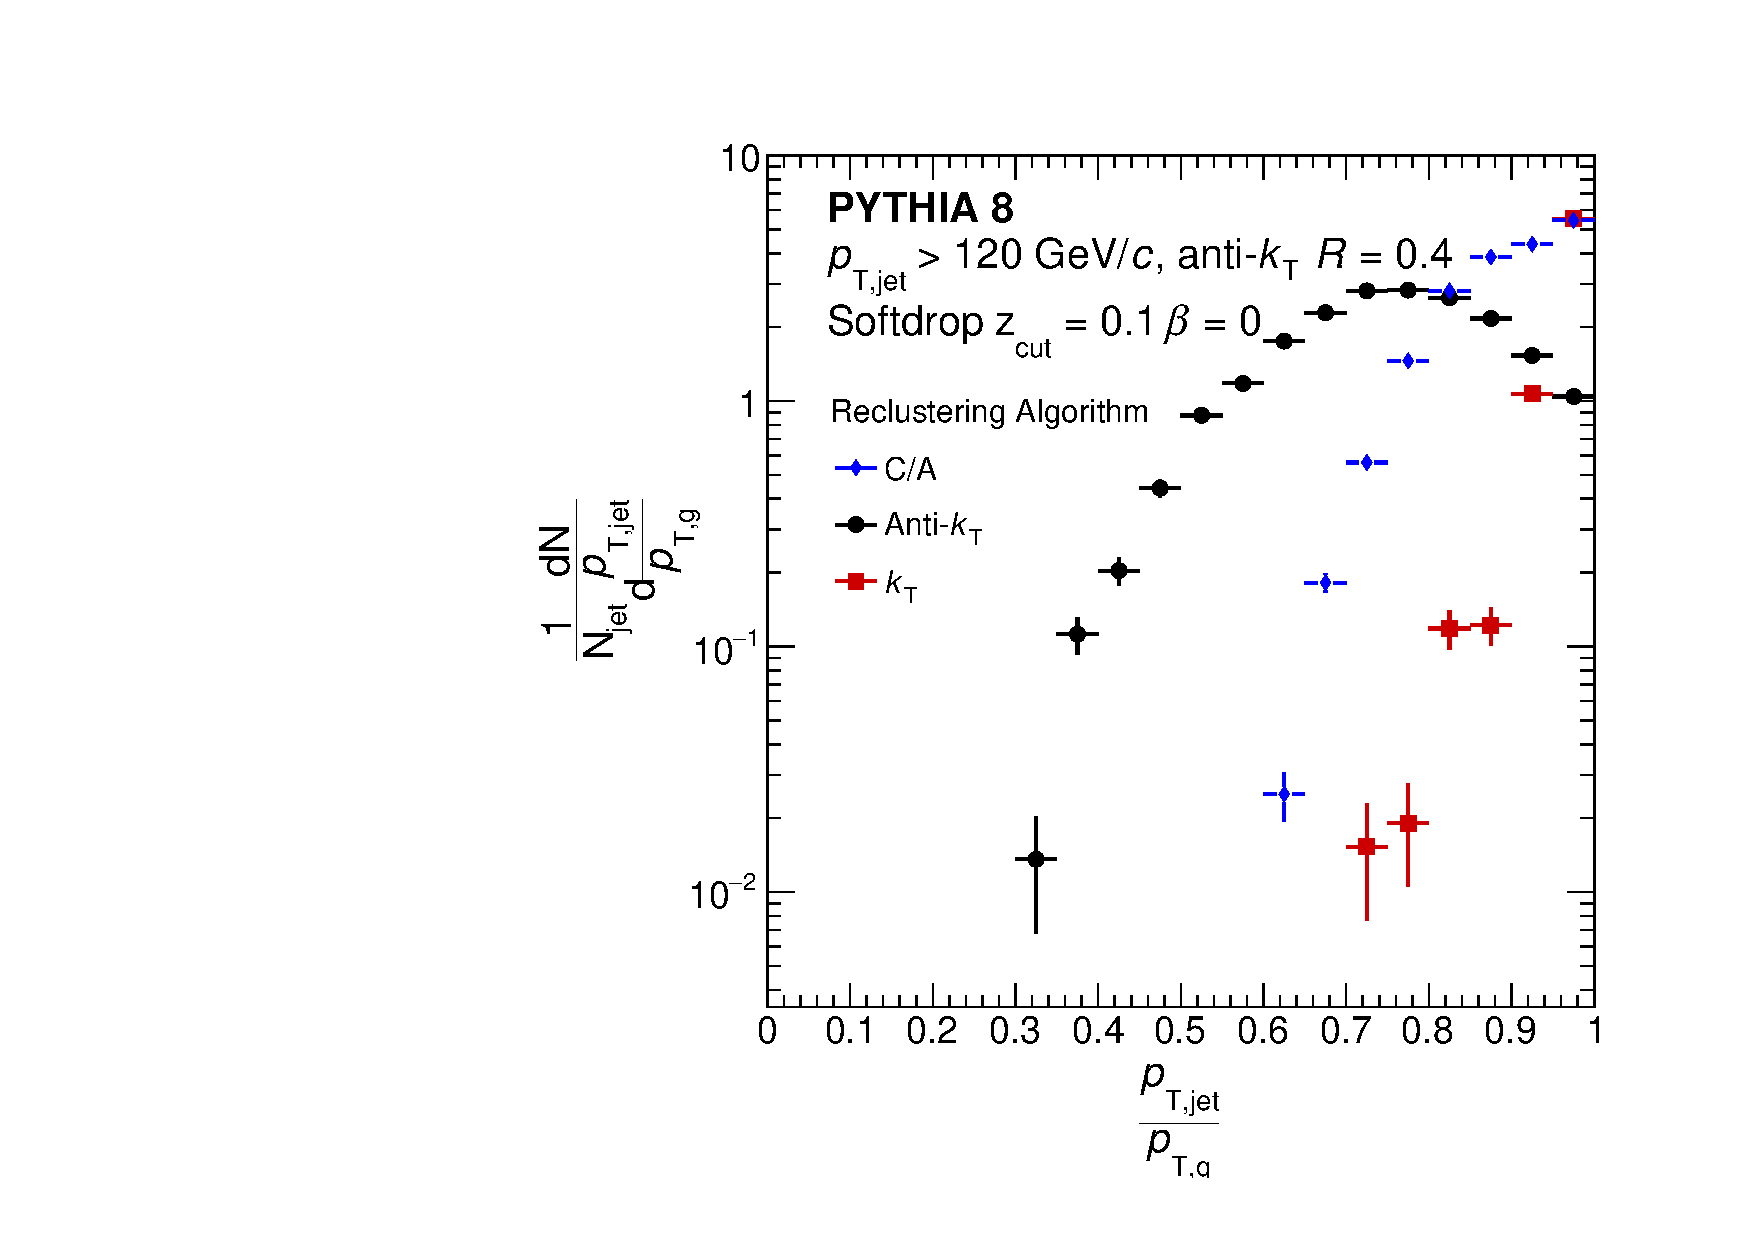
\includegraphics[width=0.4\textwidth]{figures/SDAlgorithms/ptratioClusteringComp.pdf}%
\caption{Effects of grooming on trees that are built up using different reclustering algorithms. Left plot: number of grooming steps. Right plot: ratio of jet $\pT$ before and after grooming.}
\label{fig:PS2Vac_2}
\end{figure}
%%%%%%%%%%%%%%%%%%%%%%%%%%%%%%%%%%%%%
The change of algorithm also strongly affects what happens to the jet after grooming. In \autoref{fig:PS2Vac_2} (left), we show the distribution of the number of grooming steps for the three reconstruction algorithms discussed above. In particular, we note that the $k_\perp$ and the anti-$k_\perp$ algorithms result in completely different grooming. While the jet reconstructed with the former algorithm are mainly unaffected by grooming, in the latter case of the order of $\sim 10-20$ branches are groomed away. This also strongly affects the $\pT$ of the groomed jet, as seen in \autoref{fig:PS2Vac_2} (right), where the groomed jets in the anti-$k_\perp$ sample on average lose $\sim 20$\% of their energy. The C/A algorithm falls in between the two extremes, as usual. Of the order of $\sim 5$ branches are removed by the grooming procedure on average, which slightly reduces the jet $\pT$ by $\lesssim 10$\%.

As pointed out before, medium-induced radiation does not per se follow the same (angular) ordering as described above. In fact, the resummation of soft radiation leads to quite different characteristics. We will however continue to apply the procedure outlined above to identify regions of particular medium modification in the following Section. Varying the reclustering algorithm can potentially enhance the sensitivity to different regimes, as found in the study above.


%{\color{red} Connect to discussion in the following sections.}

%%%%%%%%%%%%%%%%%%%%%%%%%%%%%%%%%%%%%%%%%
\subsection{Radiation phase space and sensitivity to jet quenching}
\label{sec:phasespace-mc}
%%%%%%%%%%%%%%%%%%%%%%%%%%%%%%%%%%%%%%%%%


%%%%%%%%%%%%%%%%%%%%%%%%%%%%%%%%%%%%%
\begin{figure}[h]
\centering
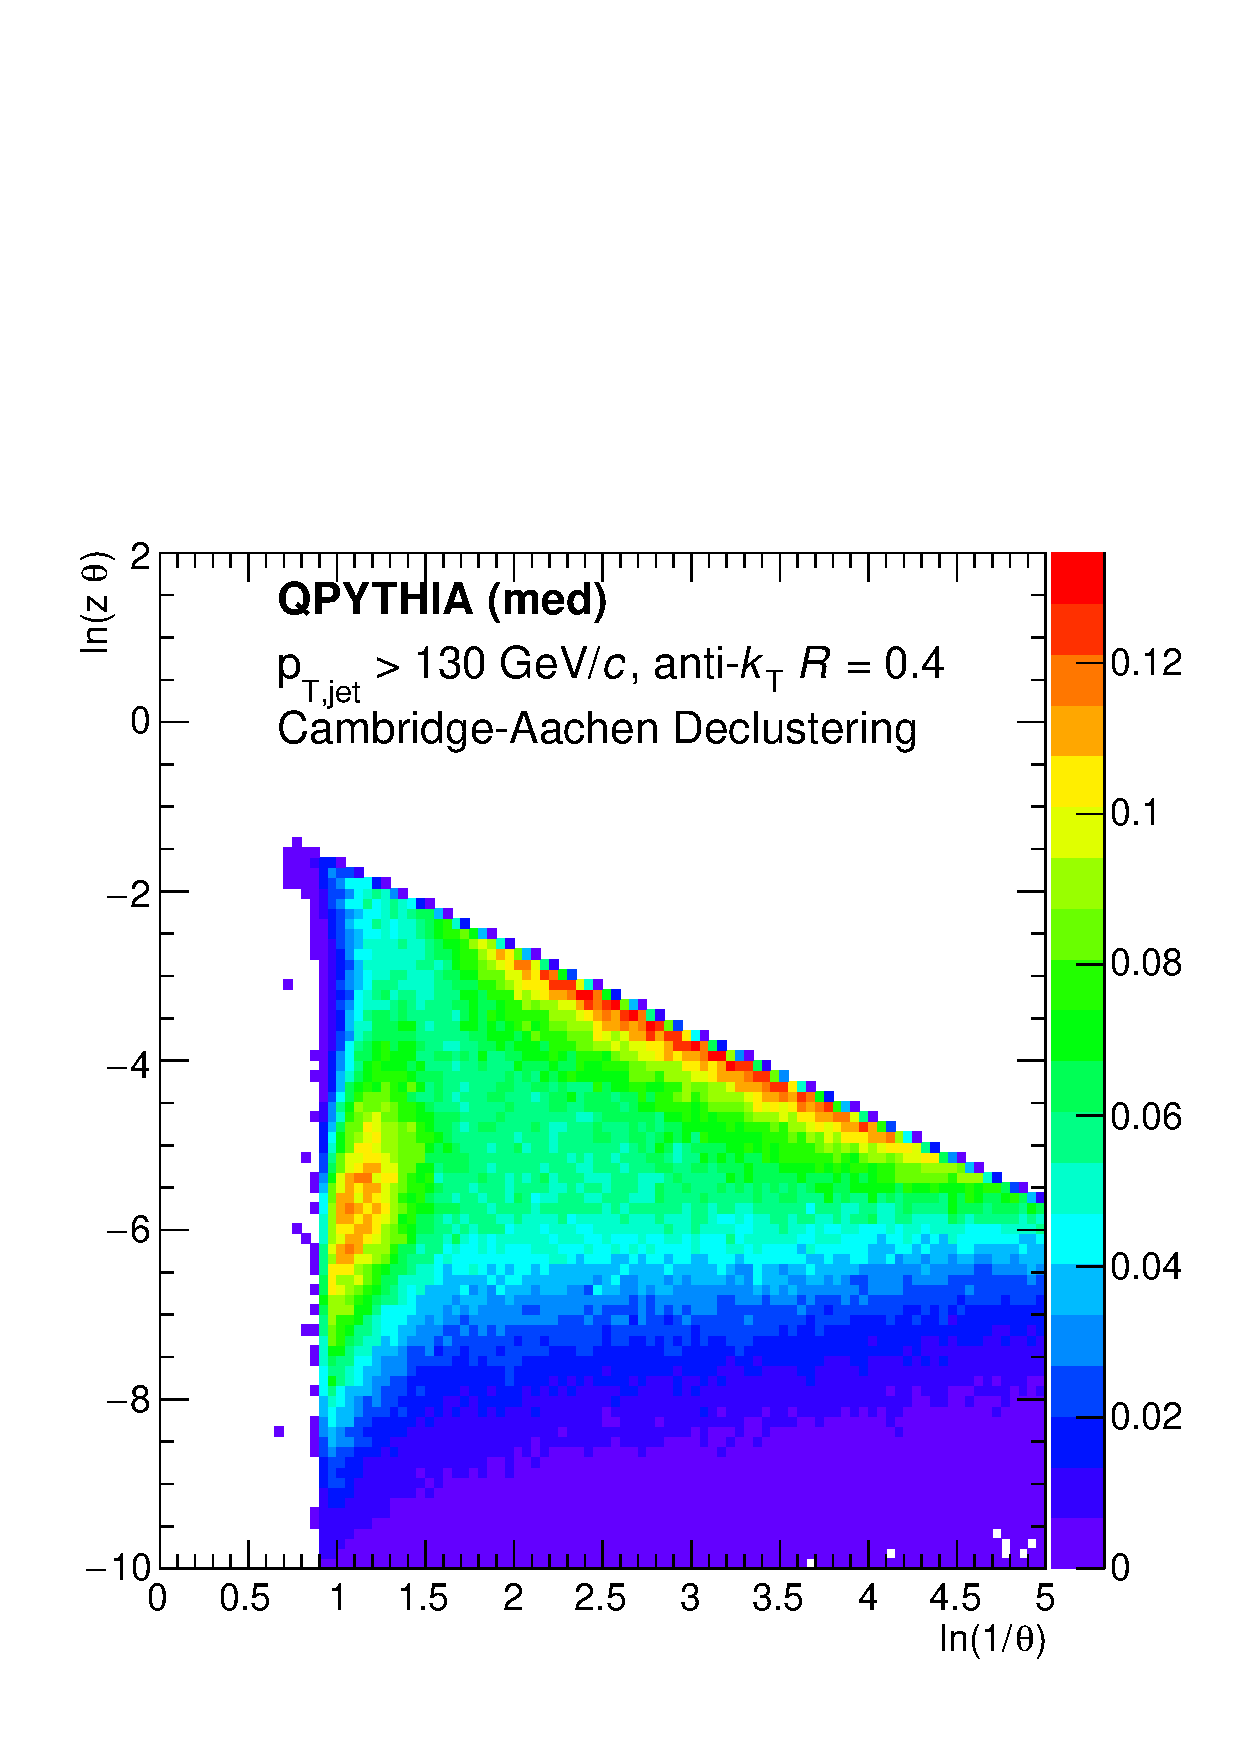
\includegraphics[width=0.3\textwidth]{figures/LundMC/QPythia_Med2}
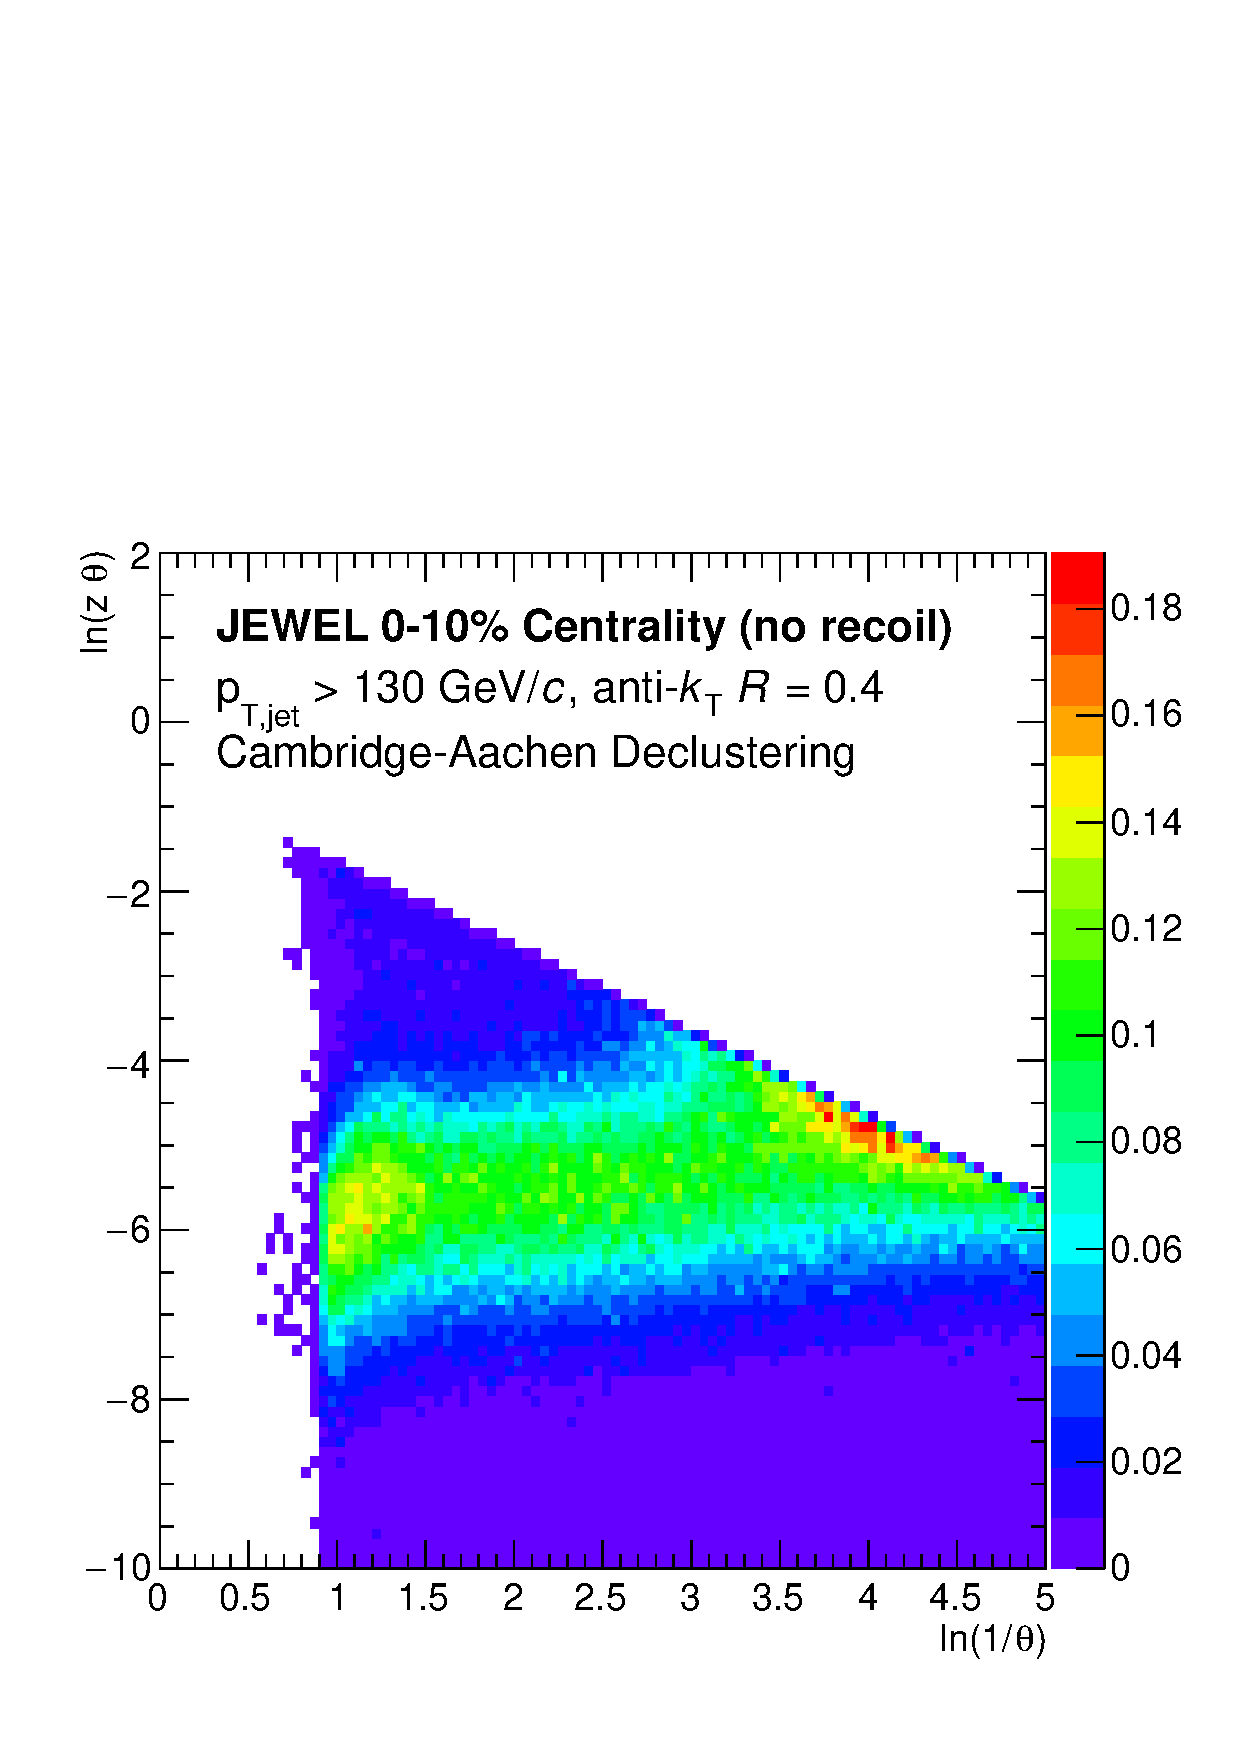
\includegraphics[width=0.3\textwidth]{figures/LundMC/Jewel_Med}
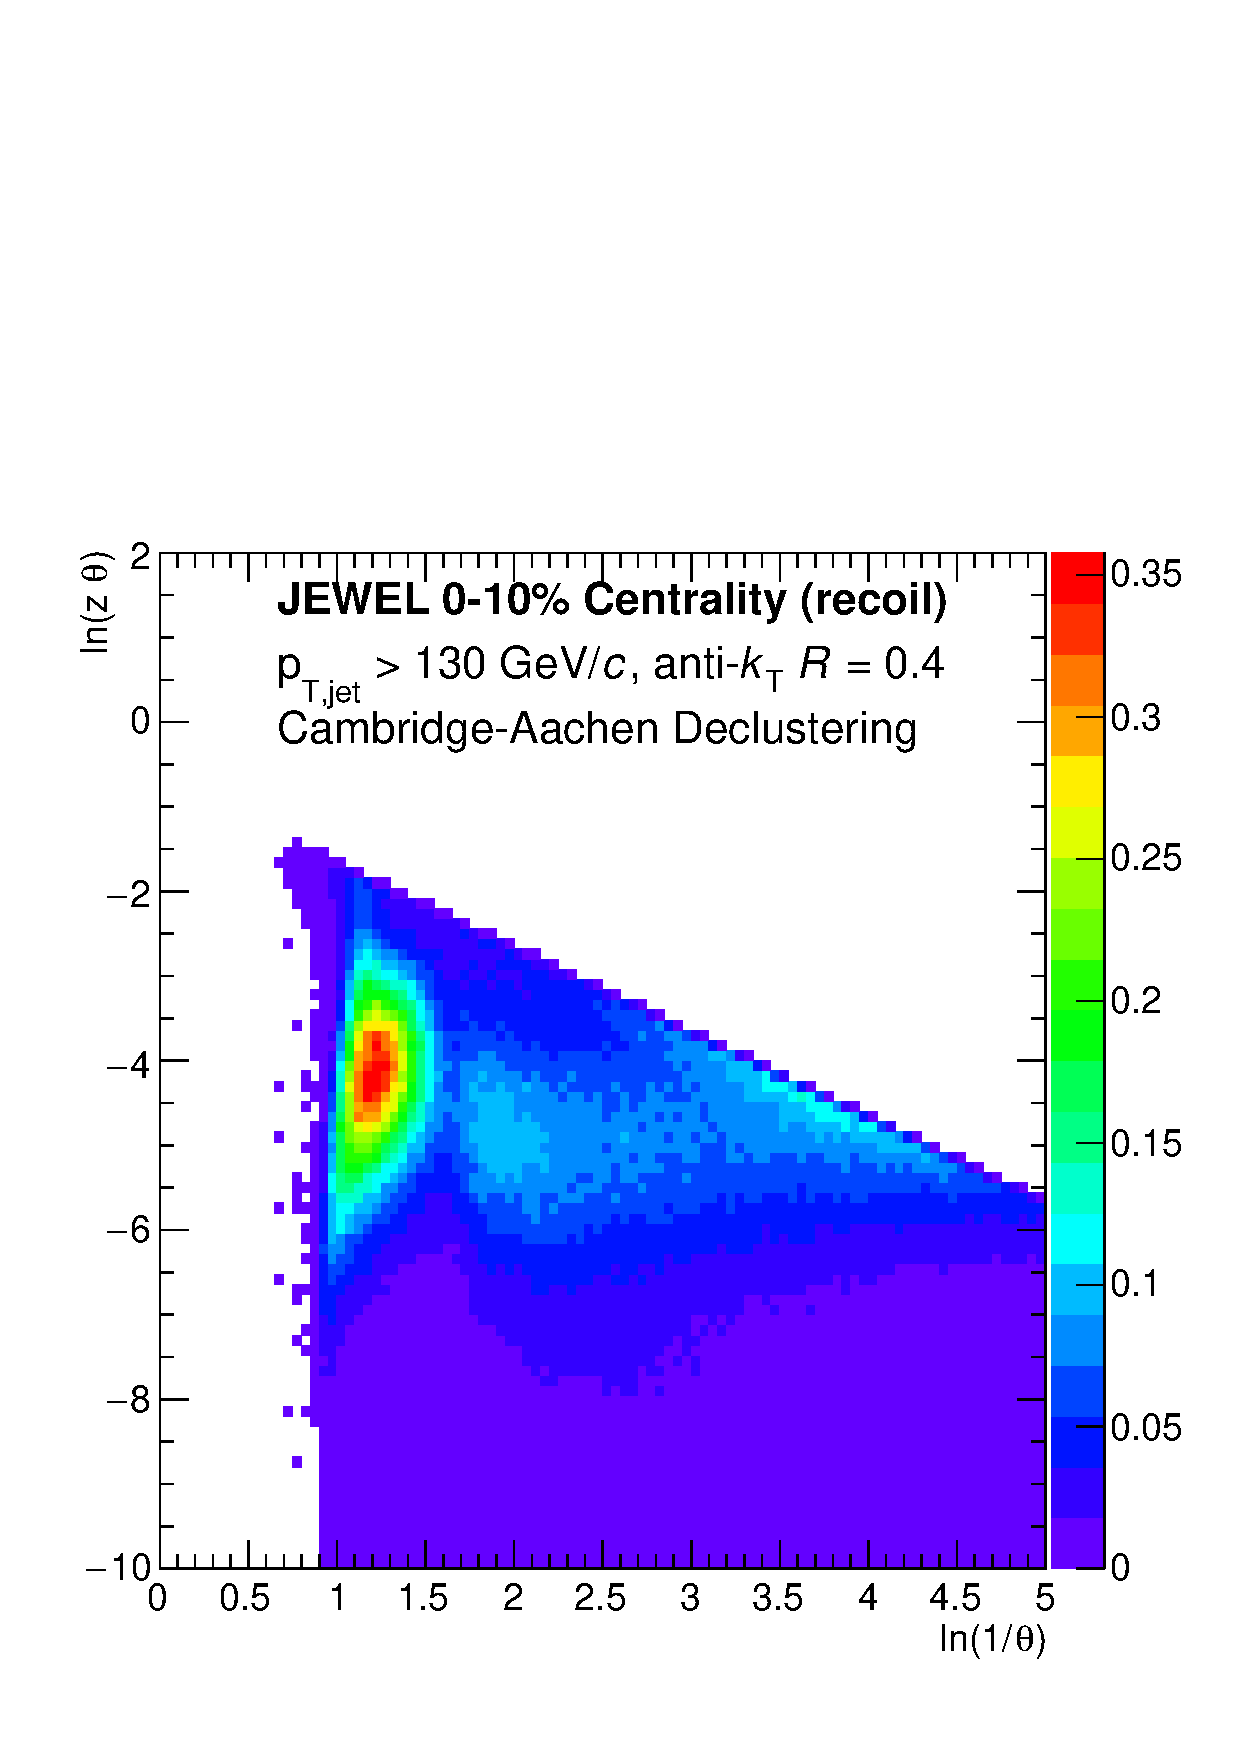
\includegraphics[width=0.3\textwidth]{figures/LundMC/Jewel_MedRecoil}
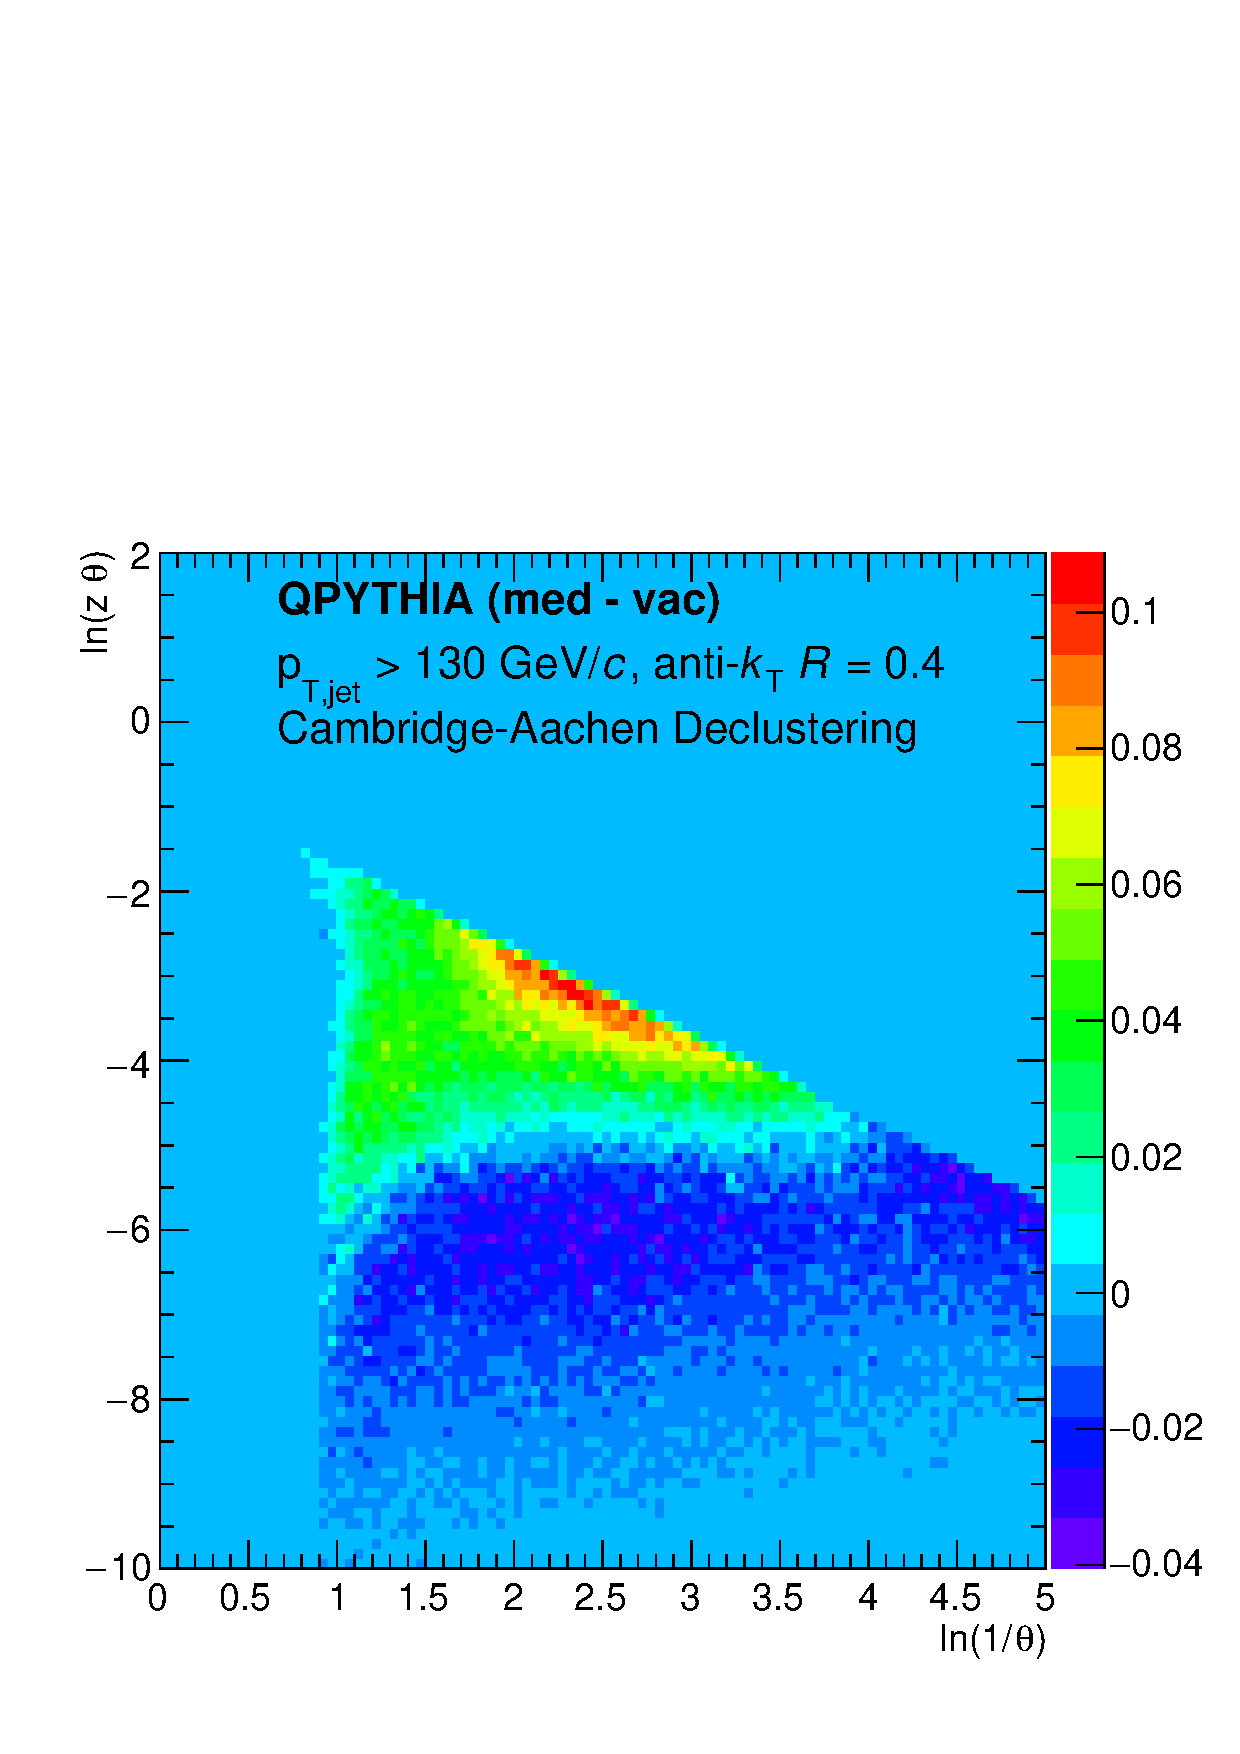
\includegraphics[width=0.3\textwidth]{figures/LundMC/QPythia_Diff}
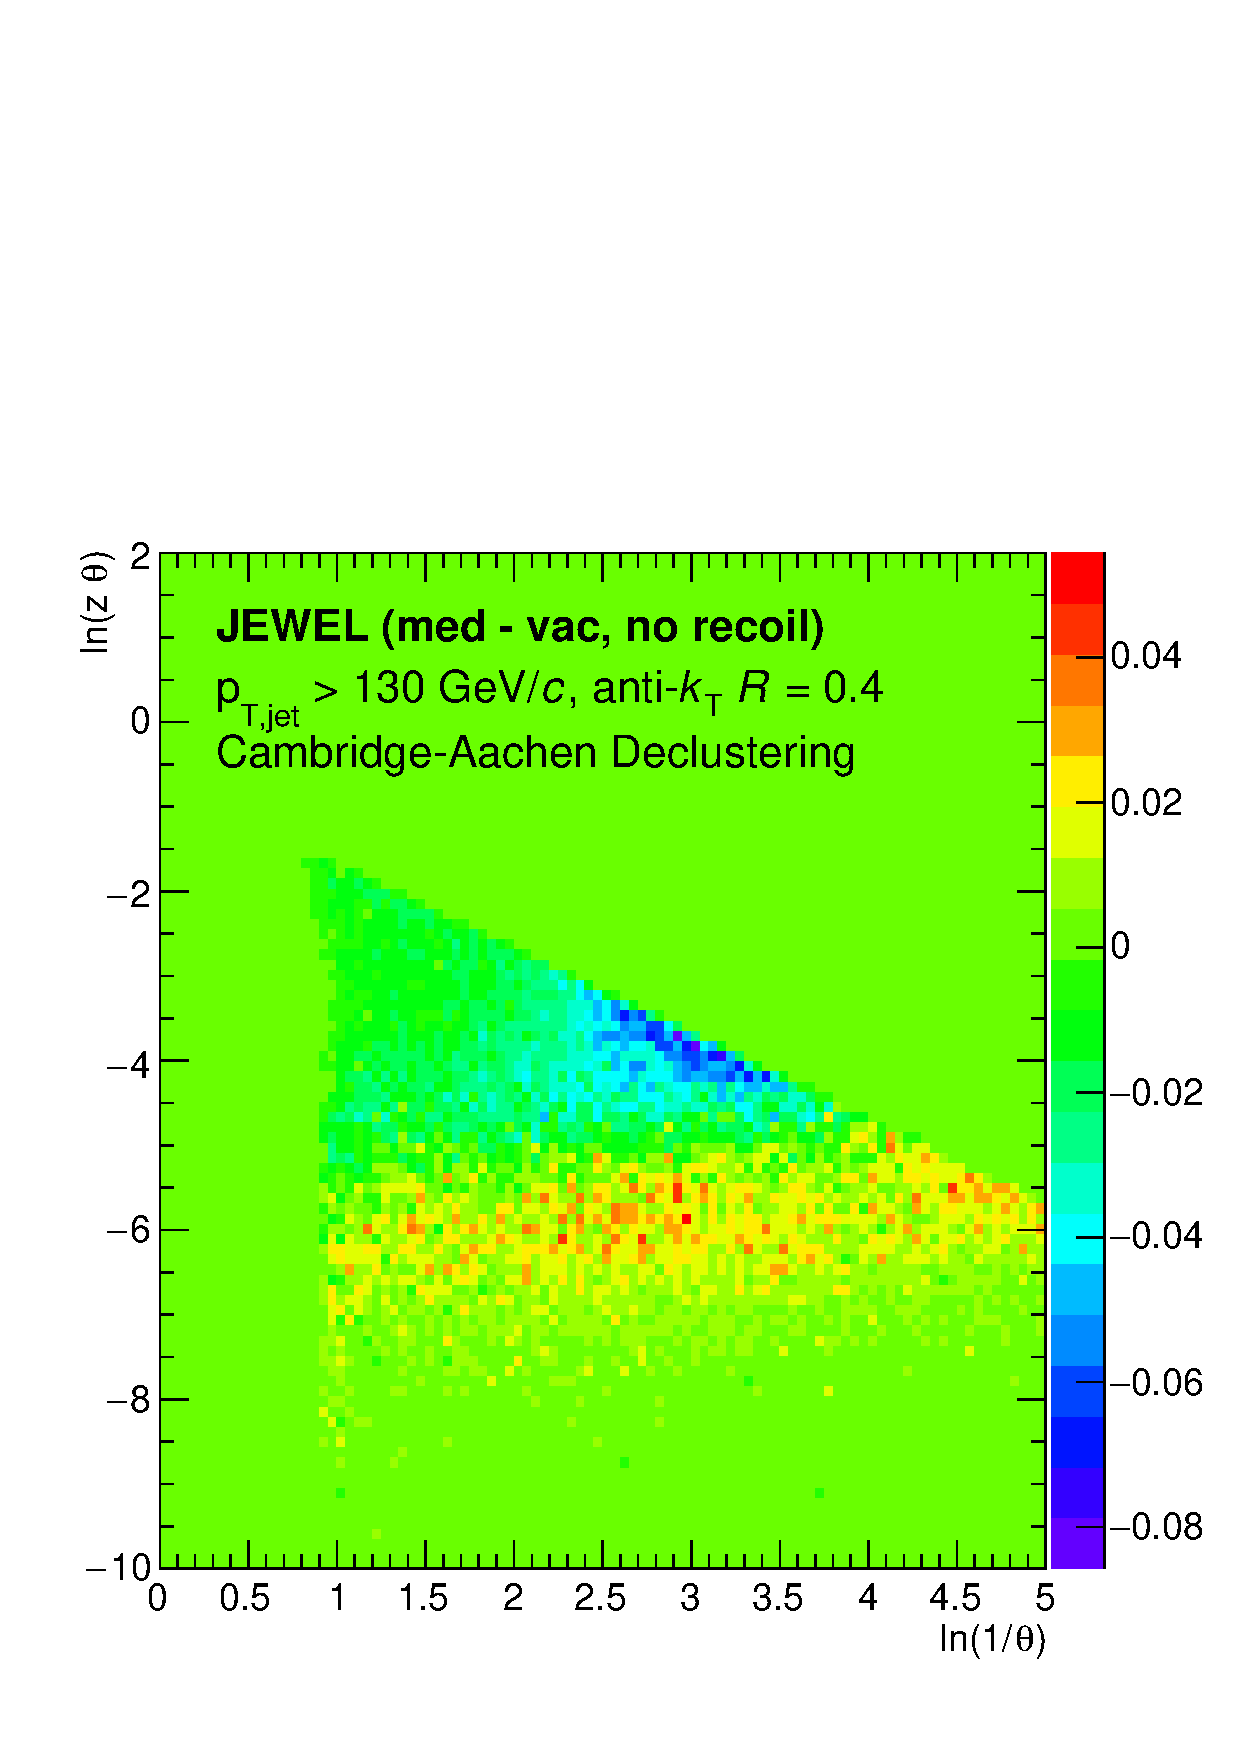
\includegraphics[width=0.3\textwidth]{figures/LundMC/Jewel_Diff}
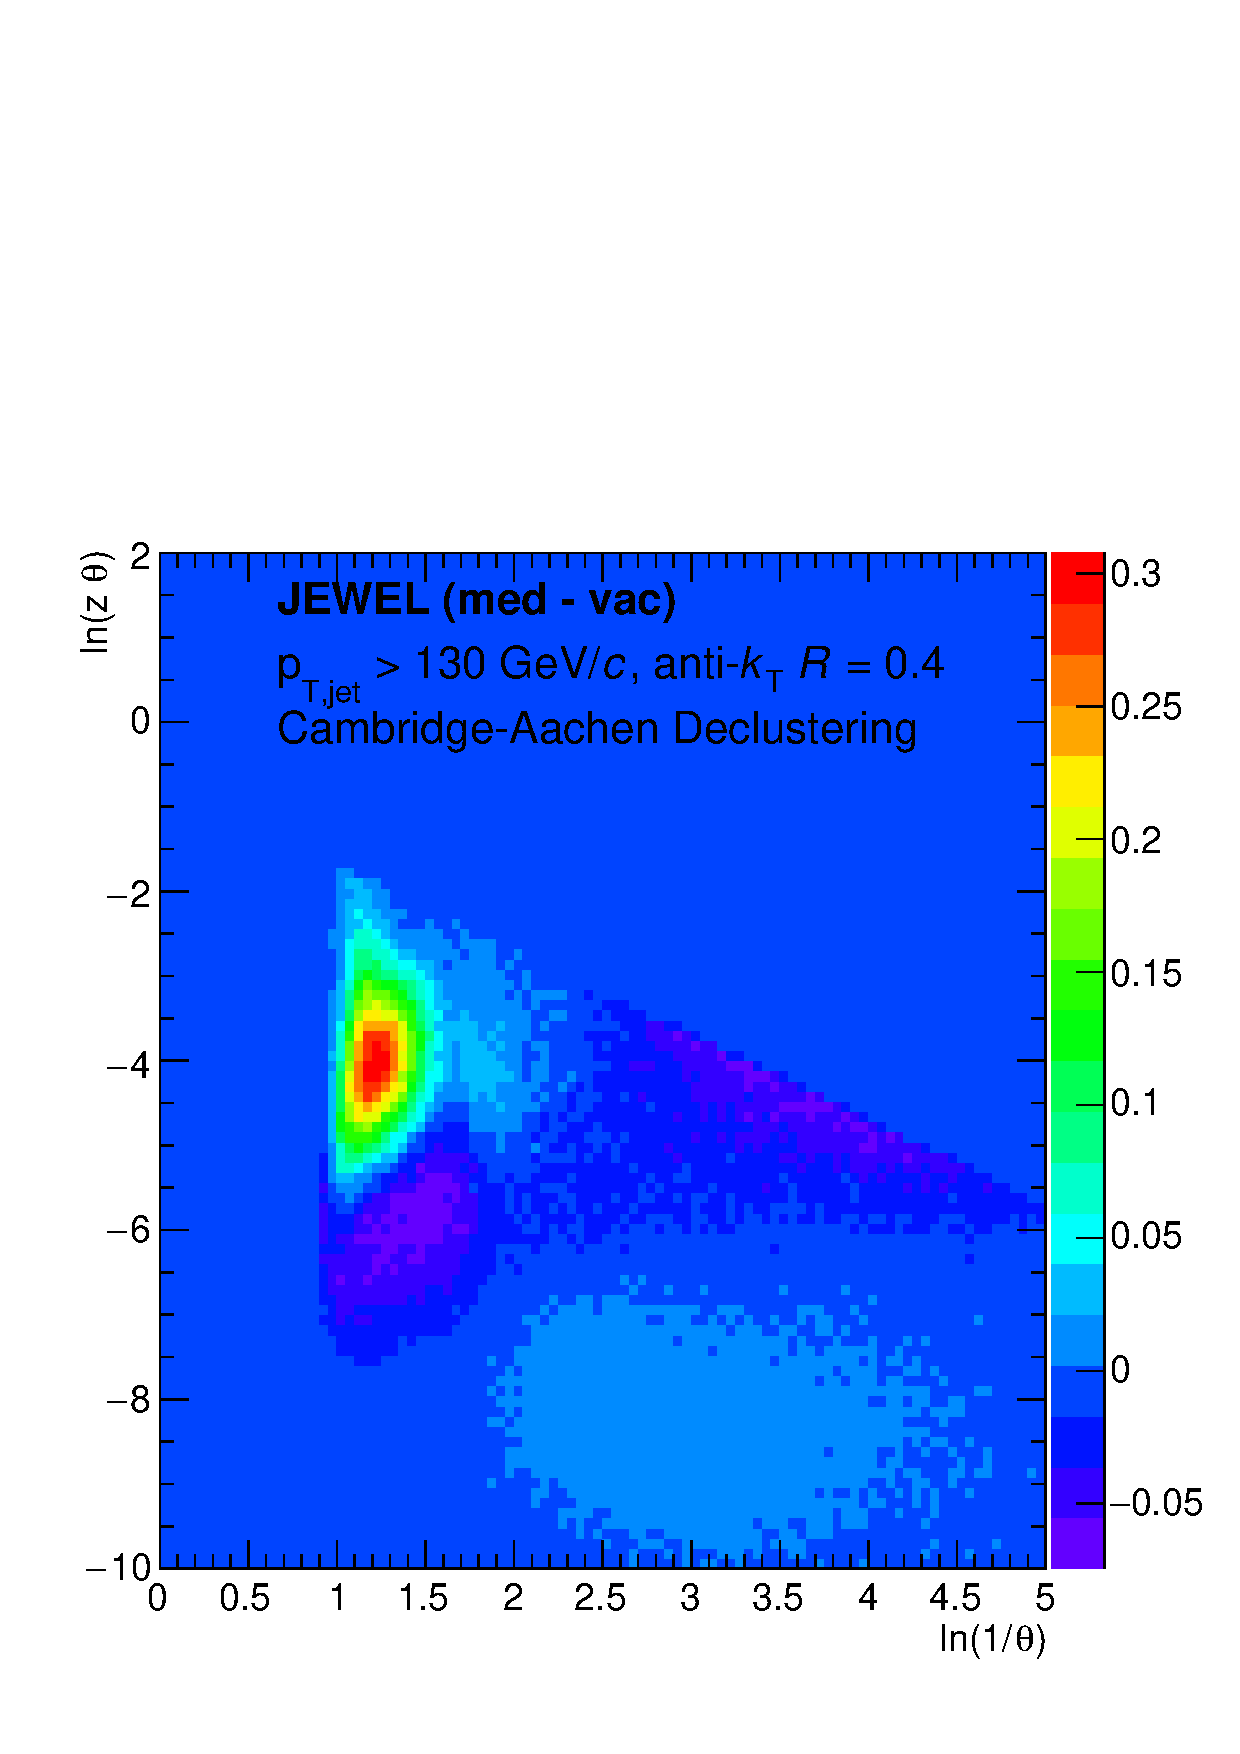
\includegraphics[width=0.3\textwidth]{figures/LundMC/Jewel_DiffRecoil}
\caption{Lund diagram reconstructed from jets generated by QPYTHIA (left column), JEWEL without recoils (middle column) and JEWEL with recoils (right column).
The lower panels correspond to the difference of the radiation pattern with and without jet quenching effects. Note that the scale of the $z$-axes varies between the panels.}
\label{fig:PS2}
\end{figure}
%%%%%%%%%%%%%%%%%%%%%%%%%%%%%%%%%%%%%
As a demonstration of the general ideas outlined above, we fill the Lund diagram using 
%PYTHIA 8, and 
two pQCD-based models for jet quenching, namely QPYTHIA \cite{Armesto:2009fj} and JEWEL \cite{Zapp:2011ya,Zapp:2012ak}. 
Both models implement the possibility for medium-induced bremsstrahlung. The former model provides the possibility to track recoiling medium constituents that have interacted with the jet and, finally, include them in the hadronization step. 
%Jet quenching is expected to be accompanied by recoil effects. 
Hence, the jet-induced medium response constitutes a correlated background that can contribute to the modifications of the measured jet substructure. In the opposite case, the model only contains an additional radiative component with respect to vacuum.
Recoil effects are expected to contribute in the soft-large angle sector of the phase space, similarly to the uncorrelated underlying event, discussed further in \autoref{sec:uncorrelatedbackground}.
%in the next section. 
We refer to the two possibilities as ``Recoil on'' and ``Recoil off''. For further details regarding the models, see \App{app:models}.
% The variables $z\theta$ and $\theta$ have been reconstructed from subsequent branchings that were identified by reclustering the jet with a C/A algorithm.

%Fig.~\ref{fig:PS2Vac} shows the Lund diagram in vacuum and its characteristic horizontal bands due to the evolution of the coupling constant with the momentum scale are apparent. The excess of splittings at large angle seen in the left plot is caused by the PYTHIA underlying event, which is switched off in the right plot. 

For the same jet criteria as in \autoref{fig:PS2Vac}, in \autoref{fig:PS2} (upper row) we plot the Lund diagrams generated by QPYTHIA, JEWEL without recoils and JEWEL with recoils, respectively. In this particular study, we focus on the C/A reclustering. The lower plots show the differences to the corresponding vacuum diagrams. The results from QPYTHIA exhibit an modest excess $\sim 10\%$ of hard quanta relative to vacuum, see \autoref{fig:PS2} (lower, left). In the model, the number of splittings is increased relative to vacuum leading to a significant intra-jet momentum broadening. 
%\sout{JEWEL generates additional medium-induced branchings that are not present in the vacuum reference. These are also allowed to branch further in the medium. In the difference plot we can clearly identify an excess $\sim 20\%$ of large-angle, semi-hard quanta in JEWEL, see \autoref{fig:PS2} (lower, center). This excess shows up at larger $k_\perp$ and is further enhanced $\sim 30\%$ when medium recoils are included, see Fig.~\ref{fig:PS2} (lower, right). }
%{\color{green} 
In the case of JEWEL, the difference plot does not show an increase of splittings but rather a small suppression $\sim 6\%$ of hard quanta, see \autoref{fig:PS2} (lower, center). This suppression is consistent with a lack of intra-jet broadening and a more collimated fragmentation. 
This shows that the realistic modifications to the Lund diagram are highly non-trivial and calls for a better theoretical understanding, see \autoref{sec:phasespace-theory} for a discussion.
When the medium recoils are included, an excess of semi-hard and large angle quanta appears, see \autoref{fig:PS2} (lower, right). 
We note that in our declustering approach the angles are always measured relative to the hardest parent or subjet, in which case the angular distribution can be broader than the angular distribution measured relative to the jet axis that is used to compute jet profiles , see for instance \cite{KunnawalkamElayavalli:2017hxo}.
%}

%The nature and role of the recoils will be explained in the next subsection. 

It is worth pointing out that the medium-induced signal populates different regions of phase space in the two jet quenching models. 
While these features ultimately will be reflected in the relevant observables, the mapping onto the Lund kinematical plane seem to be a powerful tool to identify the impact of various medium modifications. Performing additional grooming, that is picking out branchings with specific properties, allows to enhance the sensitivity to the signal depending on the grooming parameters, see \autoref{sec:jetsubstructure}. Furthermore, changing the reclustering algorithm could also boost the signal, cf. \autoref{fig:PS2Vac}.
%In Fig. \ref{fig:AlgoDependenceSignal}, left plot, the difference between JEWEL (recoils off) and vacuum is shown for k$_{T}$ declustering strategy. The similar plot for QPYTHIA is shown on the right plot. 
%\sout{We have seen that, in the case of JEWEL, the excess of large-angle splittings is of the same order of magnitude with C/A and $k_{\rm \tiny T}$ strategies. In the case of QPYTHIA, the excess of hard splittings is enhanced to $\sim 20\%$ with $k_{\rm \tiny T}$ reclustering.}
%{\color{green} 
We have seen that, in the case of JEWEL, the suppression of hard splittings is enhanced to $\sim 14\%$ with $k_{\rm \tiny T}$ reclustering. In the case of QPYTHIA, the excess of hard splittings is enhanced to $\sim 20\%$ with $k_{\rm \tiny T}$ reclustering.

The impact of the recoils as modeled by JEWEL has been extensively documented \cite{KunnawalkamElayavalli:2017hxo,Milhano:2017nzm}. Its contribution is needed to describe most of the jet shapes measured so far at the LHC. In particular, if the medium response can smear the subleading subjet momentum above the given grooming cut, the subjet momentum balance or $z_{g}$ can become more asymmetric relative to vacuum.   As a correlated background, the medium response cannot be experimentally subtracted to isolate purely radiative modifications to the jet shower. However, a cross-correlation of jet substructure observables might help to suppress its influence \cite{Milhano:2017nzm}.

It is worth noting that, albeit in a complicated form, the splitting map contains of the information about a given medium shower. Certainly, such a procedure can be directly applied to experimental data, apart from the aspect of uncorrelated background that we outline in the next Section. Hence, in the remaining part of the report, the observables we choose to analyze will reflect particular features that already appear in the splitting map.


%%%%%%%%%%%%%%%%%%%%%%%%%%%%%%%%%%%%%%%%
\subsubsection{Sensitivity to uncorrelated background}
\label{sec:uncorrelatedbackground}
%%%%%%%%%%%%%%%%%%%%%%%%%%%%%%%%%%%%%%%%

%%%%%%%%%%%%%%%%%%%%%%%%%%%%%%%%%%%%%%%%
\begin{figure}[th]
\centering
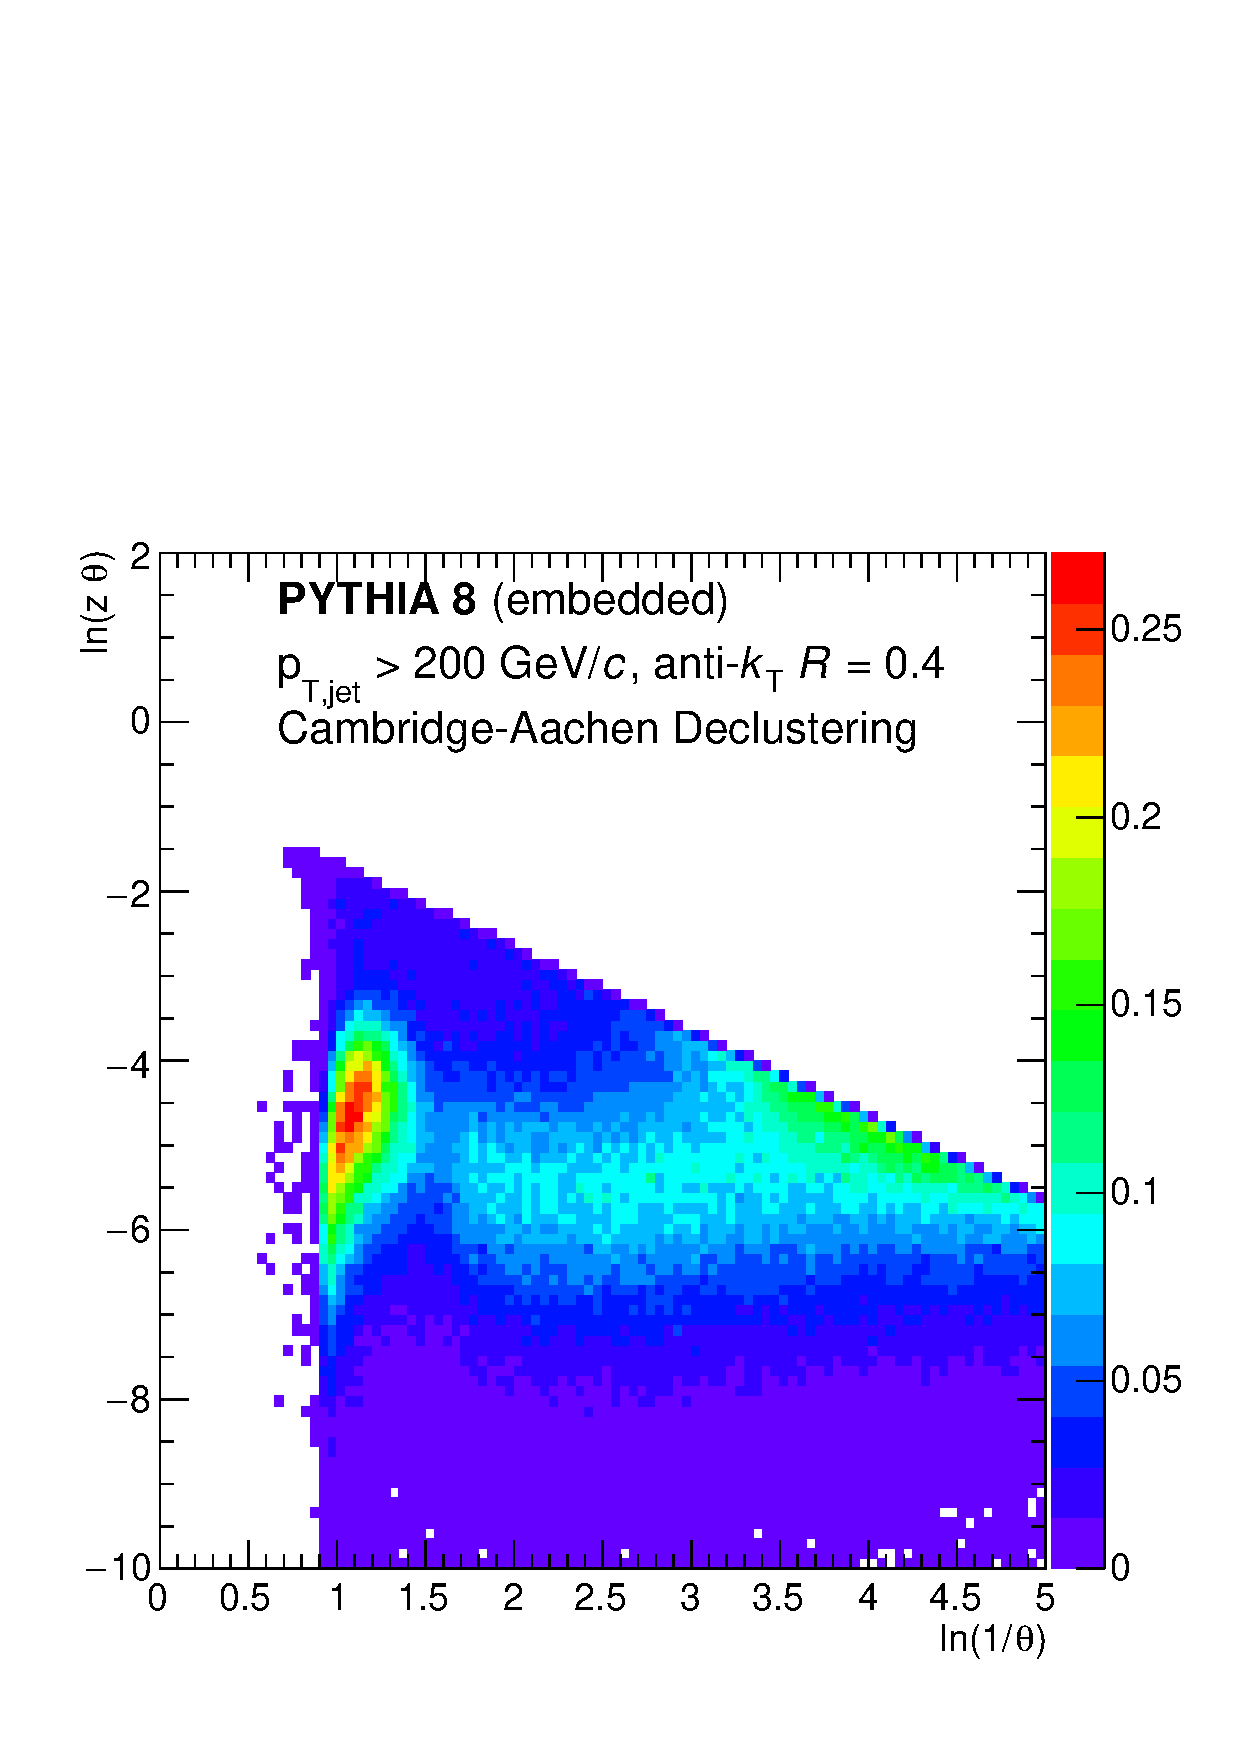
\includegraphics[width=0.33\textwidth]
{figures/LundMC/PythiaEmb_CA}%
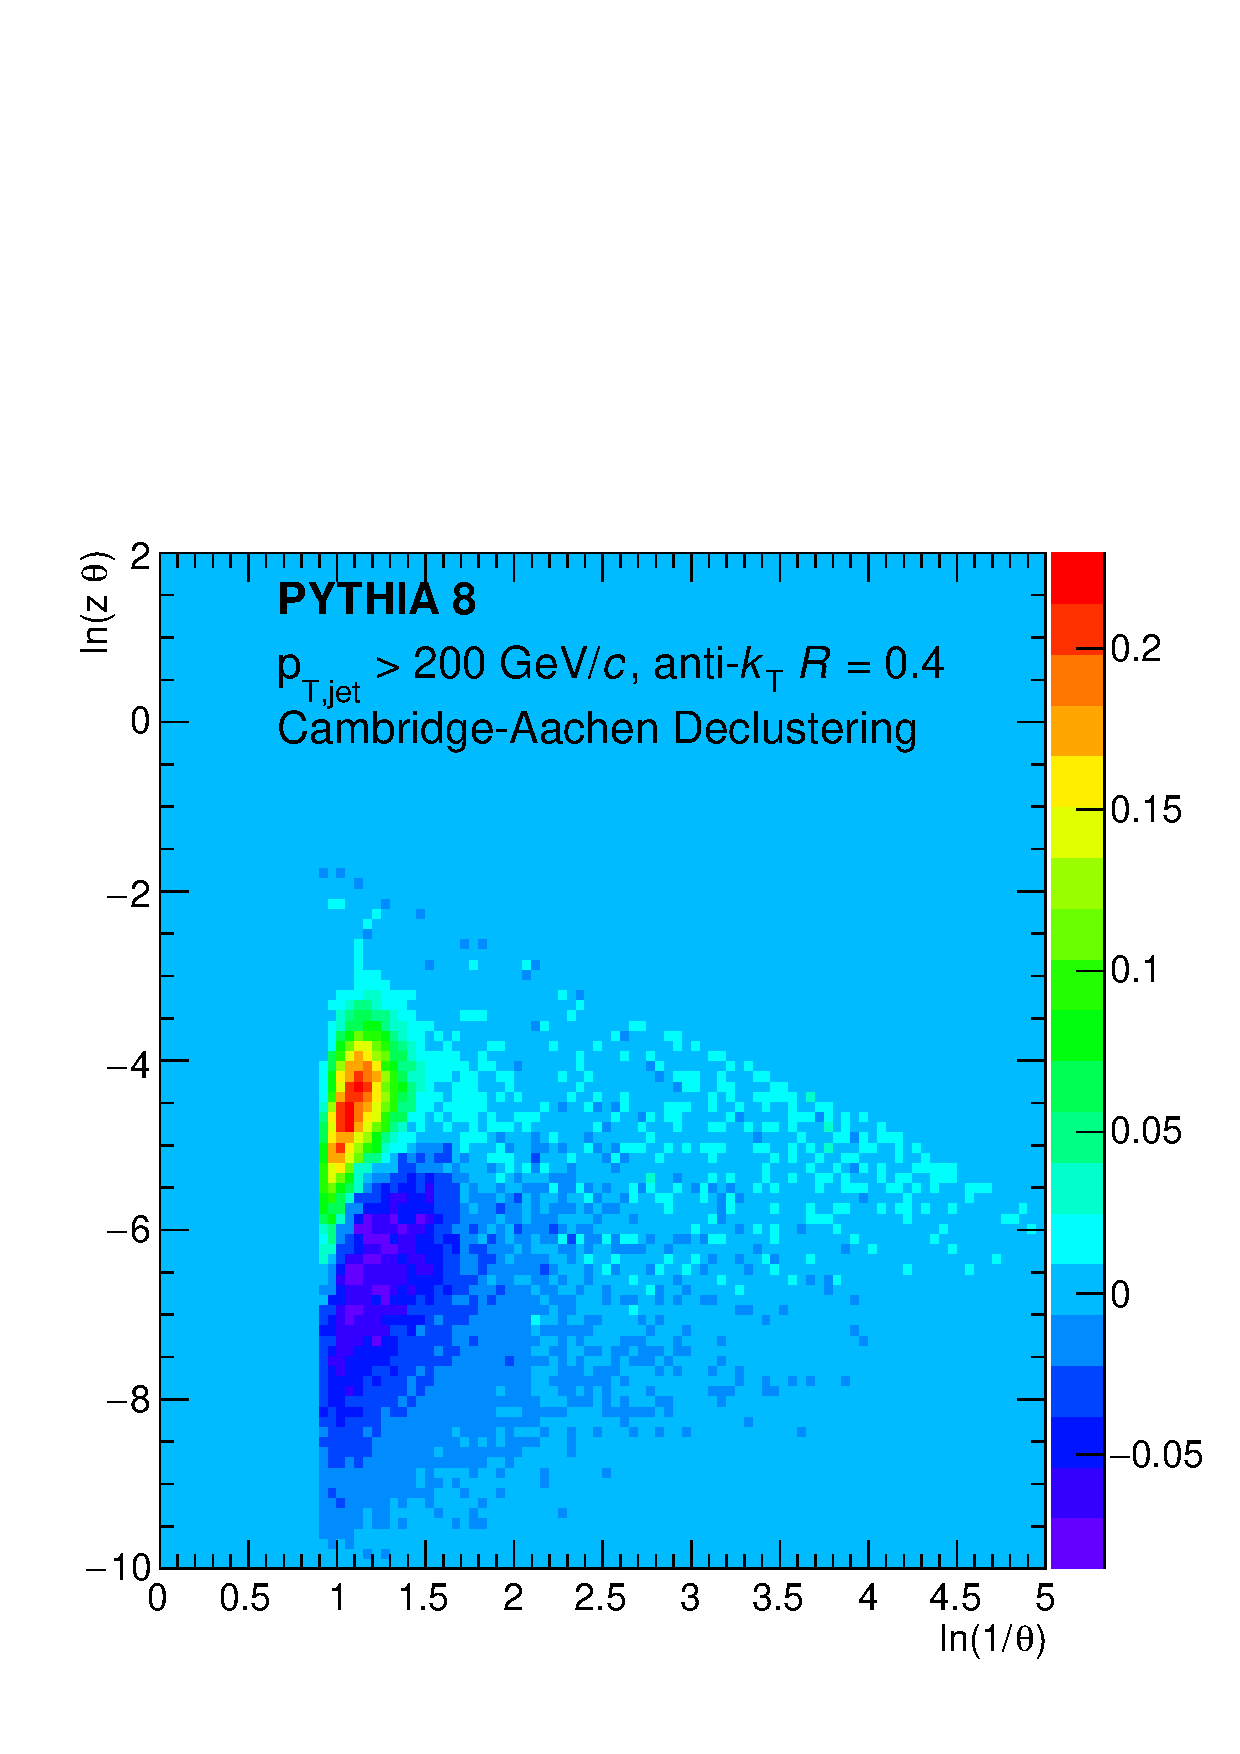
\includegraphics[width=0.33\textwidth]
{figures/LundMC/PythiaDiff_CA}%
\caption{Impact of the uncorrelated background in the splitting map of the PYTHIA shower.}
\label{fig:UncorrelatedBkg}
\end{figure}
%%%%%%%%%%%%%%%%%%%%%%%%%%%%%%%%%%%%%%%%

In all the studies performed so far in this Section, we have not included the effect of considering a realistic heavy-ion background. In these studies, we have been using thermal events corresponding to a momentum density of $\rho =120$ GeV which corresponds to the most central events in the CMS detector, corresponding to a total multiplicity of $\sim 7000$ particles. 
{\color{red} More details on background, where do we take it from, parameters,  referecens etc.. Details on embedding...}

Hence, ending this section, we would also like to point out the fragility of using the Lund kinematical diagram in a realistic, noisy environment.
The heavy ion background that is uncorrelated to the jet will populate the phase space in the form of soft splittings at large angle $\theta \sim R$, where the area is maximal. Depending on the considered jet $p_{T}$, these fake splittings can contribute significantly to the distribution of groomed observables, cf. \autoref{sec:jetsubstructure}, by enhancing the number of asymmetric splittings and inducing a strong modification relative to vacuum jets. 
\autoref{fig:UncorrelatedBkg} shows the Lund diagram filled iteratively with PYTHIA jets embedded into a thermal background (left) and the difference plot to PYTHIA (right). The difference plot shows the enhancement of uncorrelated splittings at large angles. 
%Superimposed to the plot, the black line with negative slope sets the limits for the subsample of splittings that would be selected by grooming with default parameters and highlights the fraction of fake splittings that would enter the $z_{g}$ calculation. The plot on the right is filled with jets at lower energies and shows that the impact of the uncorrelated background increases as expected.
This provides a hint that, no matter the grooming settings, this becomes a significant contribution to the observable the smaller the $\pT$.

%%%%%%%%%%%%%%%%%%%%%%%%%%%%%%%%%%%%%%%%
\begin{figure}
\centering
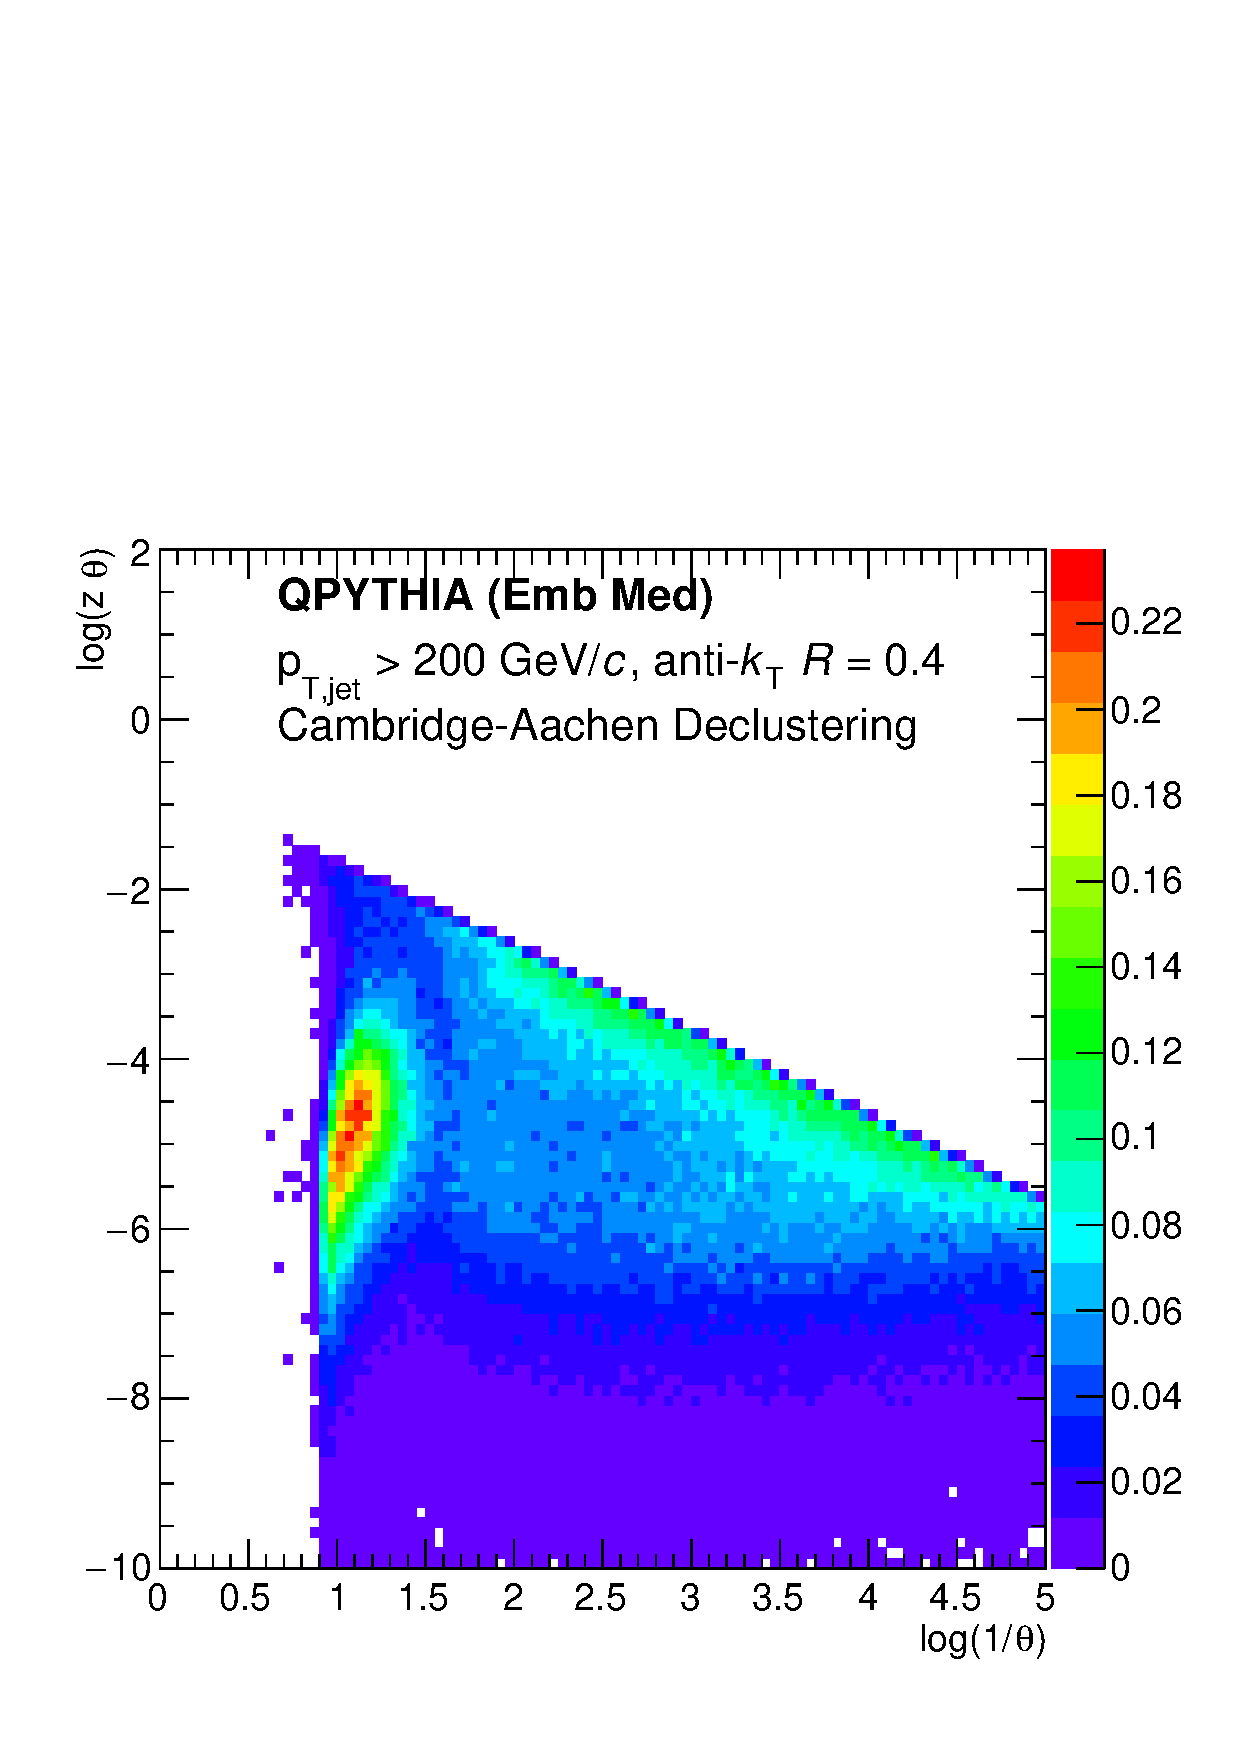
\includegraphics[width=0.32\textwidth]
{figures/LundMC/QPythiaEmbedded}
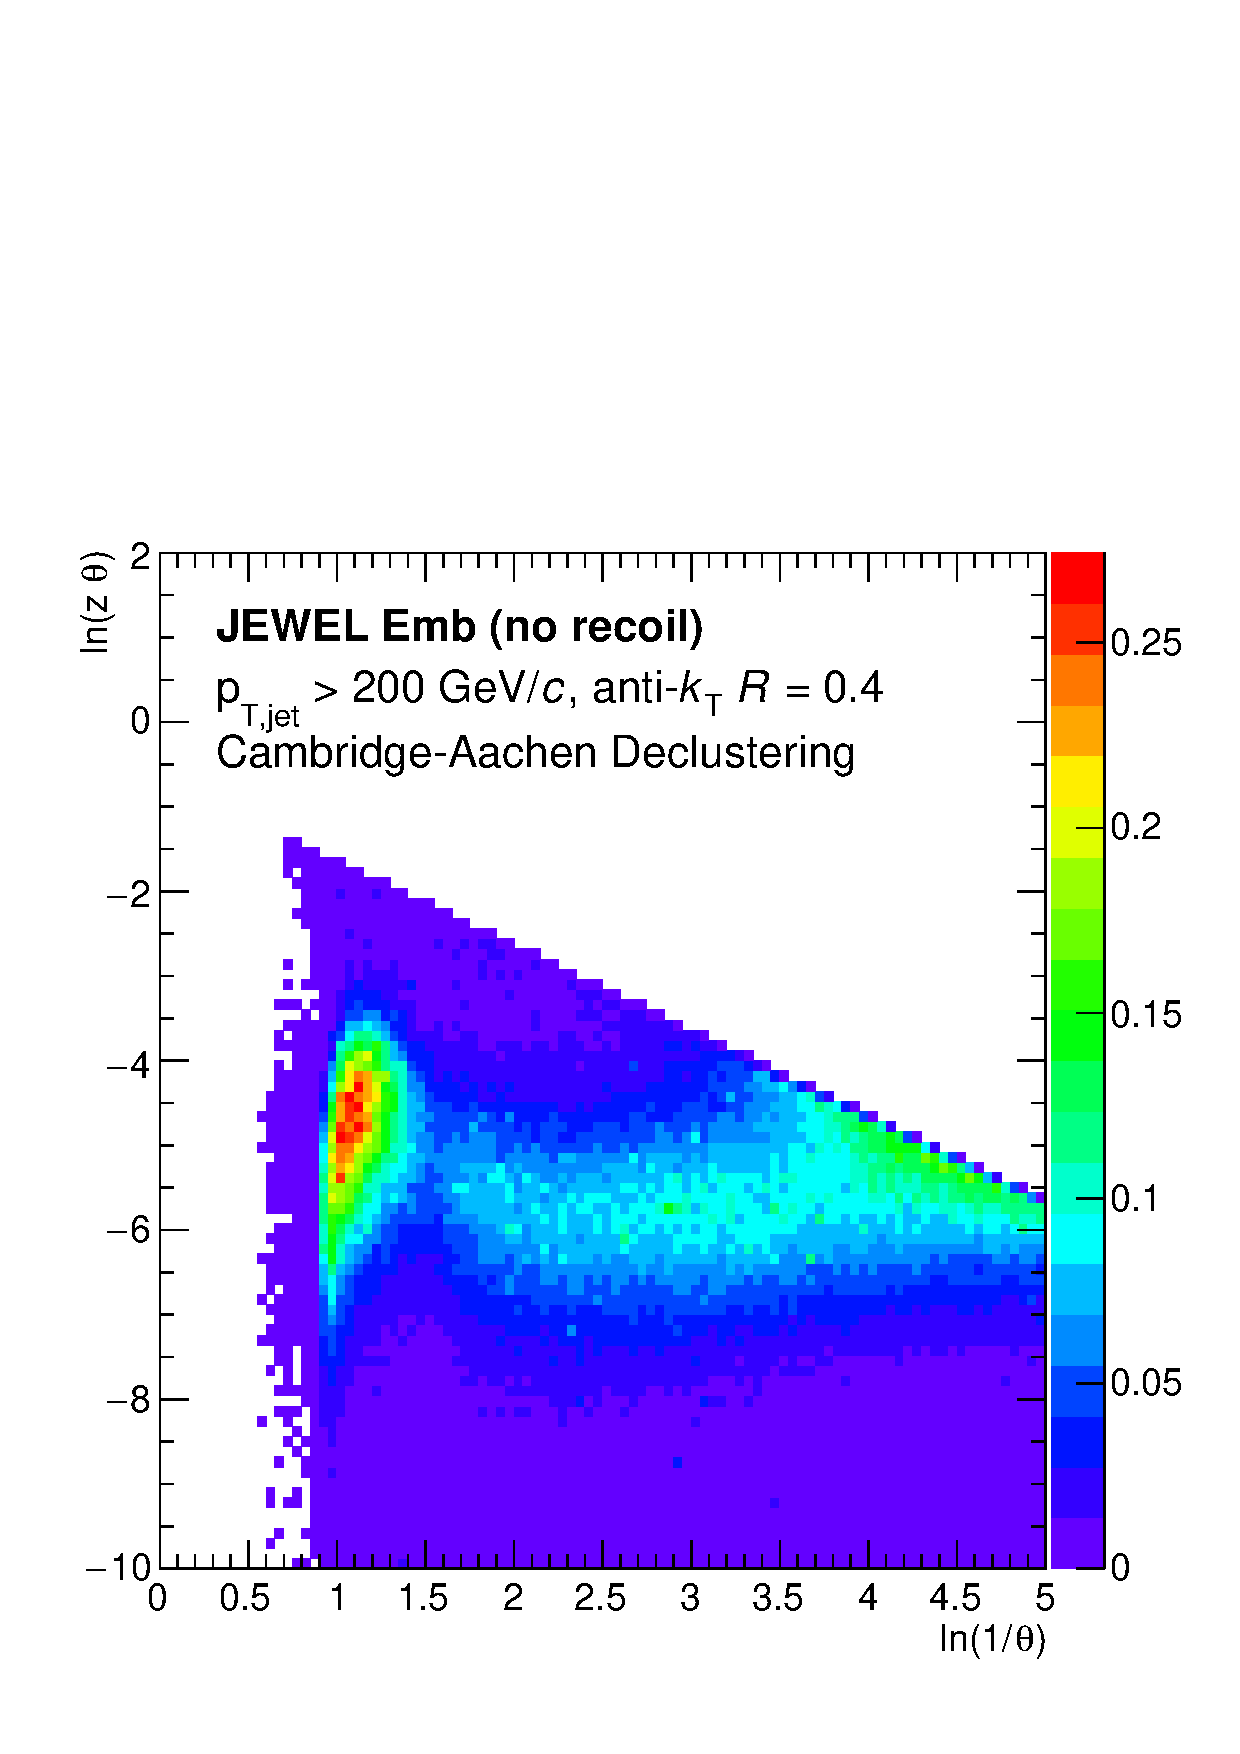
\includegraphics[width=0.32\textwidth]
{figures/LundMC/Jewel_MedEmb_RecoilOff}
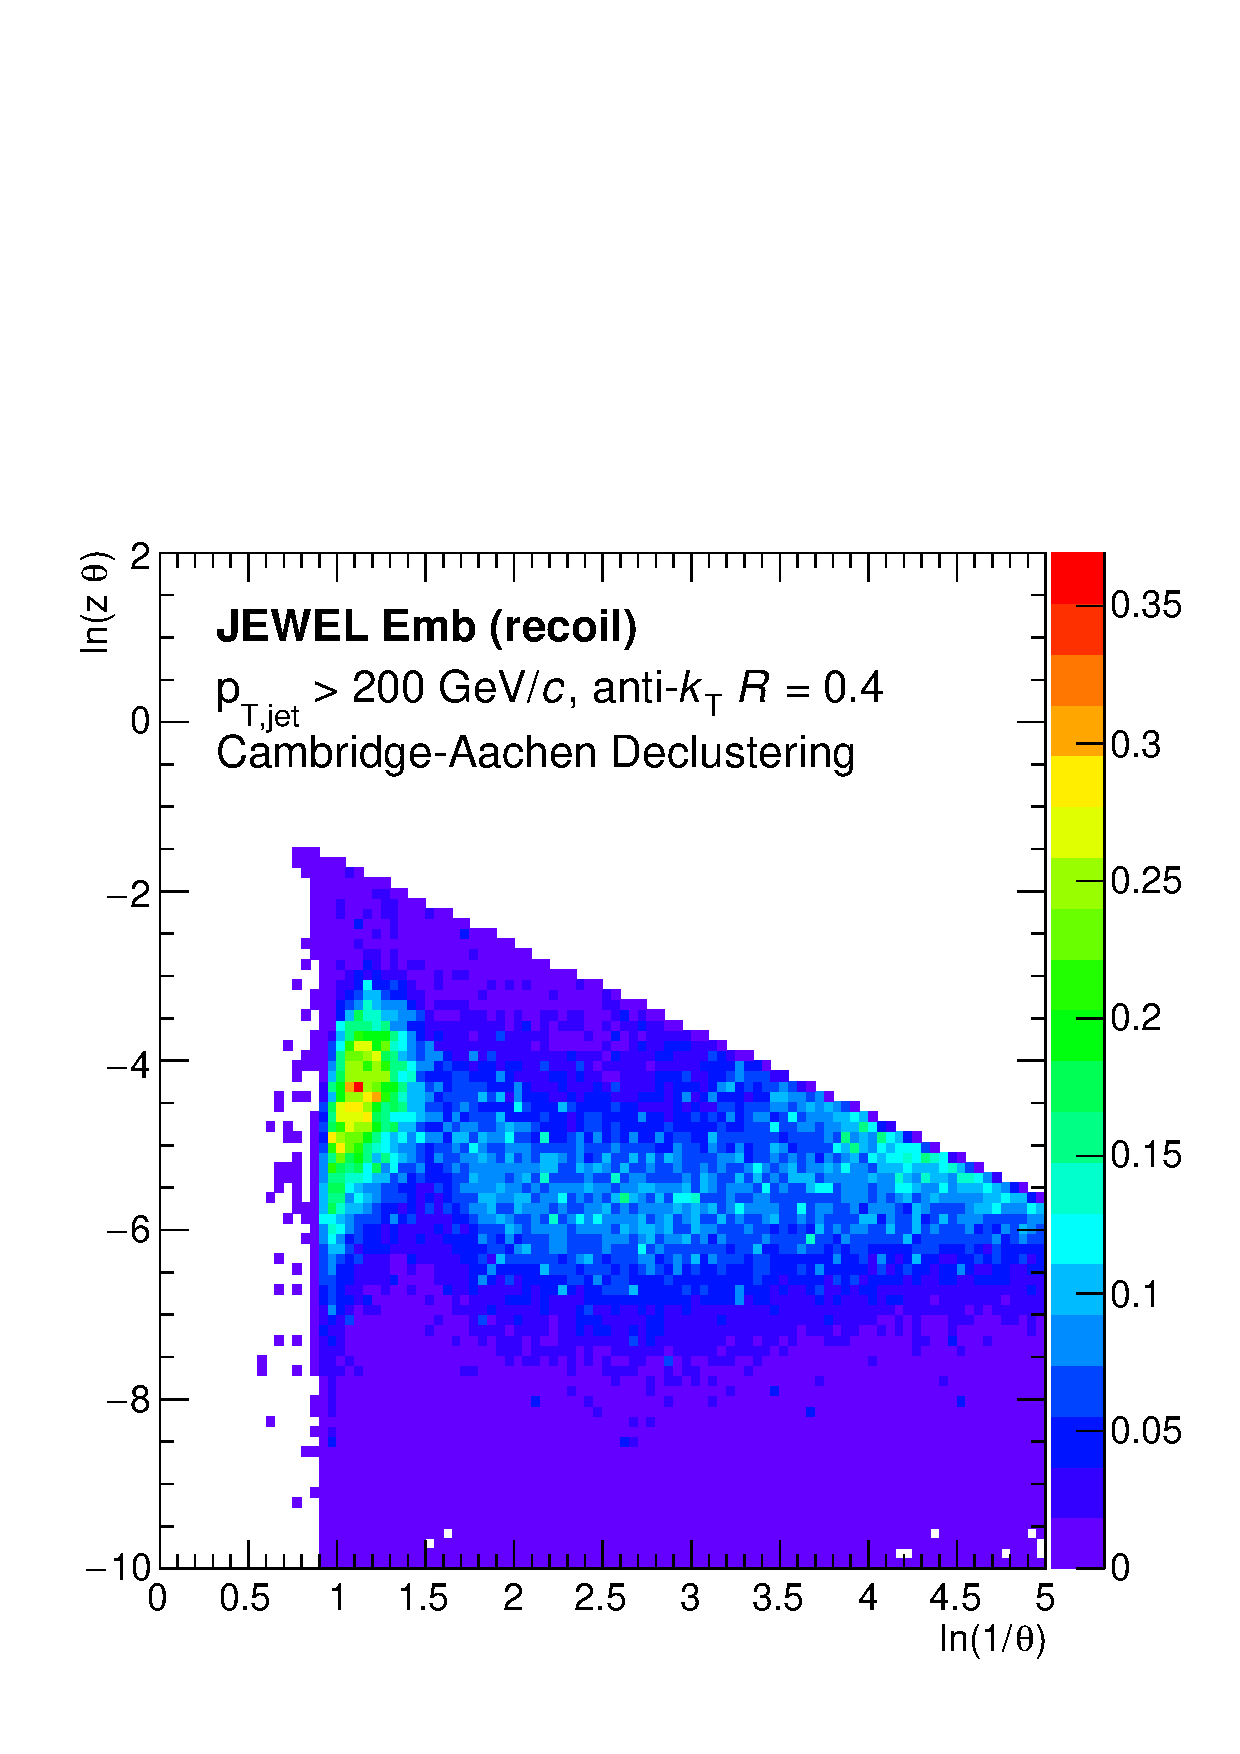
\includegraphics[width=0.32\textwidth]
{figures/LundMC/Jewel_MedEmb_}\\
%\includegraphics[width=0.32\textwidth]
%{figures/LundMC/QPythiaEmbeddedDiff}
%\includegraphics[width=0.32\textwidth]
%{figures/LundMC/Jewel_EmbDiff_RecoilOff}
%\includegraphics[width=0.32\textwidth]
%{figures/LundMC/Jewel_EmbDiff_}
\caption{Impact of the uncorrelated background in the splitting map of the medium parton showers QPYTHIA and JEWEL. Upper row shows the resulting splitting map when embedding the modeled showers in a background. 
%Lower row shows the difference of the showers with and without embedding.
}
\label{fig:UncorrelatedBkgSignal}
\end{figure}
%%%%%%%%%%%%%%%%%%%%%%%%%%%%%%%%%%%%%%%%
As expected, this a prominent feature for the in-medium showers as well.
Similar plots are shown for QPYTHIA and JEWEL embedded showers are shown in \autoref{fig:UncorrelatedBkgSignal}. The upper row correspond to QPYTHIA, JEWEL ``Recoils Off'' and JEWEL ``Recoils on'' embedded onto a thermal background. 
%The lower plot show the difference of the splitting map before and after embedding. 
Strikingly, all three plots share a similar dominant feature at large angles. This is confirmed by subtracting the generator-level events from the embedded ones. However, we observe that after embedding, the difference to the vacuum reference (also embedded) is still significant, meaning that the differences in the fragmentation pattern from different generators survive the presence of an underlying event, albeit with significant distortions.

%!TEX root = THinstituteReport_1.tex

%%%%%%%%%%%%%%%%%%%%%%%%%%%%%%%%%%%%%%%%%
\section{Jet substructure}
\label{sec:jetsubstructure}
%%%%%%%%%%%%%%%%%%%%%%%%%%%%%%%%%%%%%%%%%

As mentioned before, jet substructure techniques usually involve a step which reorganizes the constituents of a jet into a hierarchical tree where the nodes represent subsequent splitting processes.
This structure serves for further analysis using additional techniques called jet grooming and tagging algorithms.
Grooming techniques usually reorganizes the tree by discarding radiation that fail to pass given criteria, corresponding typically to soft and large-angle radiation. Taggers, on the other hand, aim at identifying the first splitting that passes a given criterion. In this way it splits a jet into two sub-jets. There has been a lot of progress recently utilizing these techniques for a wide range of substructure observables \cite{Butterworth:2008iy,Ellis:2009me,Krohn:2009th,Dasgupta:2013ihk,Larkoski:2014wba}, for a recent review see e.g. \cite{Larkoski:2017jix}. At least within the C/A algorithm, the subjets identified using grooming are in close correspondence to 
%access to the properties of 
the first splitting of the parton evolution in the vacuum~\cite{Altarelli:1977zs,Larkoski:2015lea}.

While medium-modified jet fragmentation functions and other jet shape observables have been studied experimentally since many years, only recently have these techniques been applied in the context of heavy-ion collisions.
Jet grooming was recently introduced as a tool to study the medium modification of leading partonic components in a parton shower~\cite{Sirunyan:2017bsd}, for related theoretical interpretations see \cite{Chien:2016led,Mehtar-Tani:2016aco,Milhano:2017nzm,Chang:2017gkt}. 
%Jet grooming algorithms are used to split a single jet into two subjets, a process referred to as ``declustering''~. 

Given the proliferation of existing techniques, we will only refer to these as grooming techniques and concretely study one within the scope of this report, namely the Soft Drop procedure.
The Soft Drop algorithm reclusters the anti-$k_{\mathrm{T}}$ jet constituents using C/A to create an angular-ordered clustering tree. On this tree a pairwise declustering is performed. In each step of the declustering the softer branch is removed until a branch is found that satisfies
%\begin{linenomath}
\beq
\label{eq:groompar}
\frac{\mathrm{min}(p_{\mathrm{T},i},p_{\mathrm{T},j})}{p_{\mathrm{T},i}+p_{\mathrm{T},j}} > z_{\text{cut}}\left( \frac{\Delta R_{ij}}{R_{0}} \right)^{\beta},
\eeq
%\end{linenomath}
where the subscripts ``$i$'' and ``$j$'' indicate the subjets at that step of the declustering, $\Delta R_{ij}$ is the distance between the two subjets, $R_{0}$ is the cone size of the anti-$k_{\mathrm{T}}$ jet, and $z_{\text{cut}}$ and $\beta$ are adjustable parameters. By varying $z_{\text{cut}}$ and $\beta$, specific regions of the emission phase space, see \autoref{fig:PS1}, can be isolated. For $\beta = 0$, this procedure is identical to the modified mass-drop tagger \cite{Dasgupta:2013ihk}, while $\beta \neq 0$ was introduced in \cite{Larkoski:2014wba}. It allows to design specific grooming settings sensitive to distinct regions of the kinematical phase space represented in the Lund plane. Equivalently, the parameters can be adjusted to suppress or enhance the effect of medium modifications.
%, for example, to semi-hard radiation from single hard scatterings, soft radiation in the BDMPS regime and soft contribution originating from heating up the medium while the parton shower traverses it.

%%%%%%%%%%%%%%%%%%%%%%%%%%%%%%%%%%%%%
\begin{figure}[t!]
\centering
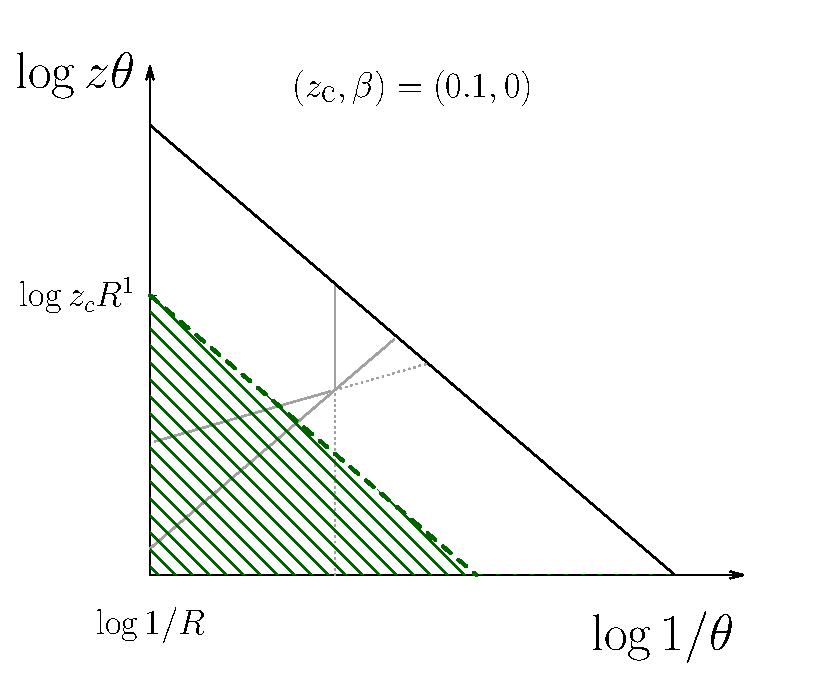
\includegraphics[width=0.33\textwidth]{figures/kinematics/plotVac_SD2_2}%
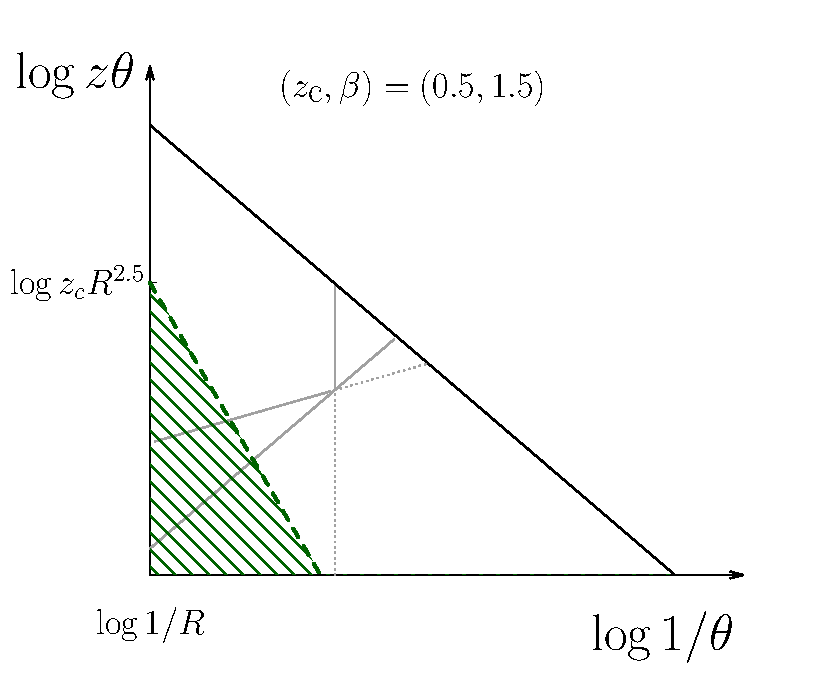
\includegraphics[width=0.33\textwidth]{figures/kinematics/plotVac_SD1_2}%
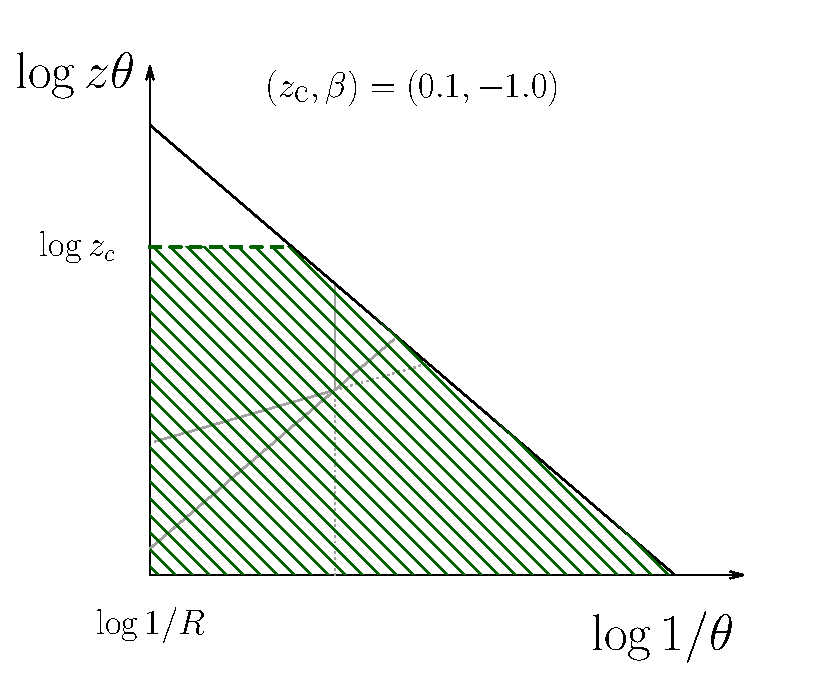
\includegraphics[width=0.33\textwidth]{figures/kinematics/plotVac_SD3_2}%
\caption{The three grooming settings studied in this report, see text for details. Shaded areas correspond to configuration that are groomed away.}
\label{fig:TheorySD}
\end{figure}
%%%%%%%%%%%%%%%%%%%%%%%%%%%%%%%%%%%%%
In this report, we compare the three grooming settings:
\begin{description}
\item[{\bf SD1:}] $z_{\text{cut}}=0.1$ and $\beta=0$: removes branches based only on the energy fraction;
\item[{\bf SD2:}]  $z_{\text{cut}}=0.5$ and $\beta=1.5$: has a stronger grooming at large angle;
\item[{\bf SD3:}]  $z_{\text{cut}}=0.1$ and $\beta=-1.0$: selects only hard radiation;
\end{description}
\autoref{fig:TheorySD} depicts how these settings remove parts of the phase space in the Lund plane. This will in turn affect the demands on statistics, especially for the SD3 setting. While the first setting is the more widely used in various studies of the SD procedure, the two latter are designed to suppress regions of phase space with a lot of medium activity, as identified in the diagrams in \autoref{fig:PS2}. One could, of course, devise other grooming strategies, or even combine various conditions, in order to ``carve'' out kinematical regimes of particular interest. We avoid such prescriptions here in order not to bias our jet sample excessively. On the other hand, it could be interesting to combine grooming strategies with specific reclustering algorithms, a point we briefly study in \autoref{sec:hadronization}.
%{\color{red} some more description needed}

%\begin{figure}[h]
%\centering
%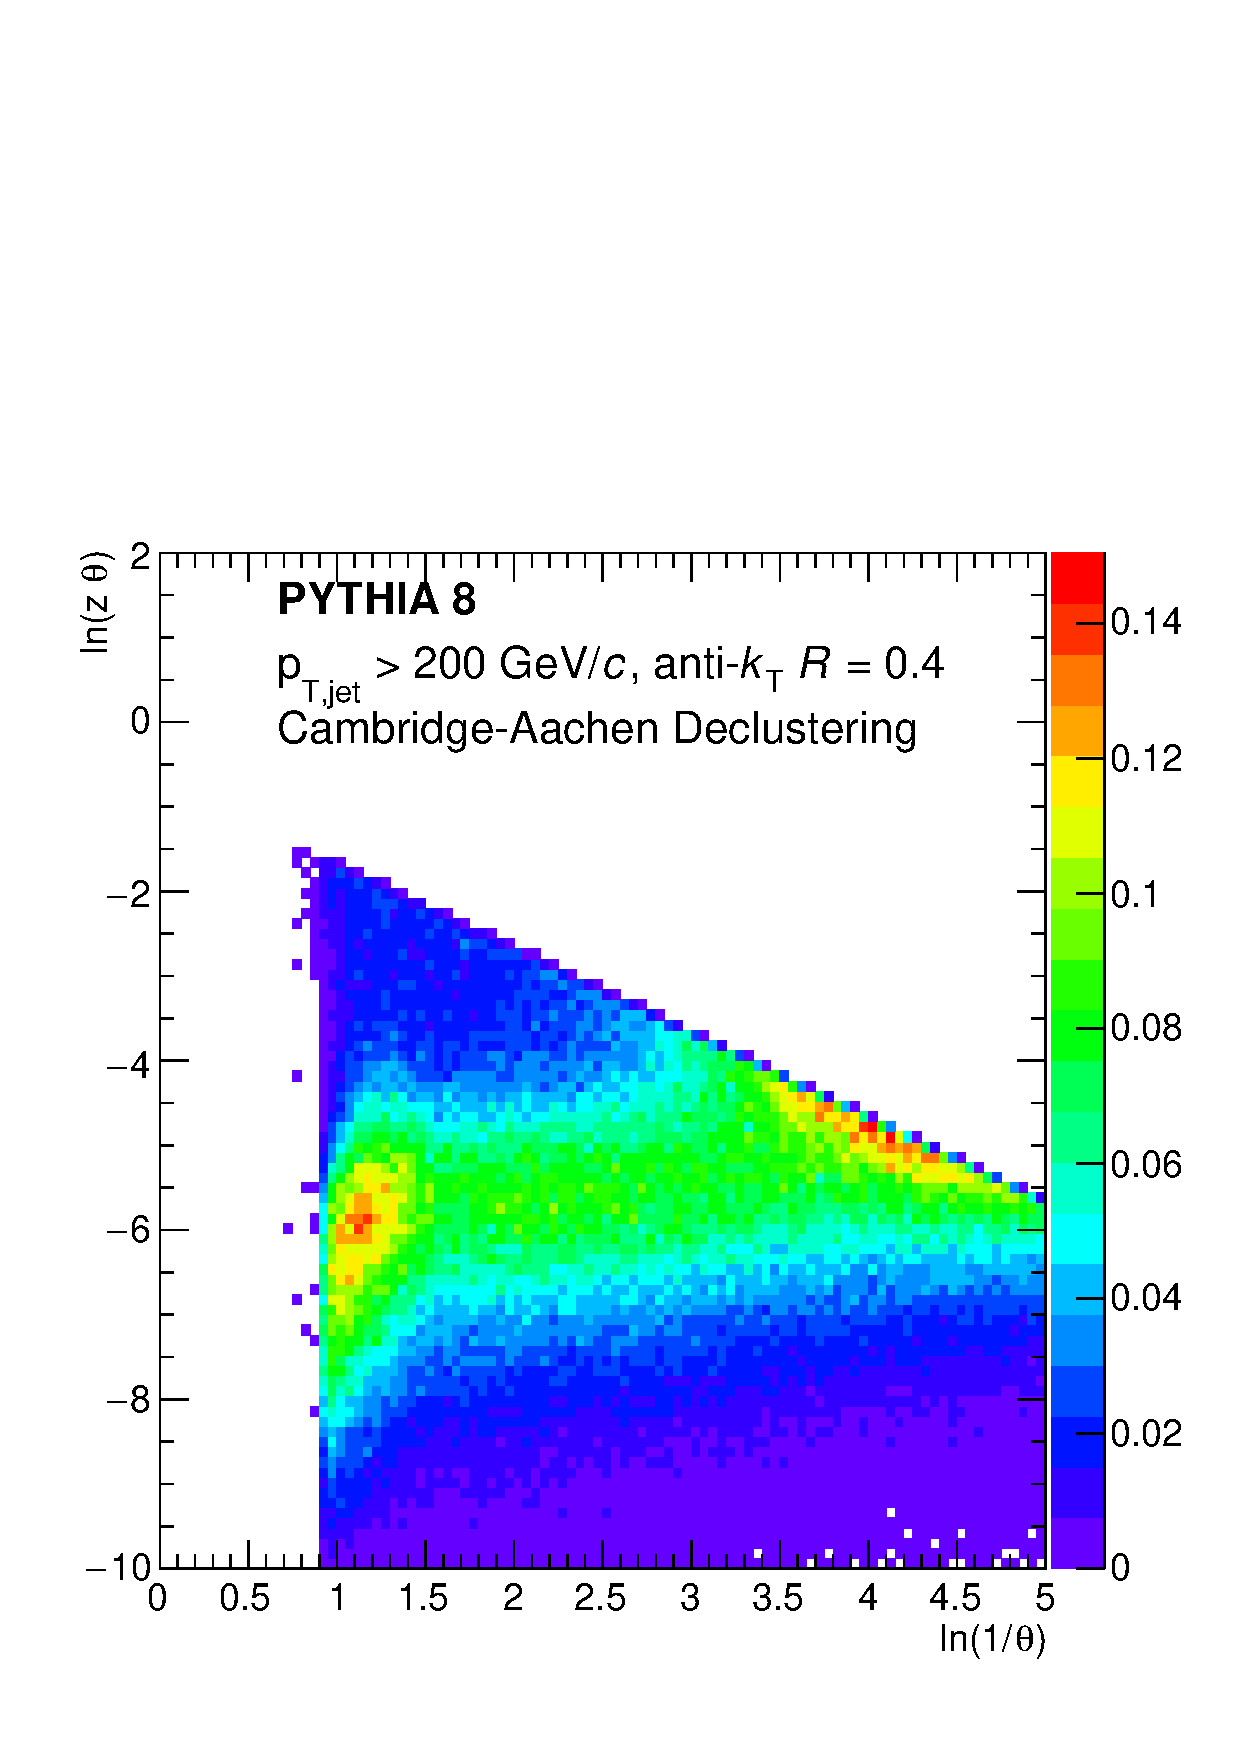
\includegraphics[width=0.33\textwidth]{figures/LundMC/Pythia_CA}
%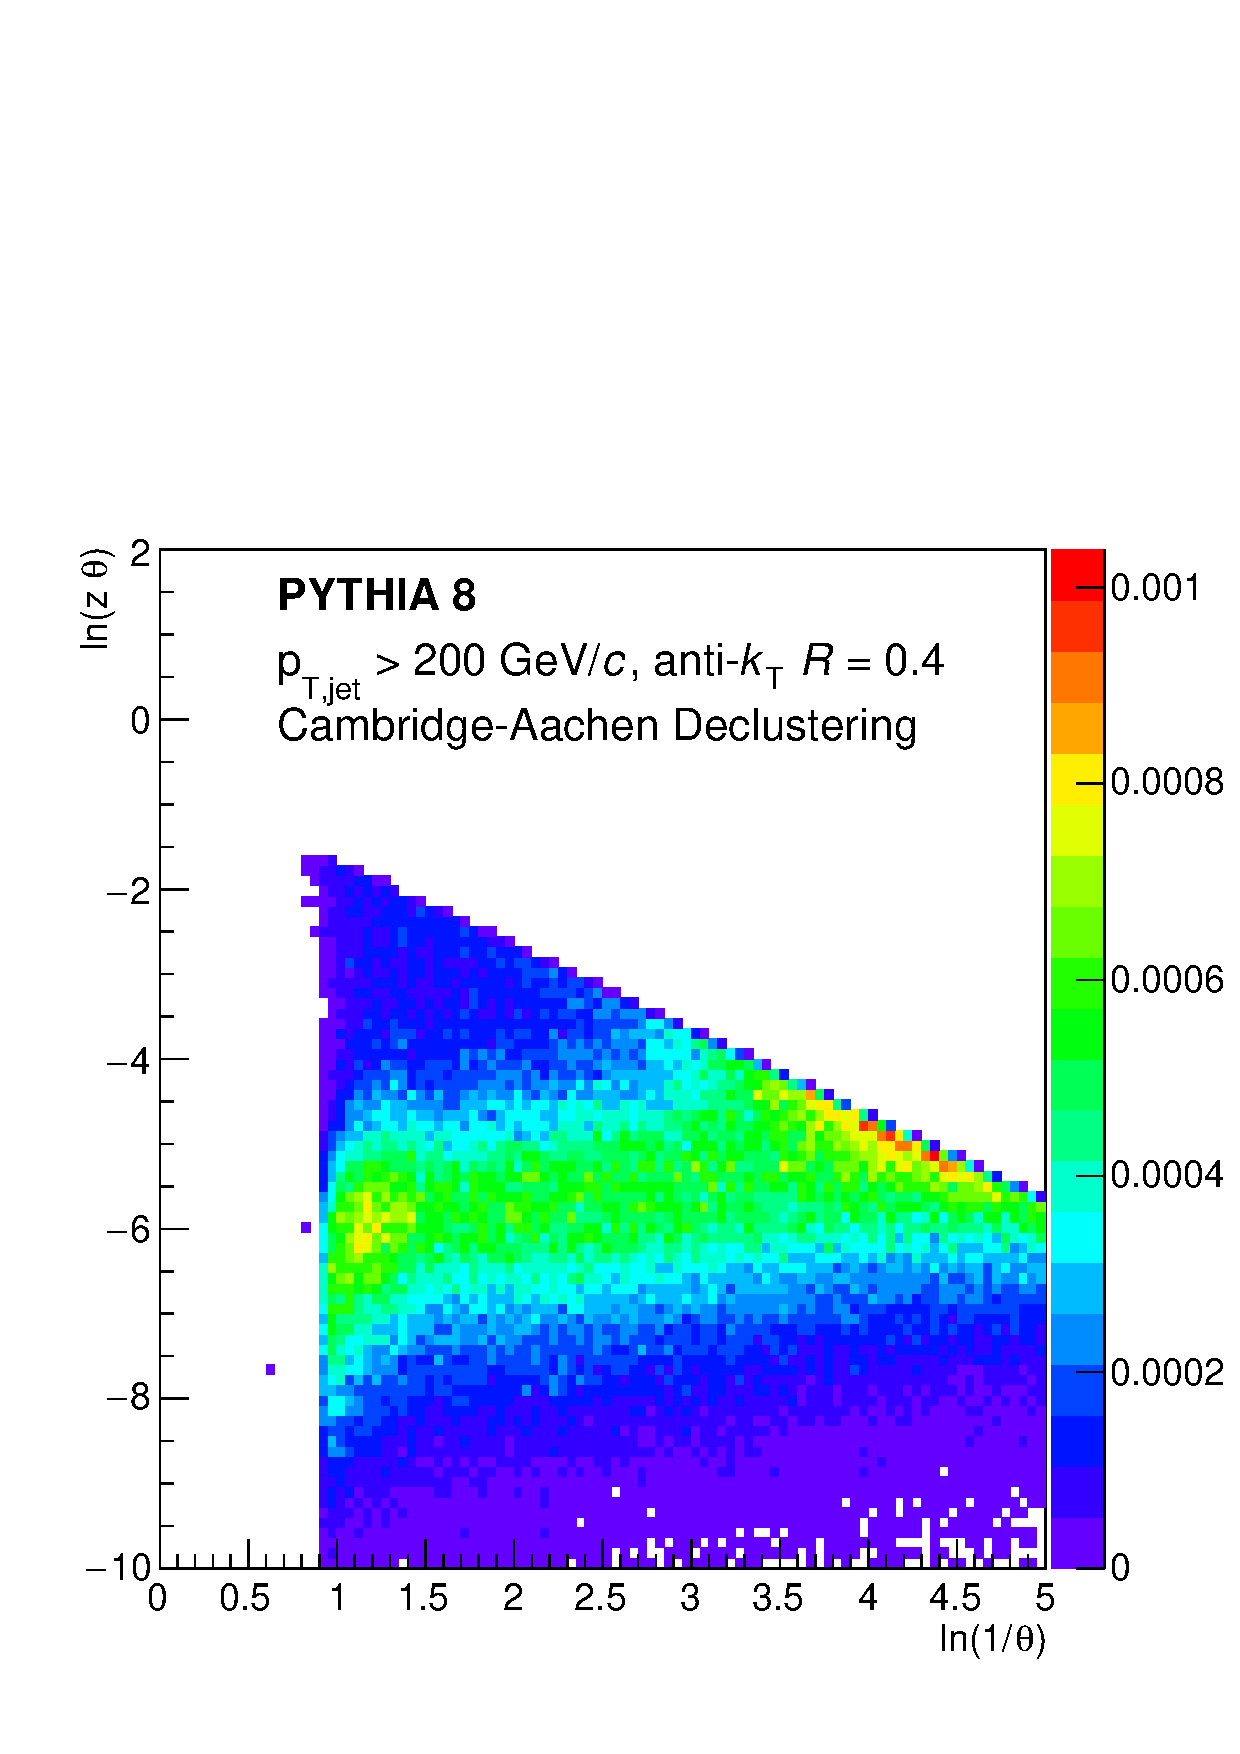
\includegraphics[width=0.33\textwidth]{figures/LundMC/Pythia_NoUE}
%\caption{Lund diagram reconstructed from jets generated by PYTHIA8 with (left) and without underlying event (right)}
%\label{fig:PS2Vac}
%\end{figure}
%introduce grooming; explaining clustering/declustering
%%%%%%%%%%%%%%%%%%%%%%%%%%%%%%%%%%%%%%%%%%%%%
%\subsection{Radiation phase space and sensitivity to jet quenching {\color{green} Leticia,Harry}}
%\label{sec:radiationPSJQ}
%%%%%%%%%%%%%%%%%%%%%%%%%%%%%%%%%%%%%%%%%%%%%
%\subsubsection{Medium-induced radiation}
%%%%%%%%%%%%%%%%%%%%%%%%%%%%%%%%%%%%%%
%\begin{figure}[h]
%\centering
%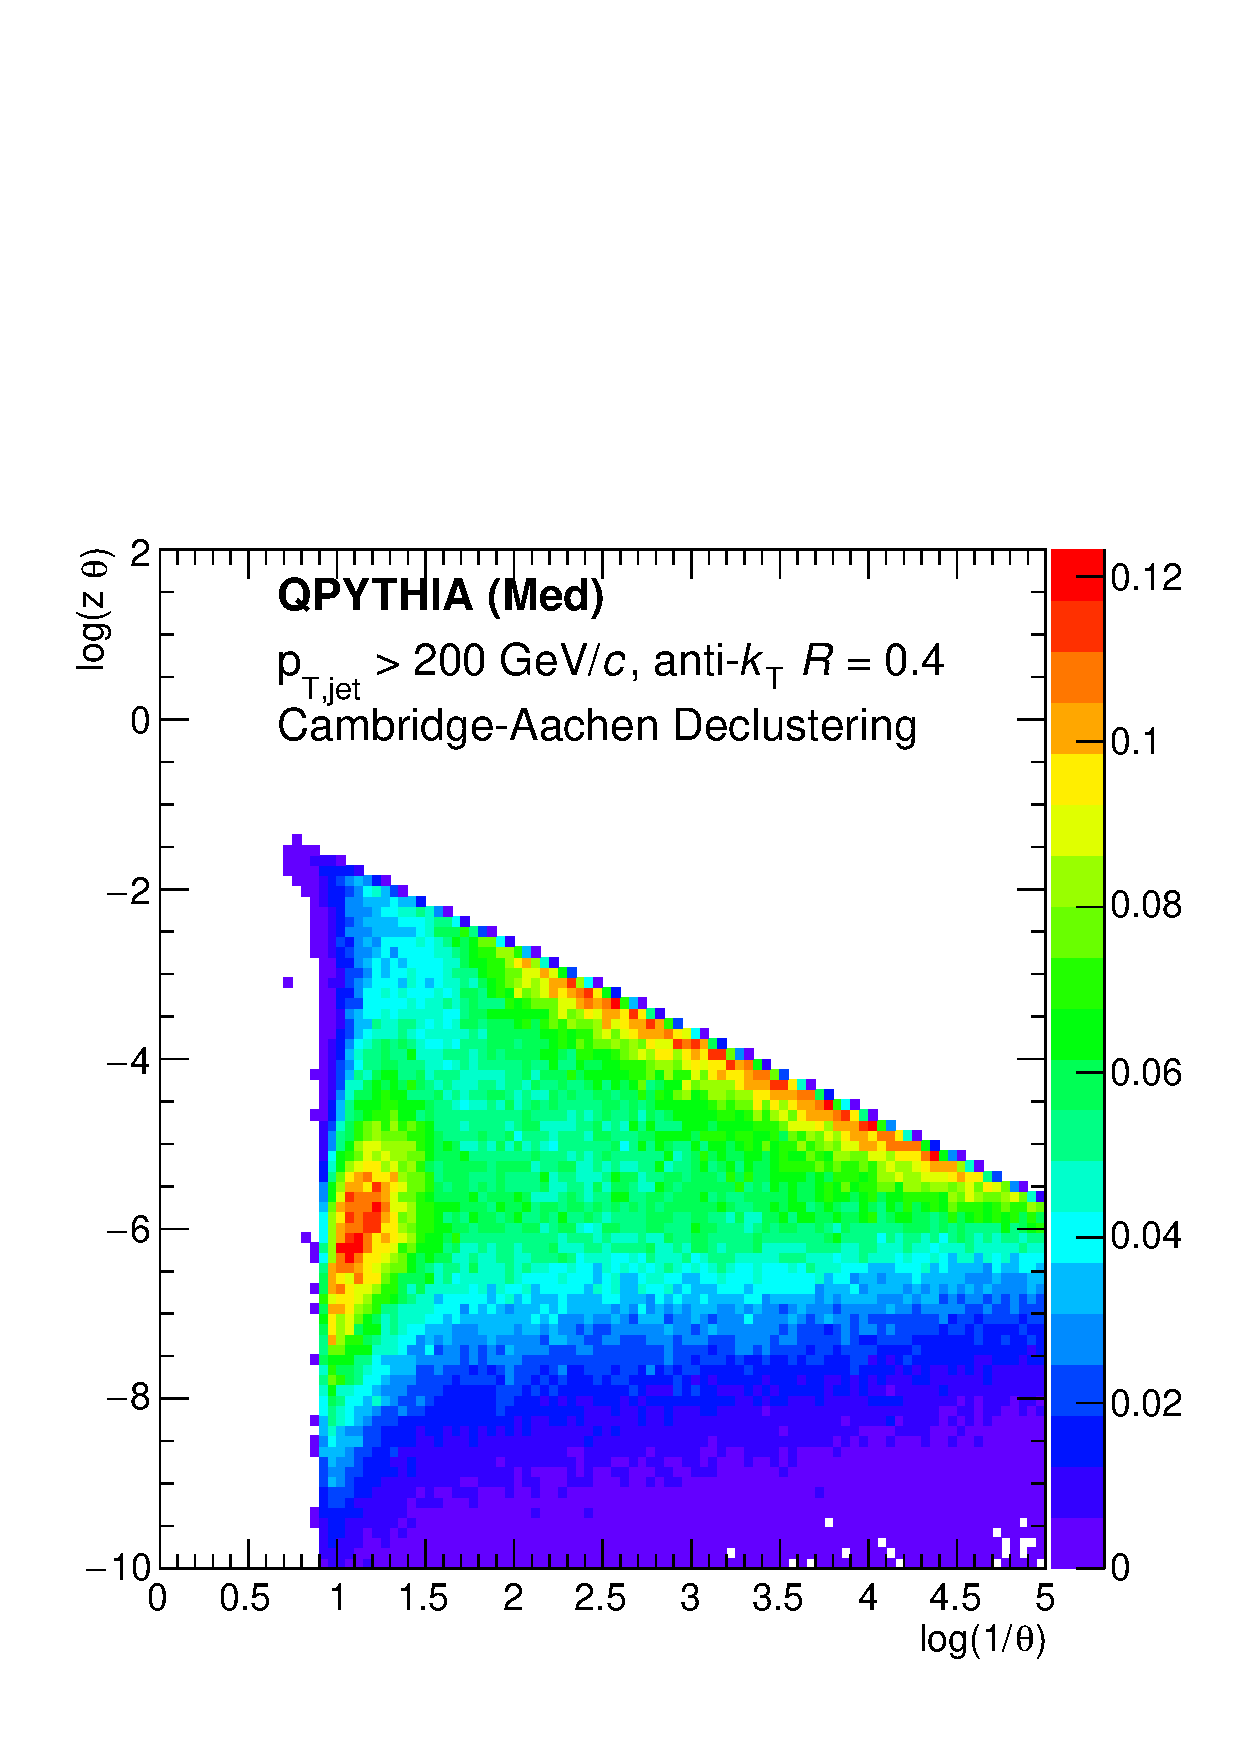
\includegraphics[width=0.3\textwidth]{figures/LundMC/QPythiaHyd200}
%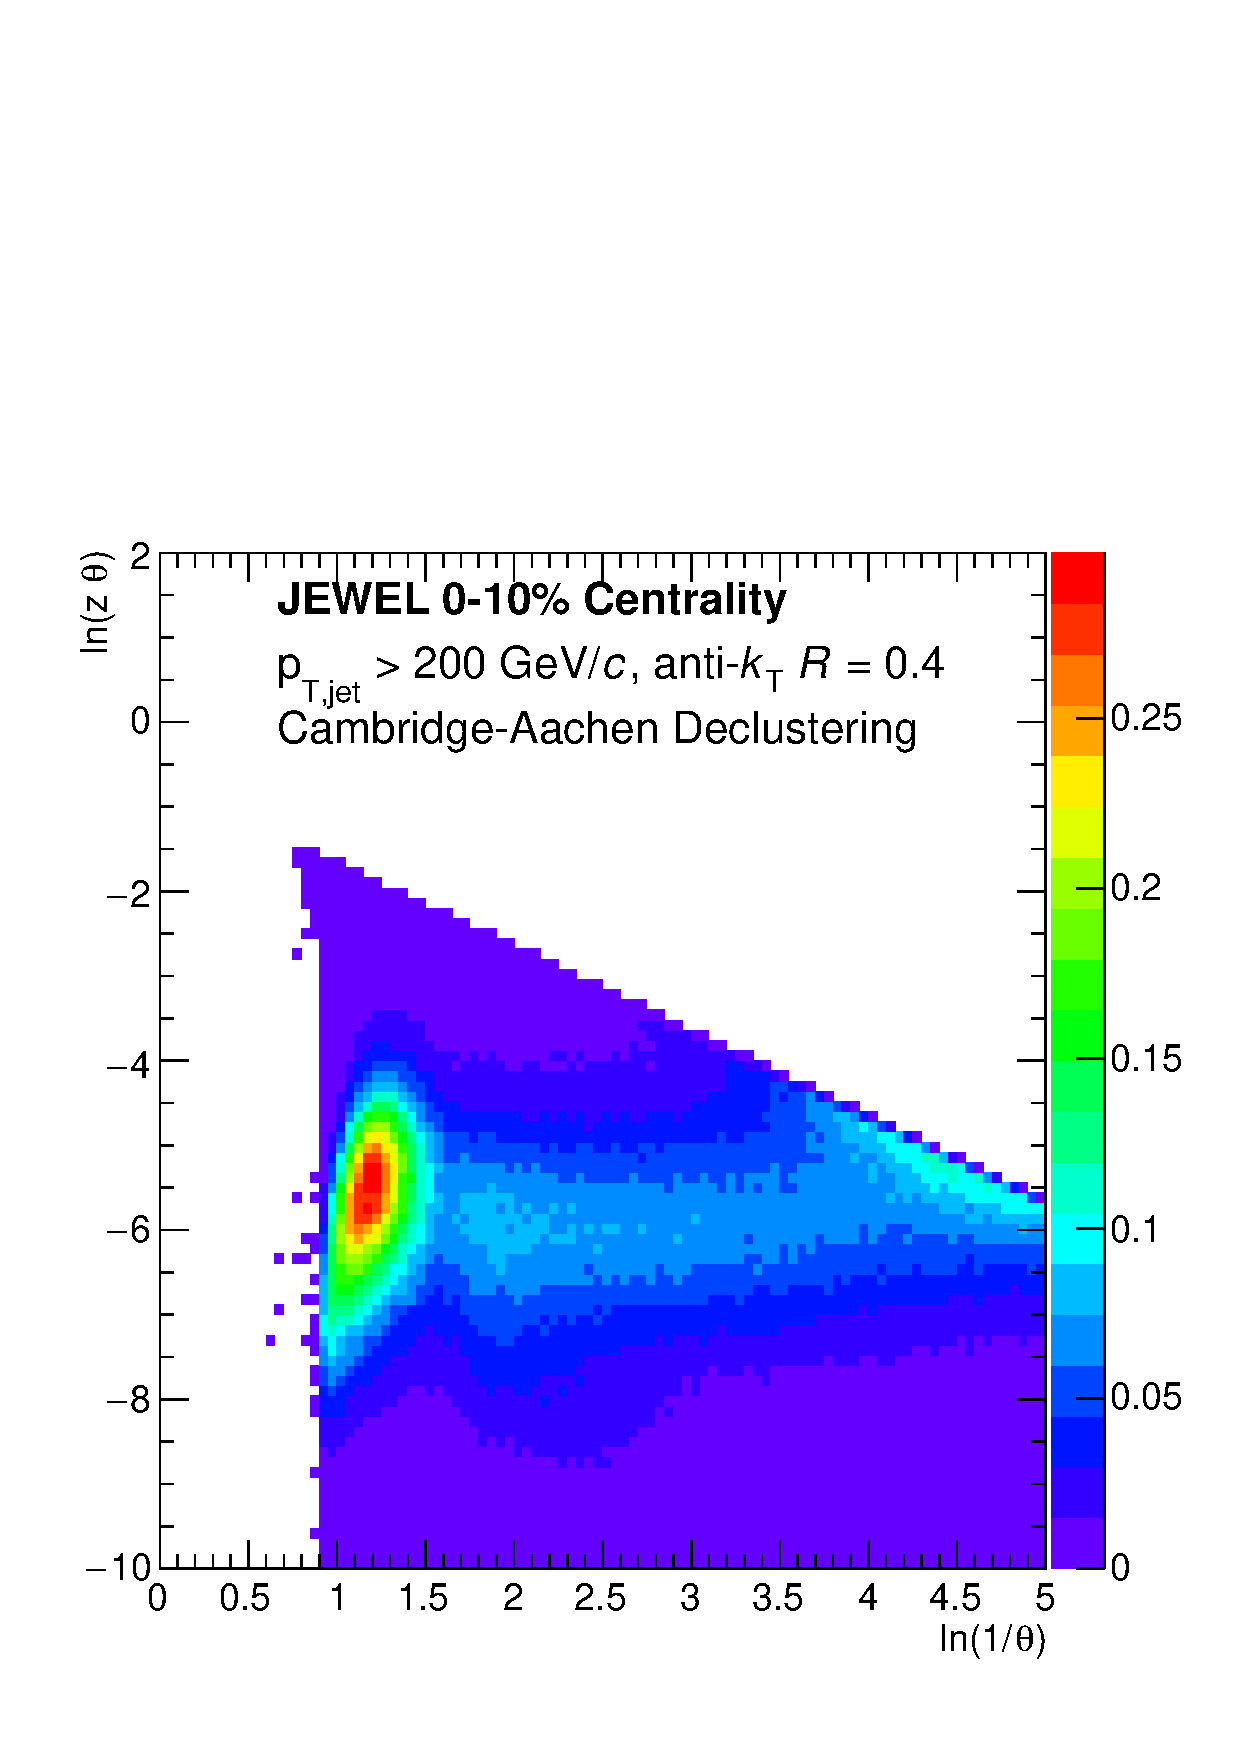
\includegraphics[width=0.3\textwidth]{figures/LundMC/JewelRecoilOff}
%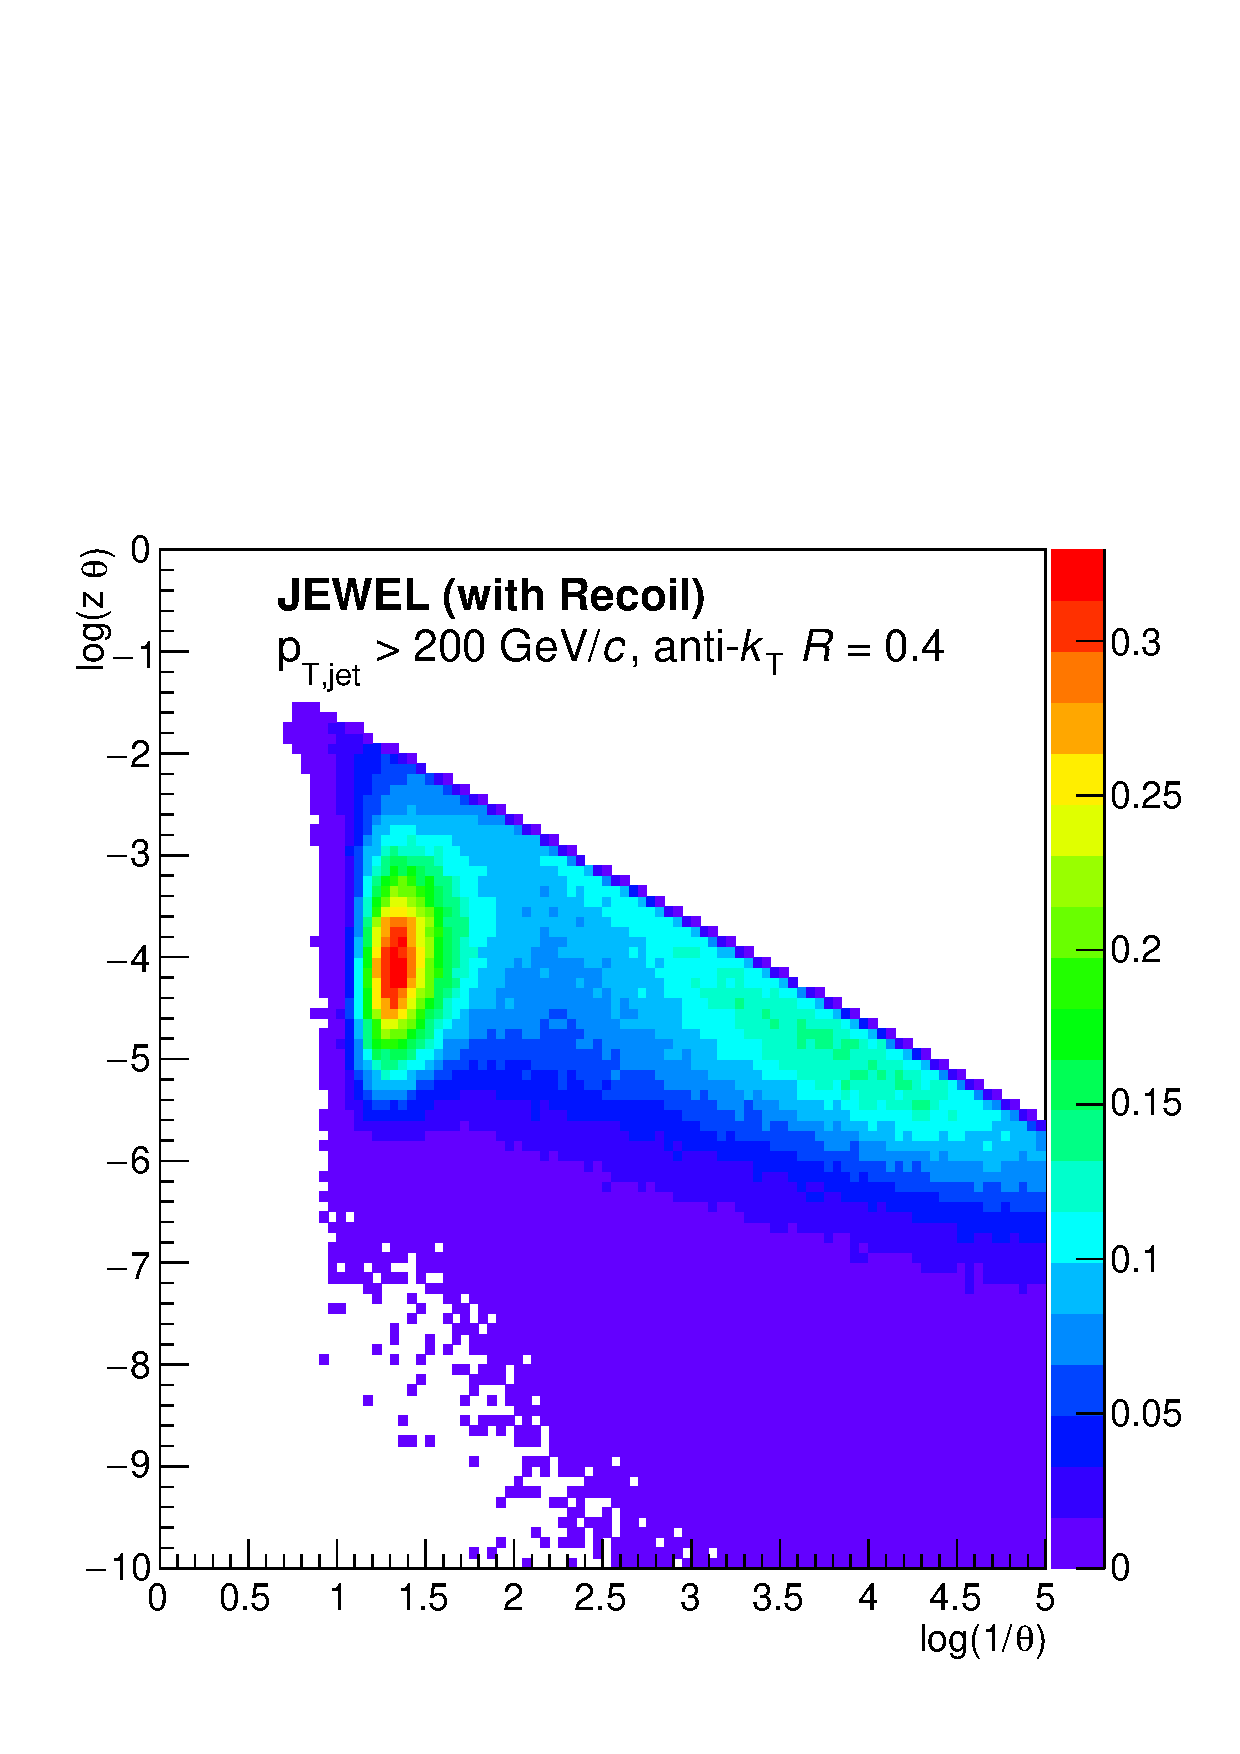
\includegraphics[width=0.3\textwidth]{figures/LundMC/JewelRecoilOn}
%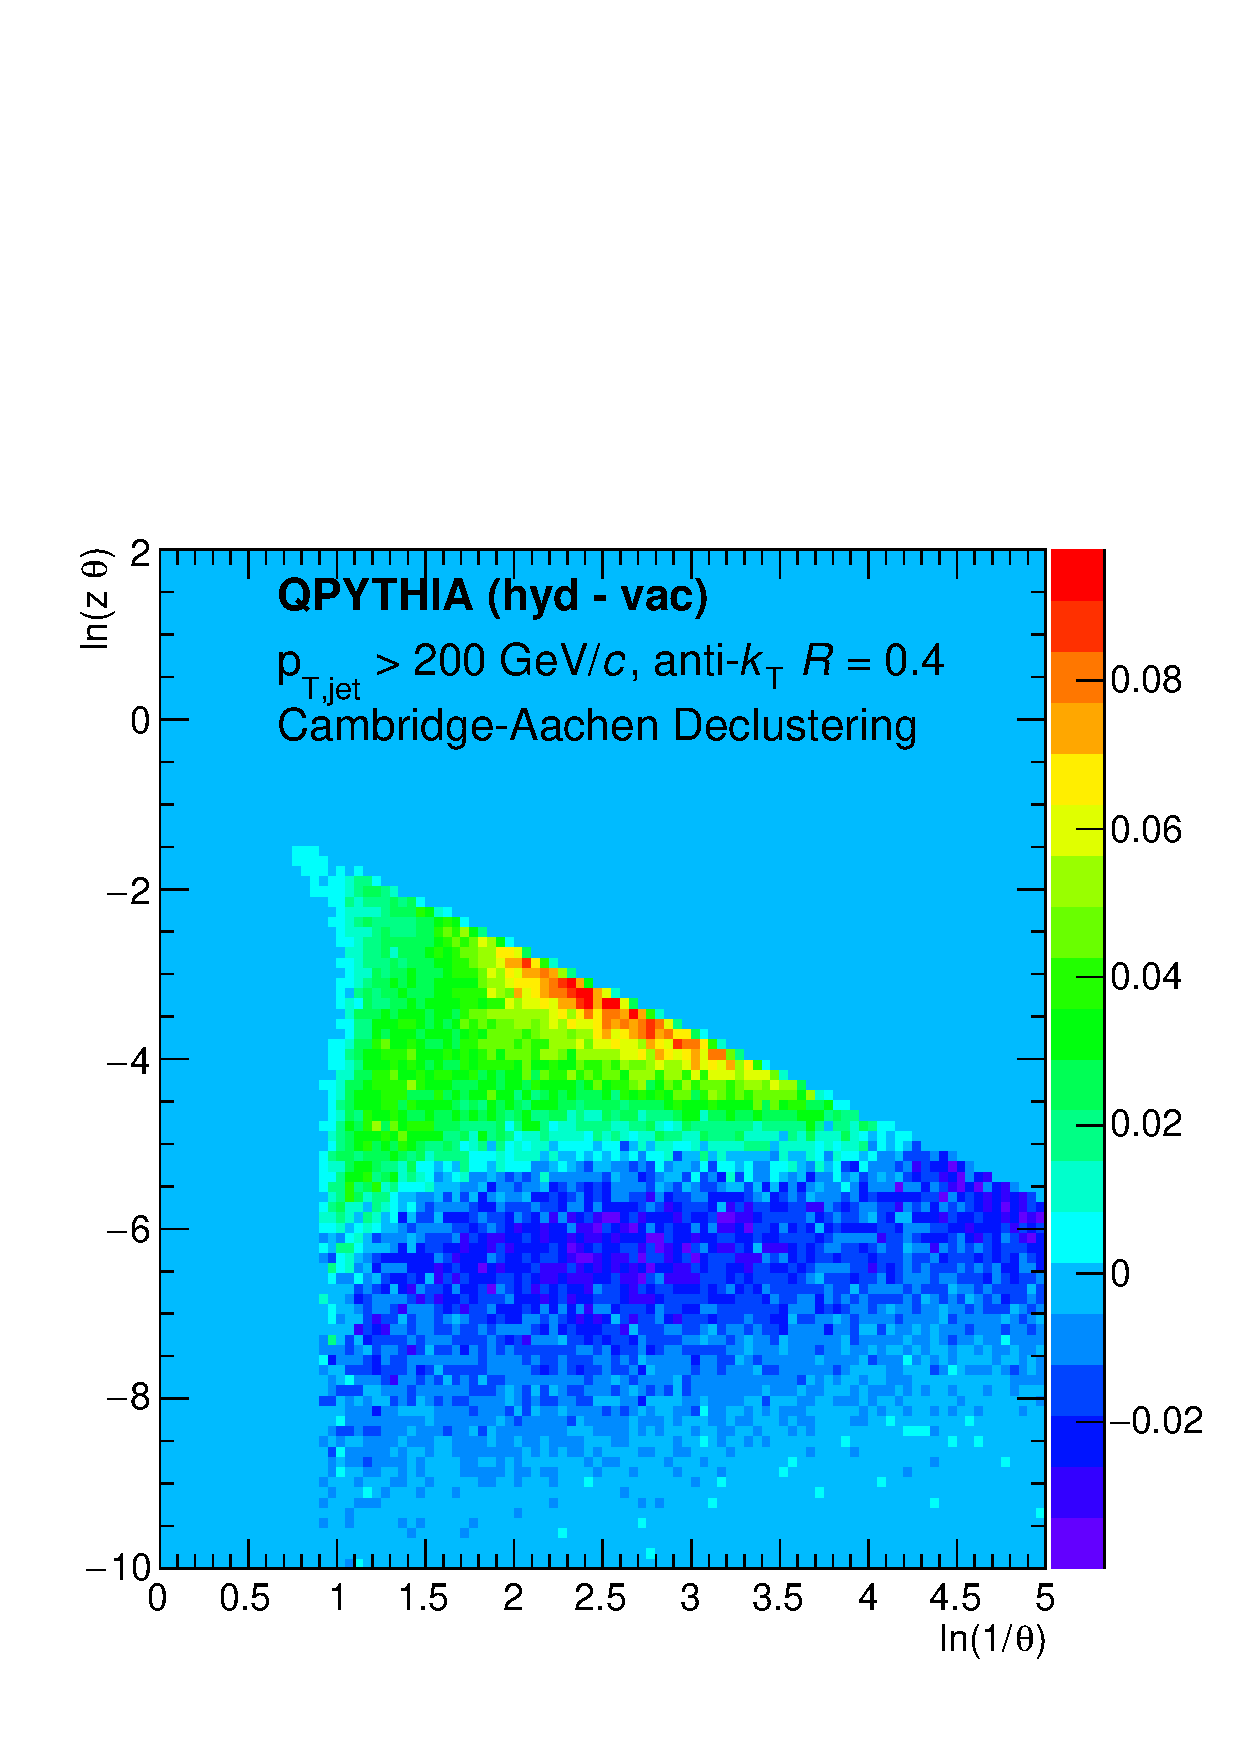
\includegraphics[width=0.3\textwidth]{figures/LundMC/QPythiaDiff200}
%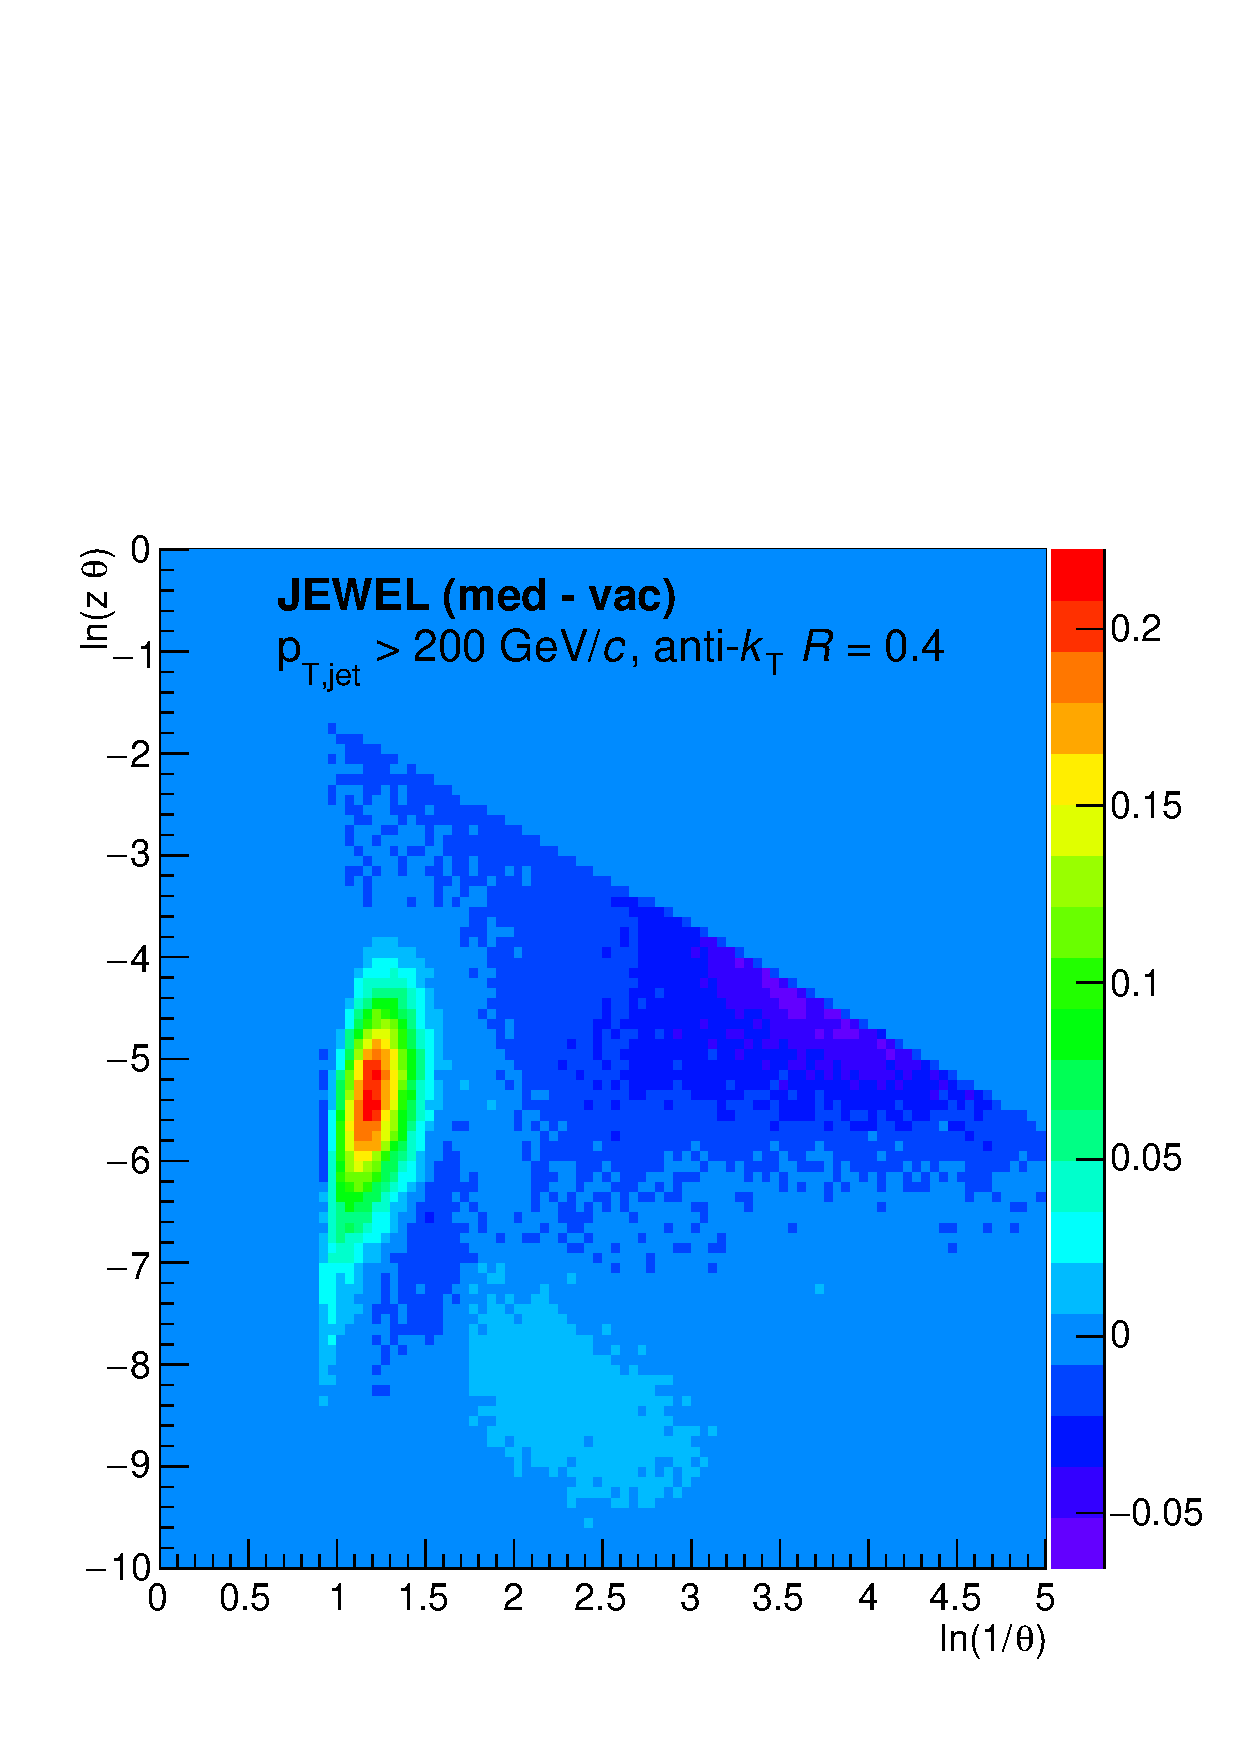
\includegraphics[width=0.3\textwidth]{figures/LundMC/JewelRecoilOffDiff}
%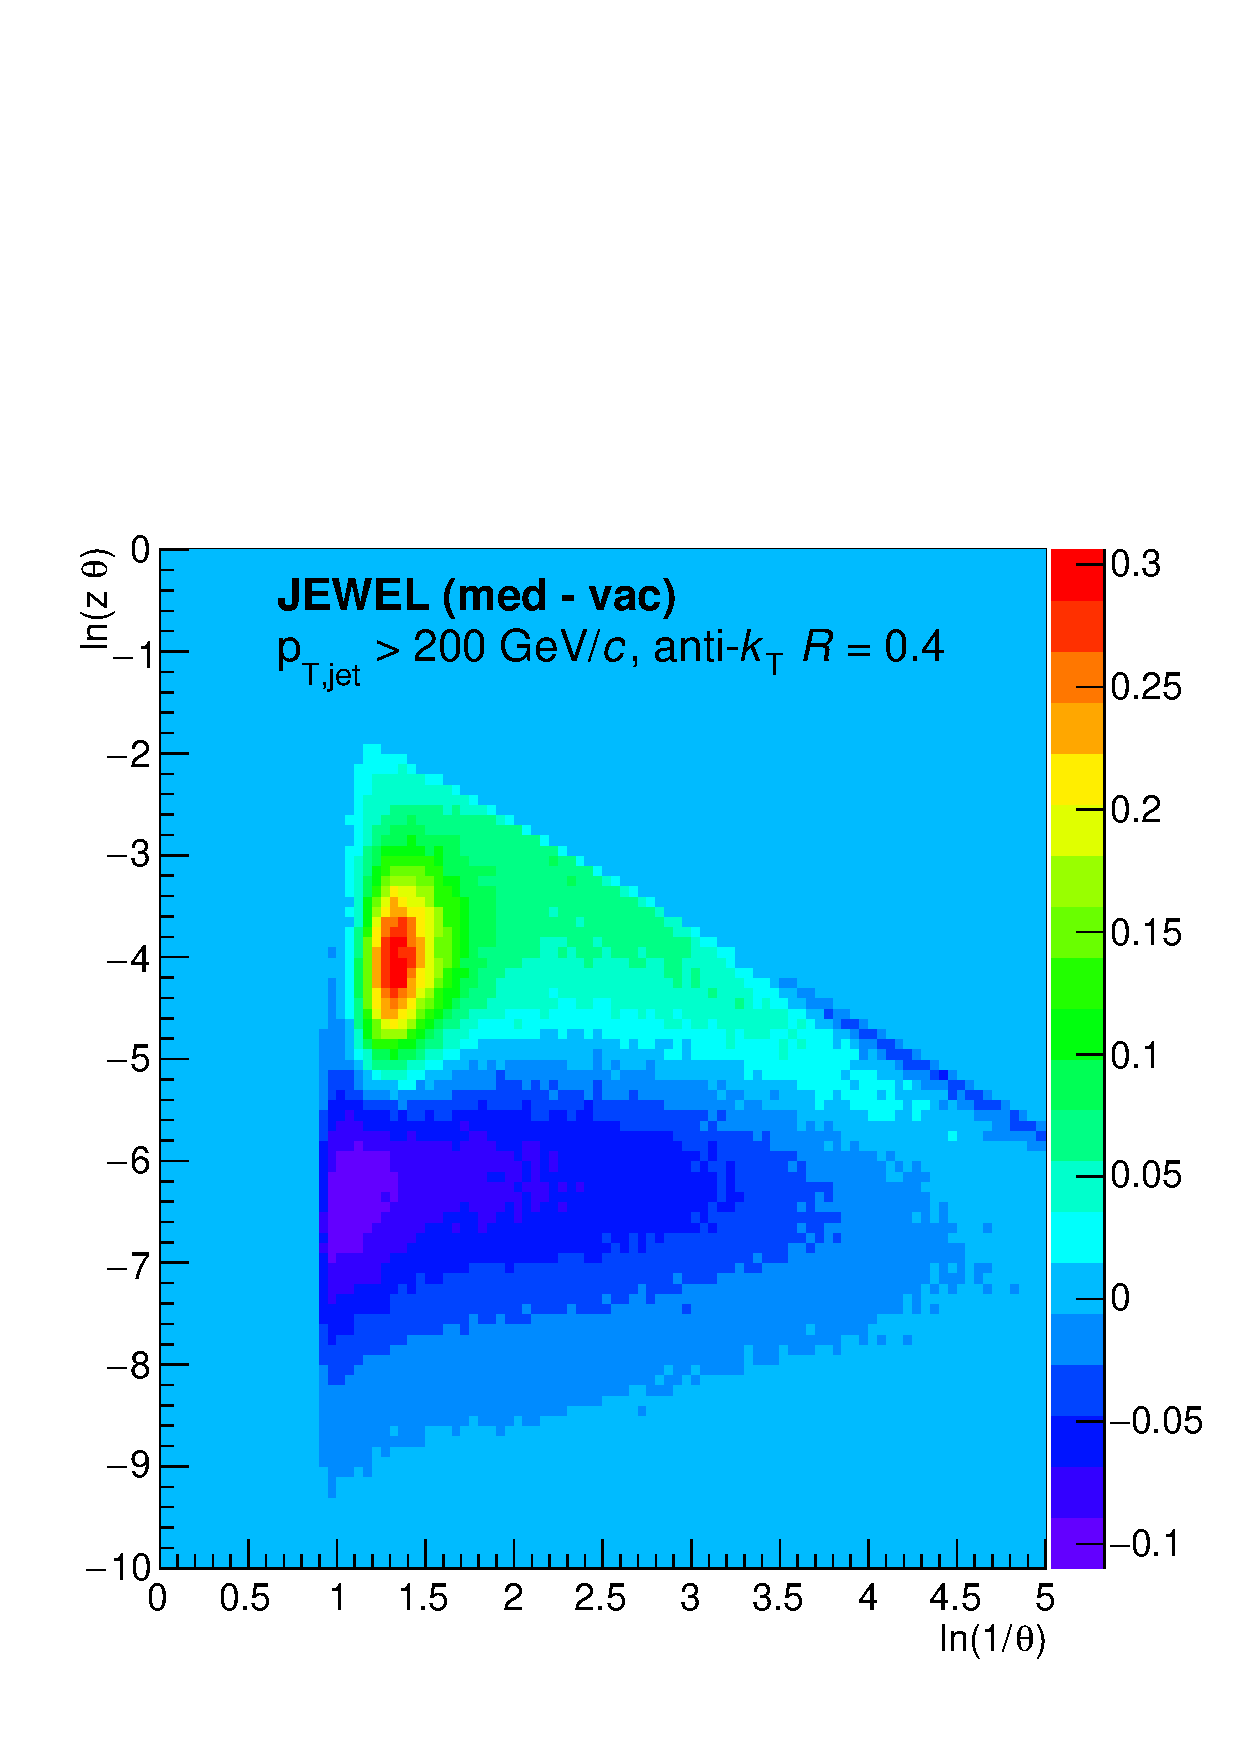
\includegraphics[width=0.3\textwidth]{figures/LundMC/JewelRecoilOnDiff}
%\caption{Lund diagram reconstructed from jets generated by QPYTHIA (left), JEWEL without recoils (middle) and JEWEL with recoils on.
%The lower panels correspond to the difference of the radiation pattern between with and without jet quenching.}
%\label{fig:PS2}
%\end{figure}
%%%%%%%%%%%%%%%%%%%%%%%%%%%%%%%%%%%%%%
%As a demonstration of the general ideas outlined above, we have filled the Lund diagram using PYTHIA 8, and two pQCD-based models for jet quenching, namely JEWEL (w/wo medium recoils) and QPYTHIA.  The variables $z\theta$ and $\theta$ have been reconstructed from subsequent branchings that were identified by reclustering the jet with a C/A algorithm.
%
%Fig.~\ref{fig:PS2Vac} shows the Lund diagram in vacuum and its characteristic horizontal bands due to the evolution of the coupling constant with the momentum scale are apparent. The excess of splittings at large angle seen in the left plot is caused by the PYTHIA underlying event, which is switched off in the right plot. 
%
%Fig.~\ref{fig:PS2}, upper plots, correspond to QPYTHIA, JEWEL w/o recoils and JEWEL w/ recoils respectively. The lower plots show the differences to the corresponding vacuum Lund diagrams.
%
%QPYTHIA exhibits an modest excess of large $k_{T}$ quanta relative to vacuum. In the model, the number of splittings is increased relative to vacuum leading to a significant intra-jet momentum broadening. 
%
%JEWEL generates additional medium-induced branchings that are not present in the vacuum reference. These are also allowed to branch further in the medium. In the difference plot we can clearly identify a modest excess of large-angle, semi-hard quanta in JEWEL. Interestingly, jet profiles calculated with JEWEL do not show an enhancement of momentum at large angles relative to vacuum \cite{KunnawalkamElayavalli:2017hxo}. A possible reason is that in the case of the jet profiles the angle is always measured relative to the jet axis while in our declustering approach the angles are always measured relative to the hardest parent or subjet, in which case the angular distribution can be broader. 
%Such excess becomes harder when the medium recoils are included. The nature and role of the recoils will be explained in the next subsection. 
%
%It is worth noting that the medium-induced signal populates different regions of phase space in the two jet quenching models. The choice of the grooming parameters in Eq. \ref{eq:groompar} is critical to enhance the sensitivity to the signal, as it will be discussed in the next section. 
%
%
%\subsubsection{Medium response}
%
%Jet quenching is expected to be accompanied by recoil effects. The jet induced medium response constitutes a correlated background that can contribute to the modifications of the measured jet substructure. Recoil effects are expected to contribute in the soft-large angle sector of the phase space, similarly to the uncorrelated underlying event, described in the next section. 
%
%JEWEL can be ran with and without recoiling partons entering the hadronisation. 
%The difference between the Lund diagrams for the two options is shown in Fig.~\ref{fig:PS2} lower right plot. 
%
%The impact of the recoils as modeled by JEWEL has being documented \cite{Milhano:2017nzm}\cite{KunnawalkamElayavalli:2017hxo}. Its contribution is needed to describe most of the jet shapes measured so far at the LHC. In particular, if the medium response can smear the subleading subjet momentum above the given grooming cut, the subjet momentum balance or $z_{g}$ can become more asymmetric relative to vacuum.   
%
%As a correlated background, the medium response cannot be experimentally subtracted
%to isolate purely radiative modifications to the jet shower. However, correlation of jet substructure observables might help to suppress it \cite{Milhano:2017nzm}. 
%\begin{figure}[th]
%\centering
%\includegraphics[width=0.33\textwidth]{figures/LundMC/JewelRecoilDiff.pdf}%
%\caption{Difference of the lund plots for JEWEL with recoils on and without}
%\label{fig:RecoilJewel}
%\end{figure}

%\clearpage
%\newpage
%%%%%%%%%%%%%%%%%%%%%%%%%%%%%%%%%%%%%
\subsection{Groomed substructure observables and sensitivity to jet quenching}
\label{sec:groomedobservables}
%%%%%%%%%%%%%%%%%%%%%%%%%%%%%%%%%%%%%

After identifying the first splitting that satisfies Eq.~(\ref{eq:groompar}), we have access to the full kinematics of that branching process. The groomed jet energy ($\pT = E$) is now defined as $p_{{\rm \tiny T} g} \equiv p_{\mathrm{T},1}+p_{\mathrm{T},2}$, where the subscripts now refer to the identified subjets. We can then define the groomed momentum fraction, $z_g = \min \left(p_{{\rm \tiny T},1},p_{{\rm \tiny T},2}\right)/p_{{\rm \tiny T}g}$ and the angle $\Delta R_{12}$ between the subjets. In our numerical studies, we will focus on these two quantities but also introduce the groomed mass to energy ratio $M_g/\pT$, where $M_g$ is defined as in Eq.~(\ref{eq:DipoleMass}) with all relevant quantities being groomed. These observables shed light on how the branchings occur in course of the parton shower and are sensitive to medium effects as long as the branching originates from inside the medium, roughly corresponding to $ t_{{\rm f}g}\equiv 2 p_{{\rm \tiny T}g}/M_g^2 < L$, see discussion above. For the chosen medium parameters, the samples analyzed with settings SD1 and SD2 will contain an admixture of in-medium and out-of-medium splittings, see \autoref{fig:TheorySD}, while SD3 picks exclusively out hard splittings originating from inside the medium. 

As in the previous section, the jet quenching Monte Carlo event generators we use in our study are QPYTHIA and JEWEL (with recoil effects turned on and off) and are shown in \autoref{fig:SDGenZG}, \ref{fig:SDGenDR12} and \ref{fig:SDGenMg}. Jets were reconstructed using anti-$k_{\rm \tiny T}=0.4$ and for $\pT > 130$ GeV/c. 
The results in this section are obtained at generator level, without embedding. In particular, we have not introduced any detector resolution effects, such as a minimal angular cut-off $\Delta R_{\rm min}$.
Note, that the distributions are normalized by the total number of anti-$k_{\text{T}}$ (ungroomed) jets. The distributions are therefore not self-normalized and contain information how grooming affects the overall suppression of the jet yield. 

%%%%%%%%%%%%%%%%%%%%%%%%%%%%%%%%%%%%%
\begin{figure}[t]
\centering
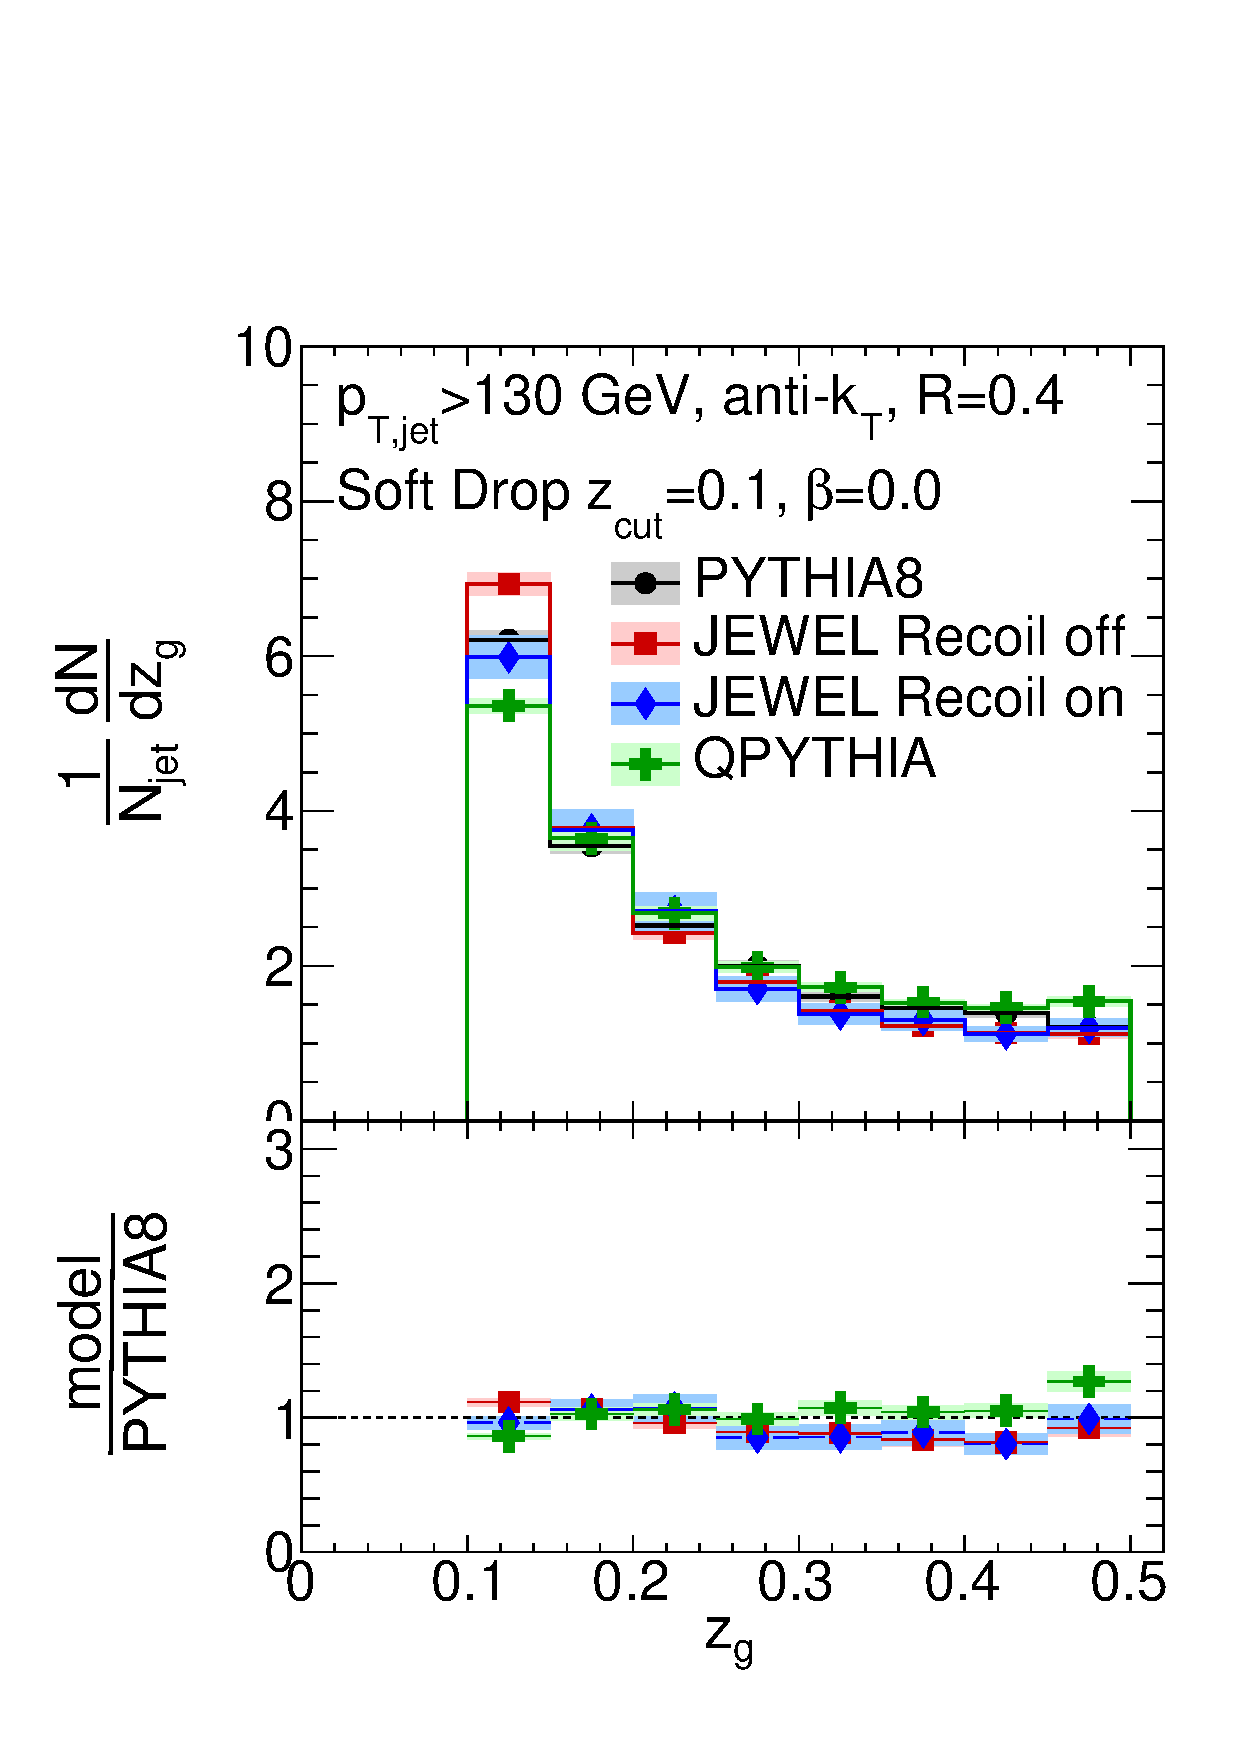
\includegraphics[width=0.33\textwidth]{figures/SDGen/ZgCompModelsBeta00Z01.pdf}%
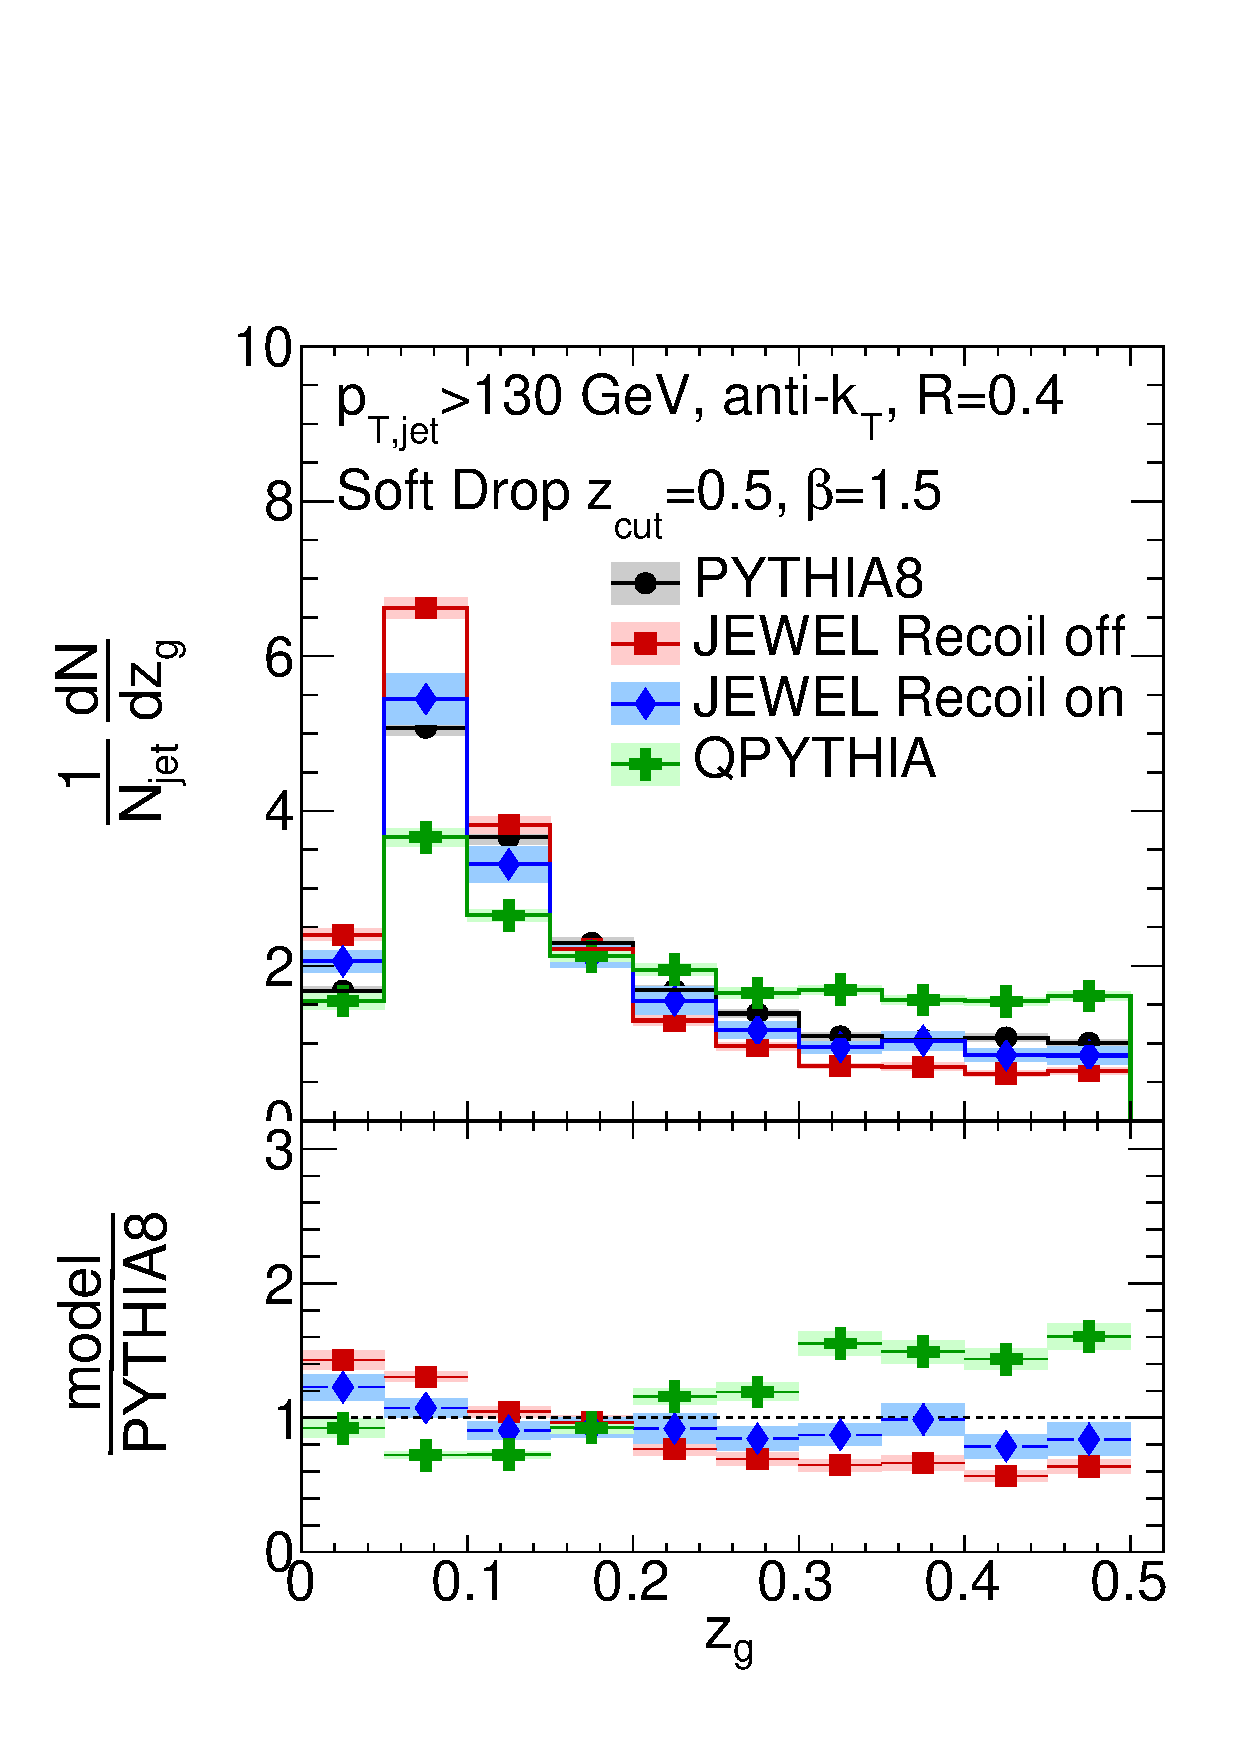
\includegraphics[width=0.33\textwidth]{figures/SDGen/ZgCompModelsBeta15Z05.pdf}%
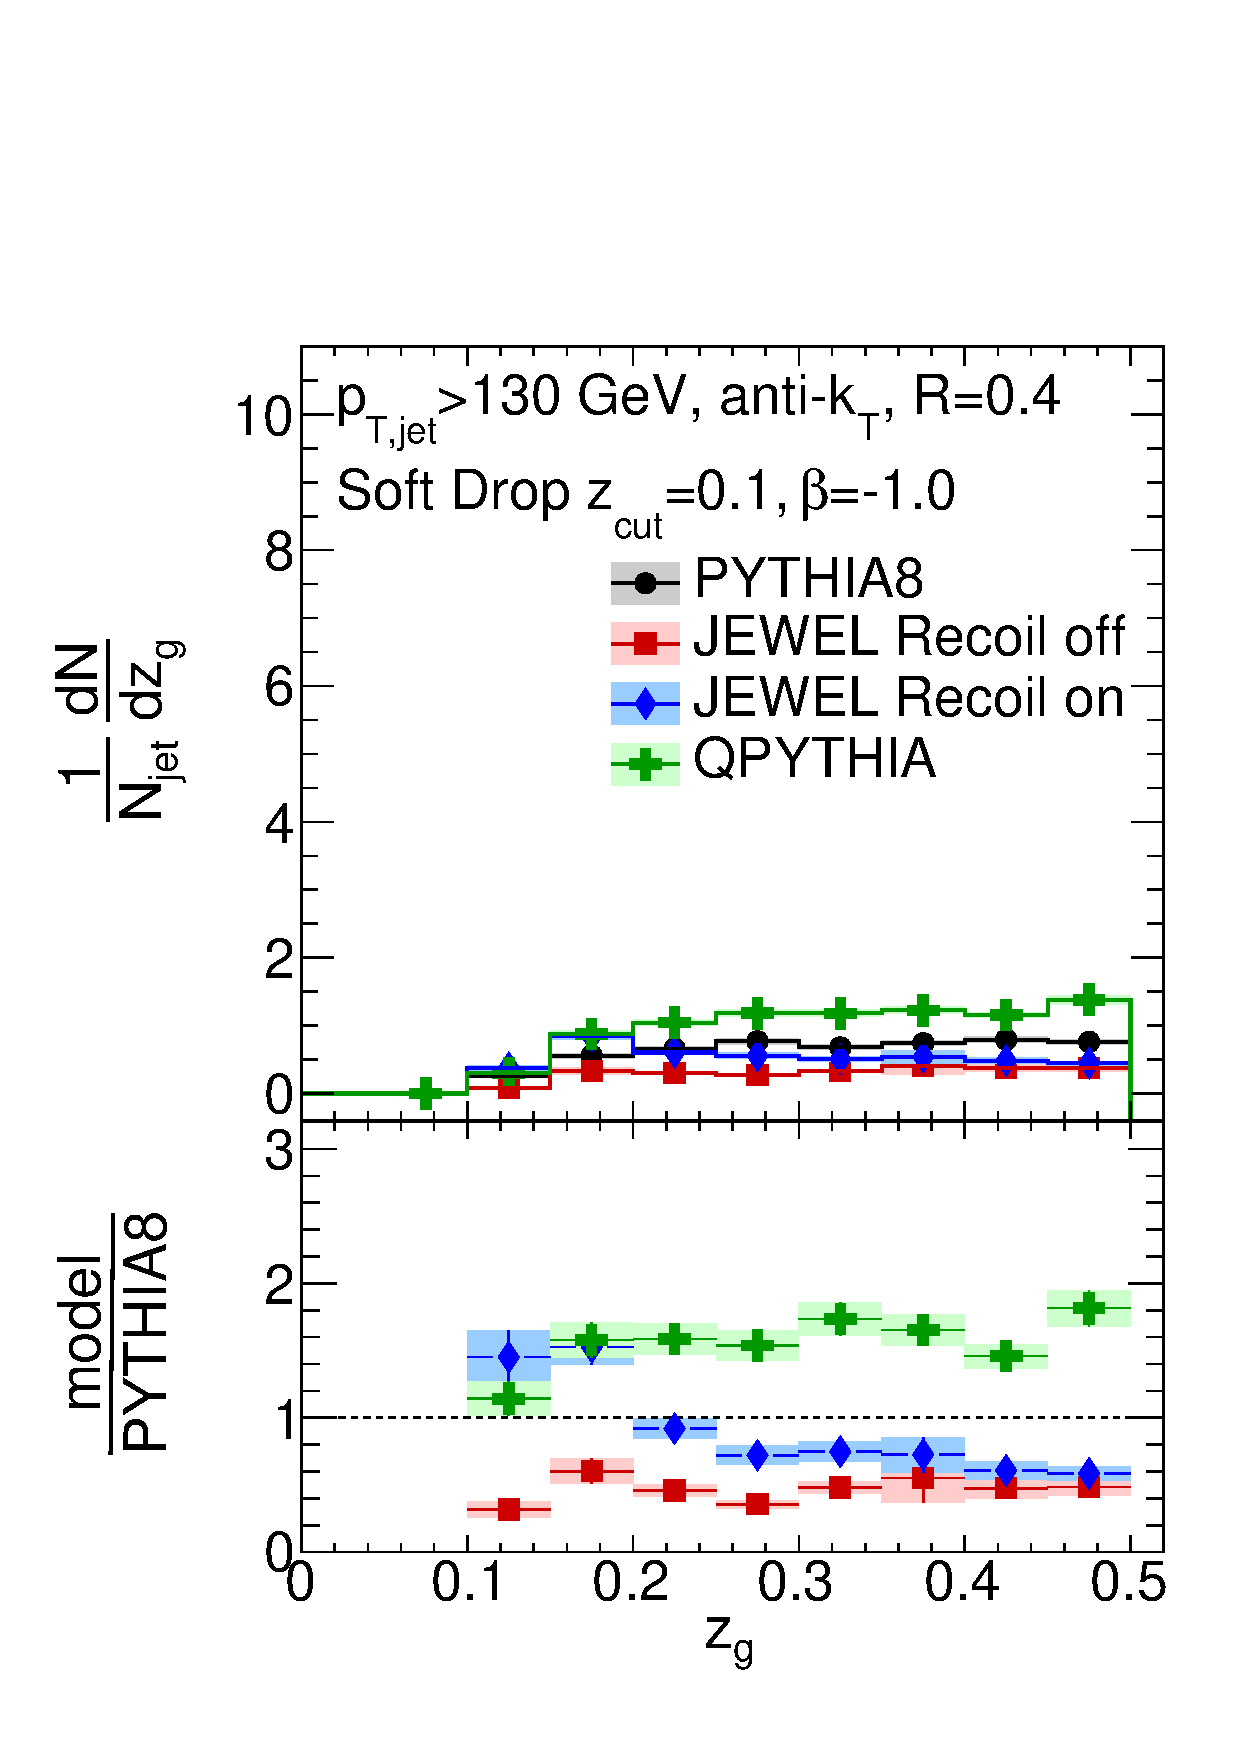
\includegraphics[width=0.33\textwidth]{figures/SDGen/ZgCompModelsBetam1Z01.pdf}%
\caption{Groomed shared momentum fraction, $z_{\mathrm{g}}$, for three different grooming settings in simulations with and without jet quenching. The uppers panels show the $z_{\mathrm{g}}$ distribution normalized by the total number of ungroomed jets while the lower panels show the ratio of JEWEL and QPYTHIA with respect to PYTHIA8.}
\label{fig:SDGenZG}
\end{figure}
%%%%%%%%%%%%%%%%%%%%%%%%%%%%%%%%%%%%%
Figure~\ref{fig:SDGenZG} shows the momentum fraction $z_g$ distribution for different event generators. The vacuum baseline is represented by the PYTHIA8 data points and compared to results from the QPYTHIA and JEWEL jet quenching event generators.
In this figure, the perhaps most striking feature is the generally opposite trend of the two models. This can also be traced back to the discussion around \autoref{fig:PS2}. The modified parton shower in QPYTHIA makes the jets broader with respect to jets in vacuum and therefore many more jets survive the grooming. JEWEL however collimates the jets and therefore less jets are surviving the grooming with this setting.

We also note, that while for $\beta \geq 0$, see \autoref{fig:SDGenZG} (left and center), the number of jets for the different generators remains roughly constant while for the negative grooming setting $\beta < 0$, \autoref{fig:SDGenZG} (right), a large deviation from unity can be observed. Interestingly, QPYTHIA subjets are strongly enhanced in this regime while JEWEL ``Recoils off'' subjets are strongly suppressed, both by a factor $\sim1.5-2$. Note also that the magnitude of effects are the biggest for the most aggressive setting that naively corresponds to early in-medium splittings.

Comparing the JEWEL results with and without recoil demonstrates that, for the chosen analysis settings, this observable is not very sensitive to recoil effects except for the small-$z_g$ region.
%The tightest setting $\beta < 0$ is notably very resilient.
In order to compare to the data presented in \cite{Sirunyan:2017bsd} for the $\beta=0$ setting, see also \cite{Milhano:2017nzm} for a study using JEWEL, where a significant deviation from vacuum baseline was observed, we again point out that no minimal angular cut-off was employed in our studies. Such a cut-off suppresses collinear vacuum radiation and, hence, amplifies the effects related to the medium.

%%%%%%%%%%%%%%%%%%%%%%%%%%%%%%%%%%%%%
\begin{figure}[th!]
\centering
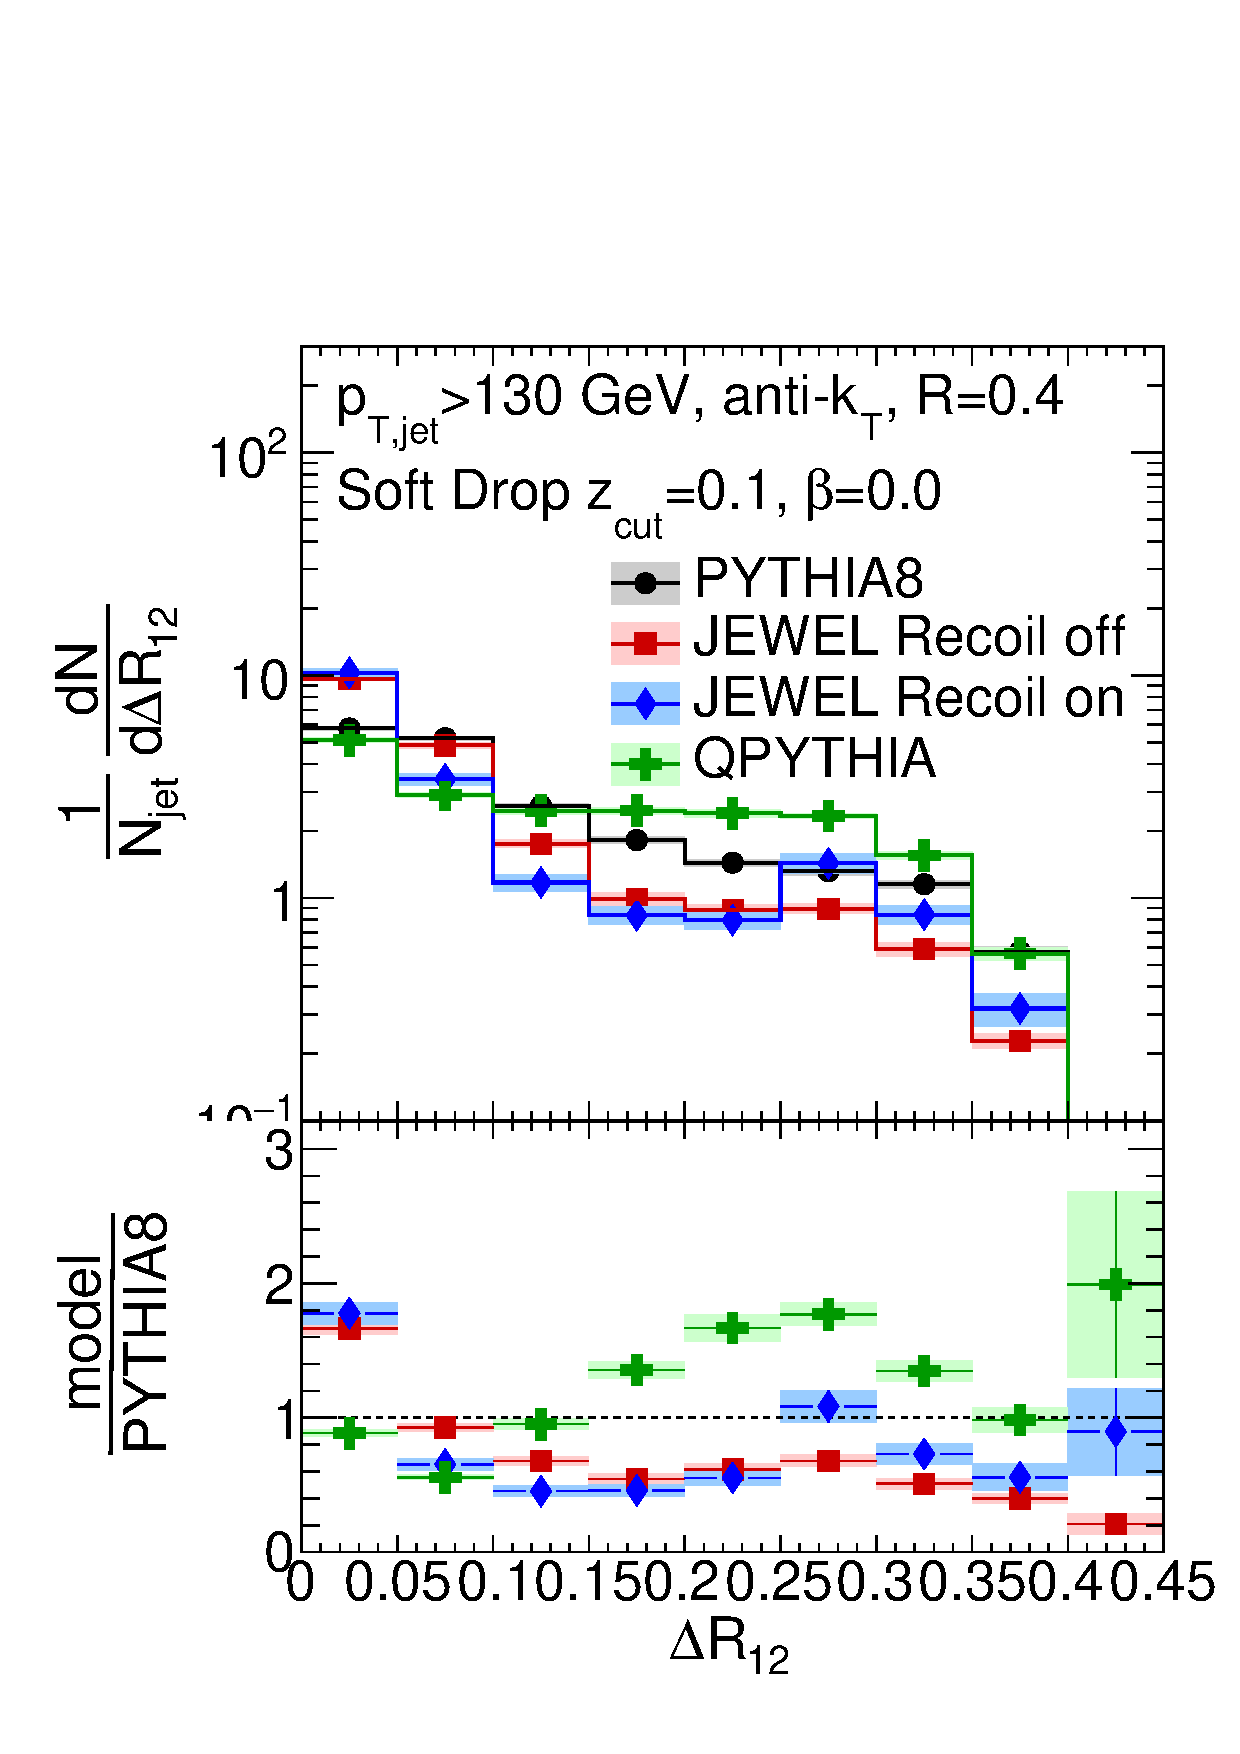
\includegraphics[width=0.33\textwidth]{figures/SDGen/DR12CompModelsBeta00Z01.pdf}%
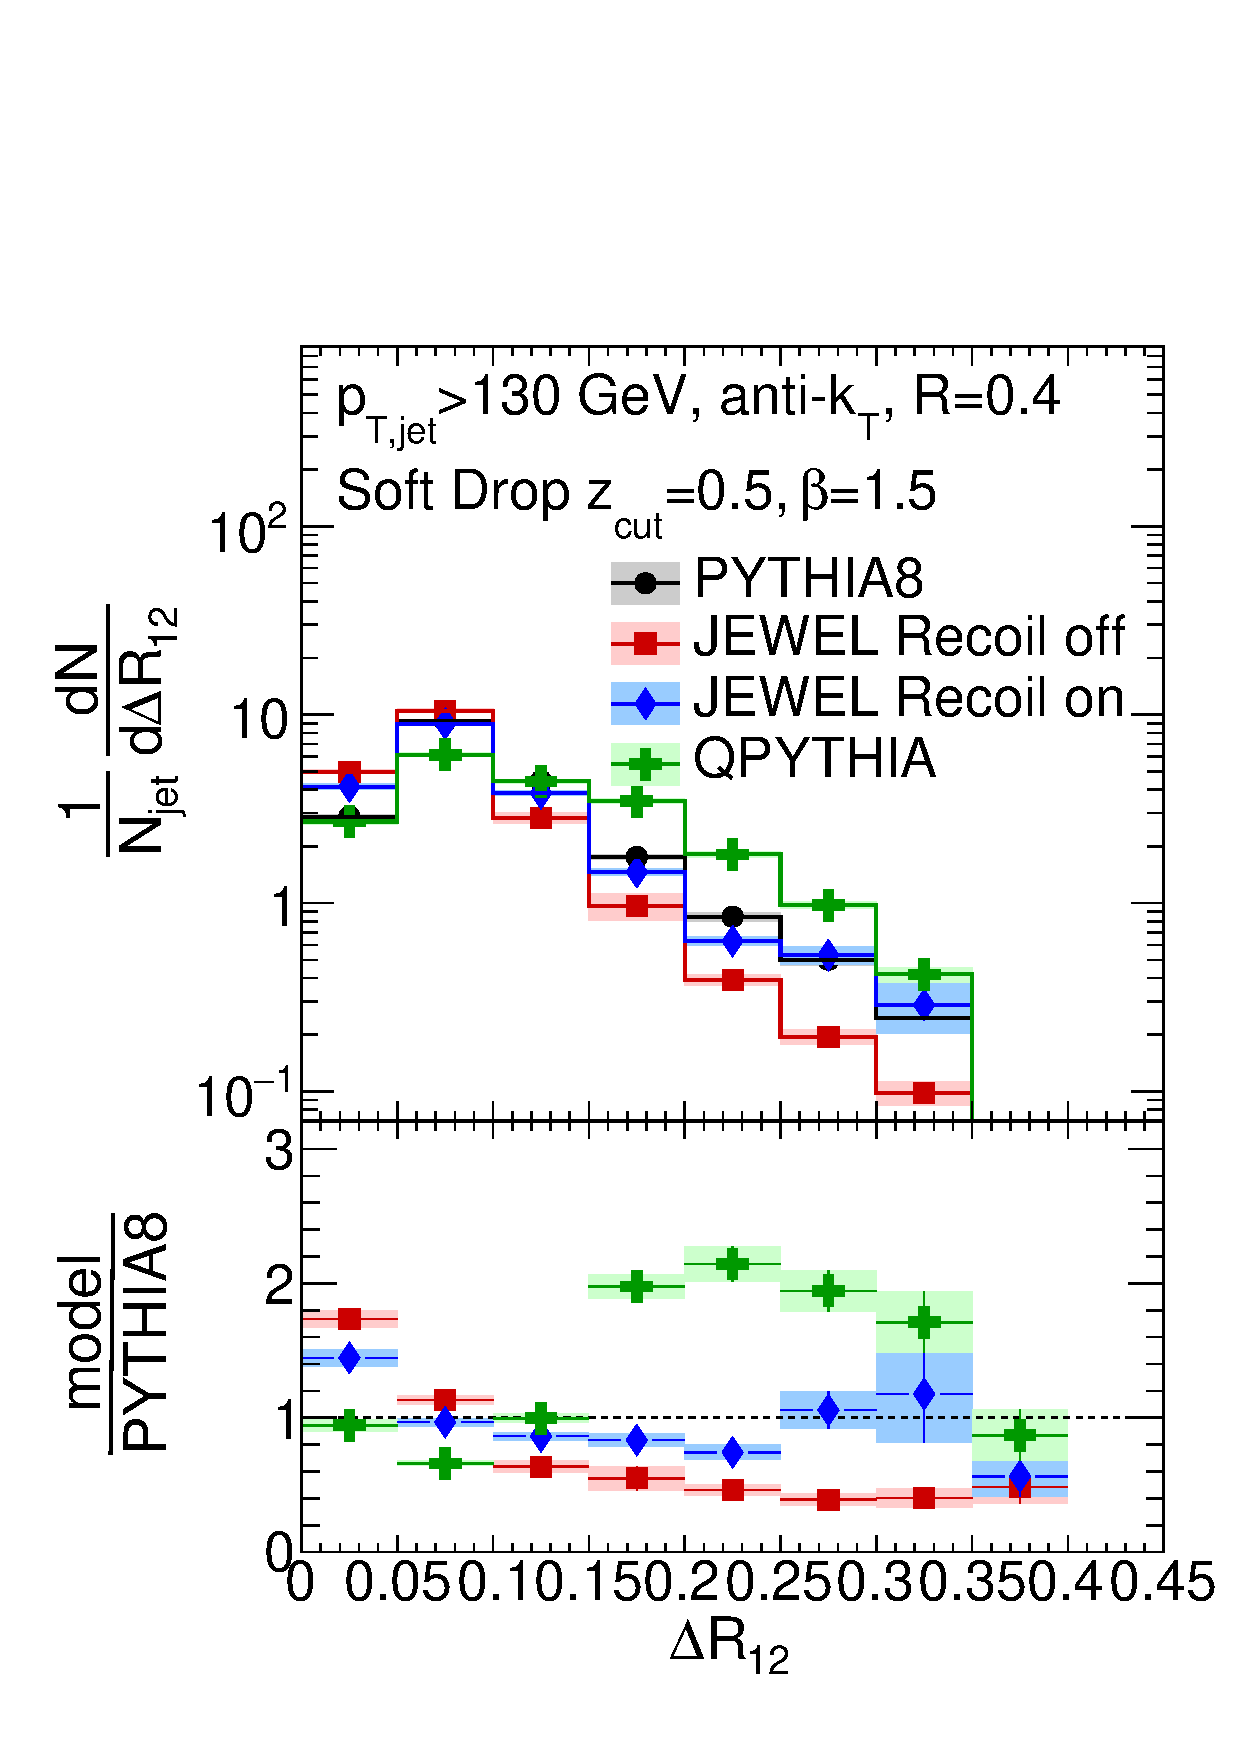
\includegraphics[width=0.33\textwidth]{figures/SDGen/DR12CompModelsBeta15Z05.pdf}%
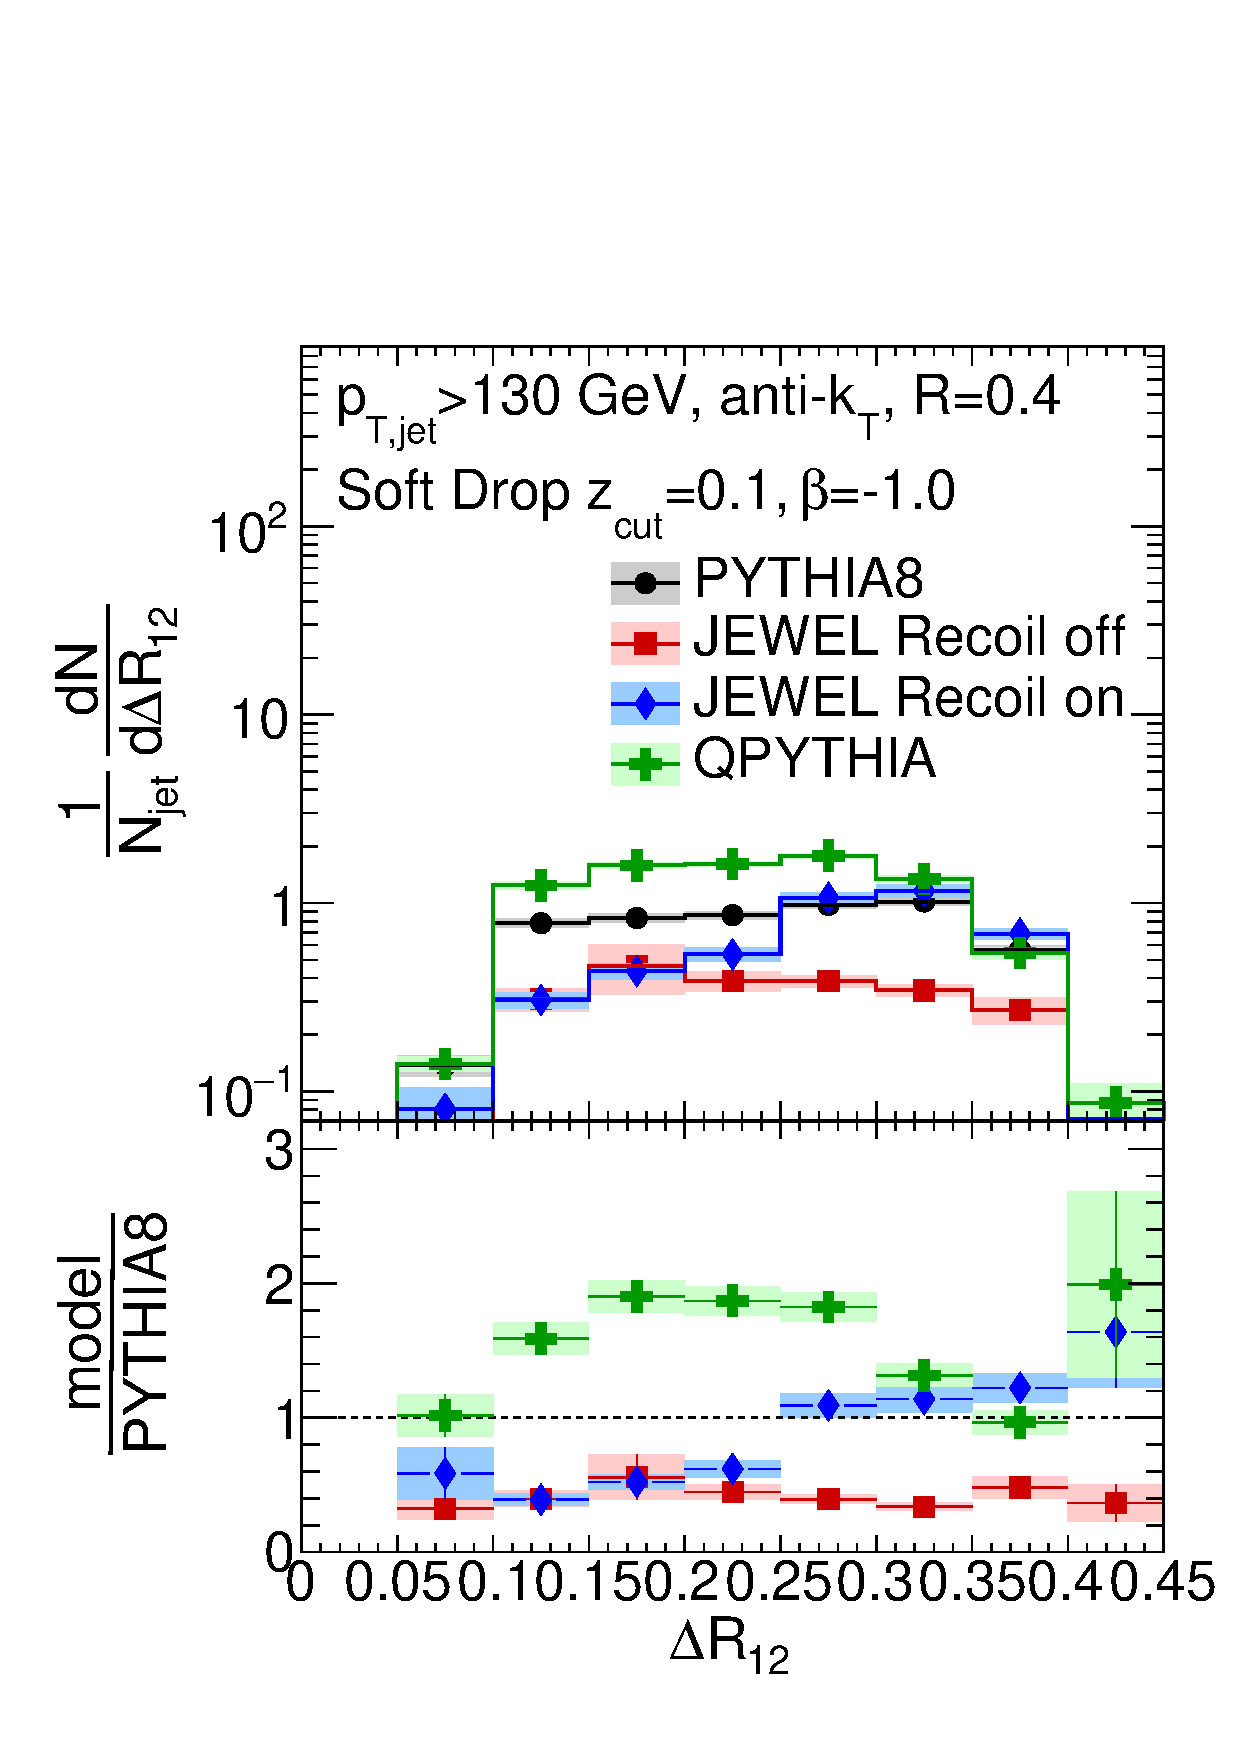
\includegraphics[width=0.33\textwidth]{figures/SDGen/DR12CompModelsBetam1Z01.pdf}%
\caption{Distance between the two groomed subjets, $\Delta R_{12}$, for three different grooming settings in simulations with and without jet quenching. The uppers panels show the $\Delta R_{\mathrm{12}}$ distribution normalized by the total number of ungroomed jets while the lower panels show the ratio of JEWEL and QPYTHIA with respect to PYTHIA8.}
\label{fig:SDGenDR12}
\end{figure}
%%%%%%%%%%%%%%%%%%%%%%%%%%%%%%%%%%%%%
Next we turn to studying the angular separation $\Delta R_{12}$ distribution of the groomed subjets. In the context of jet quenching, one particularly interesting question is to gauge whether substructures are quenched relative to their angular separation. The angular distance between the groomed sub-jets is plotted in \autoref{fig:SDGenDR12} for the three grooming settings. Once again, we see big differences between the MC models; JEWEL ``Recoils off'' being very collimated and QPYTHIA very broad. 
The JEWEL ``Recoils on'' setting interpolates between the two extremes and, most strikingly, exhibits an enhancement at intermediate angles, consistent with earlier studies of jet shape and fragmentation function \cite{KunnawalkamElayavalli:2017hxo}.

Once again, it is interesting to point out that the modifications are arguably the strongest for the most conservative SD setting, see \autoref{fig:SDGenDR12} (right). In particular, the JEWEL ``Recoils off'' samples are consistently suppressed for all angles. This could point to the importance of energy-loss that is not very sensitive to angle in JEWEL. The enhancement seen at small $\Delta R_{12}$ for $\beta \geq 0$, see \autoref{fig:SDGenDR12} (left, center), could also indicate a similar mechanism related to migration of narrow jets from higher $\pT$.
%The effect in JEWEL primarily shows up at large angels for all explored grooming settings. 
%In the JEWEL samples with $\beta \geq 0$ one observes larger sensitivity to recoil effects than for $\beta < 0$, which is remarkably flat for a wide range of angles.

%We note, in particular, a strong resilience to recoil effects in the JEWEL samples for all SD settings. Due to the suppression of large-angle jet structures in JEWEL (collimation), the small $M_g$ region is significantly enhanced compared to the vacuum baseline. 

%{\color{red} An interesting feature is perhaps that JEWEL is modified for small $M_g$ which technically implies that the splitting takes place outside of the medium. This is of course related to the enhancement seen at very small $\Delta R_{12}$. What is the reason for this modification? QPYTHIA is not modified there.}
%%%%%%%%%%%%%%%%%%%%%%%%%%%%%%%%%%%%%
\begin{figure}[th]
\centering
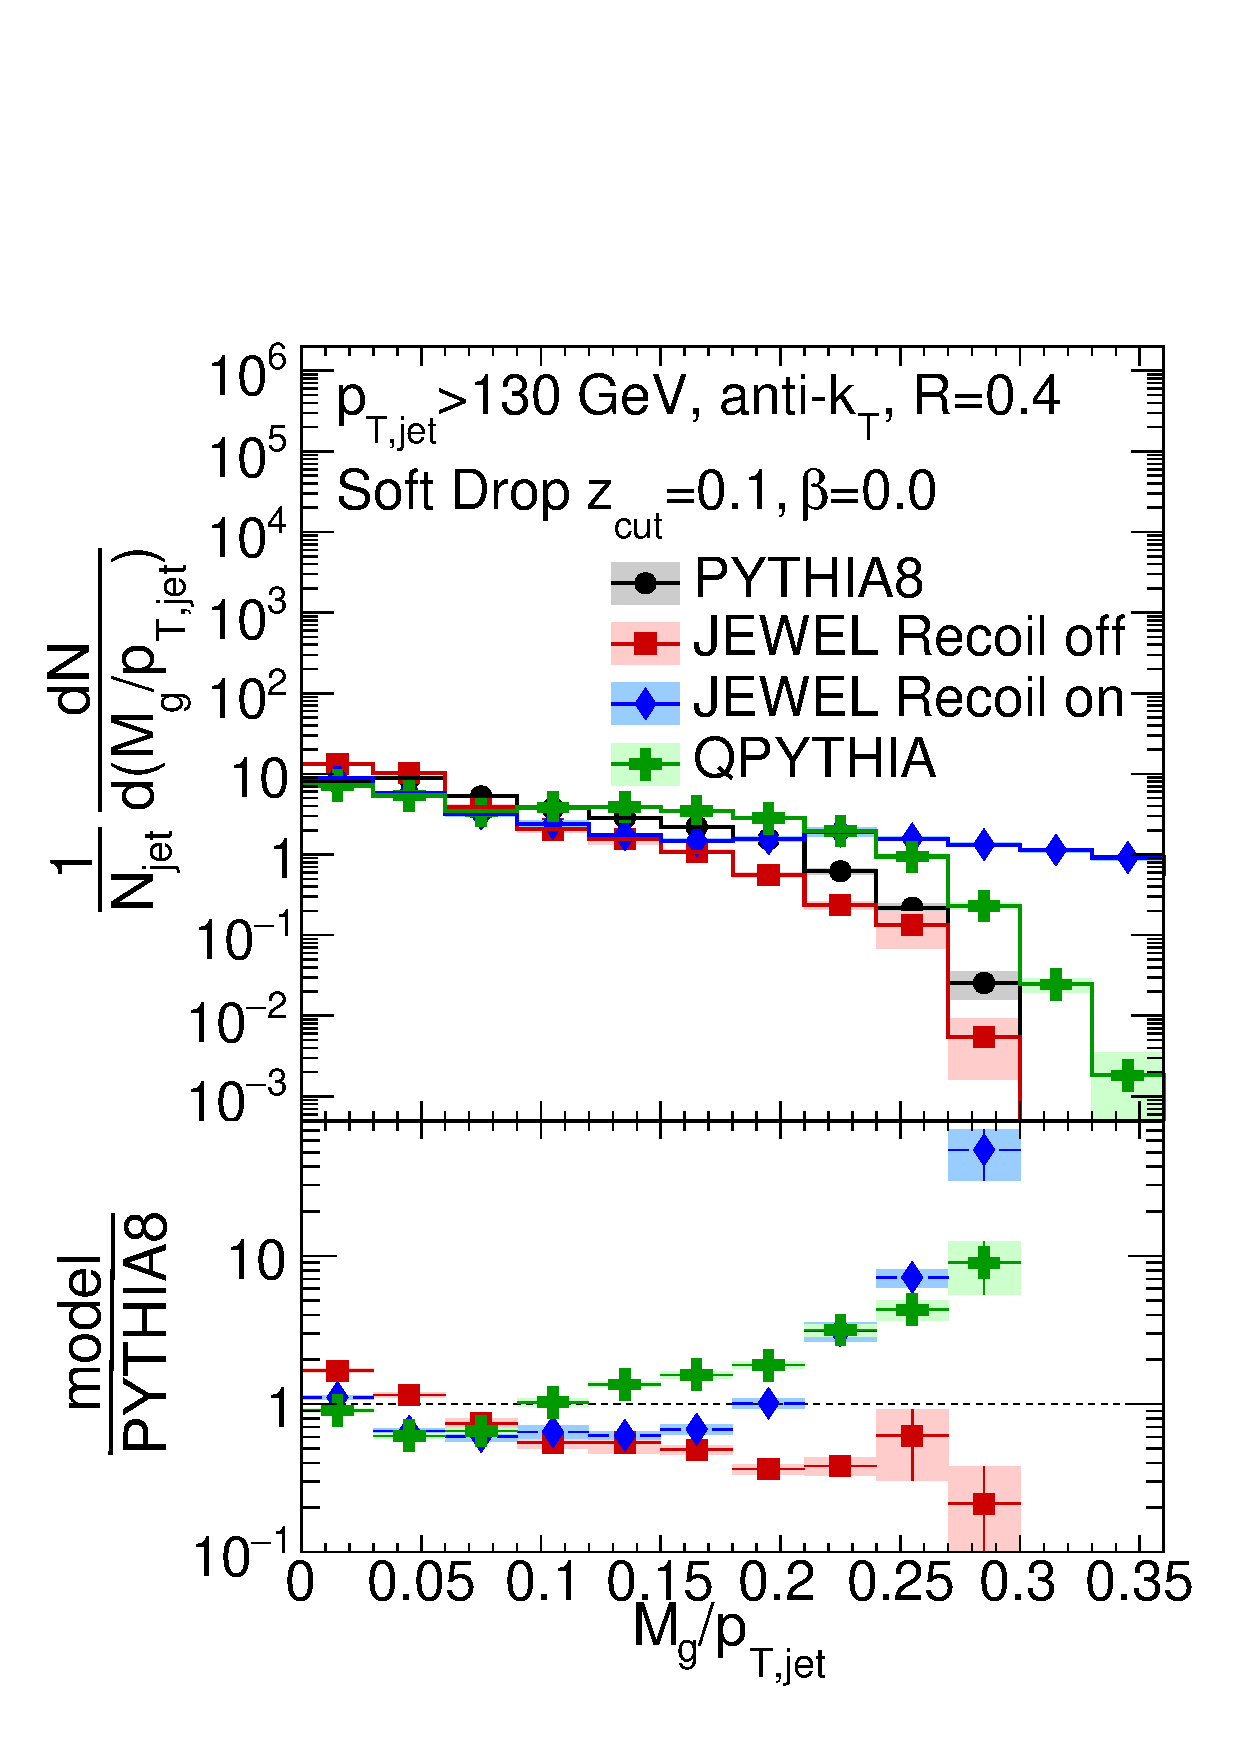
\includegraphics[width=0.33\textwidth]{figures/SDGen/MgOverPtgCompModelsBeta00Z01.pdf}%
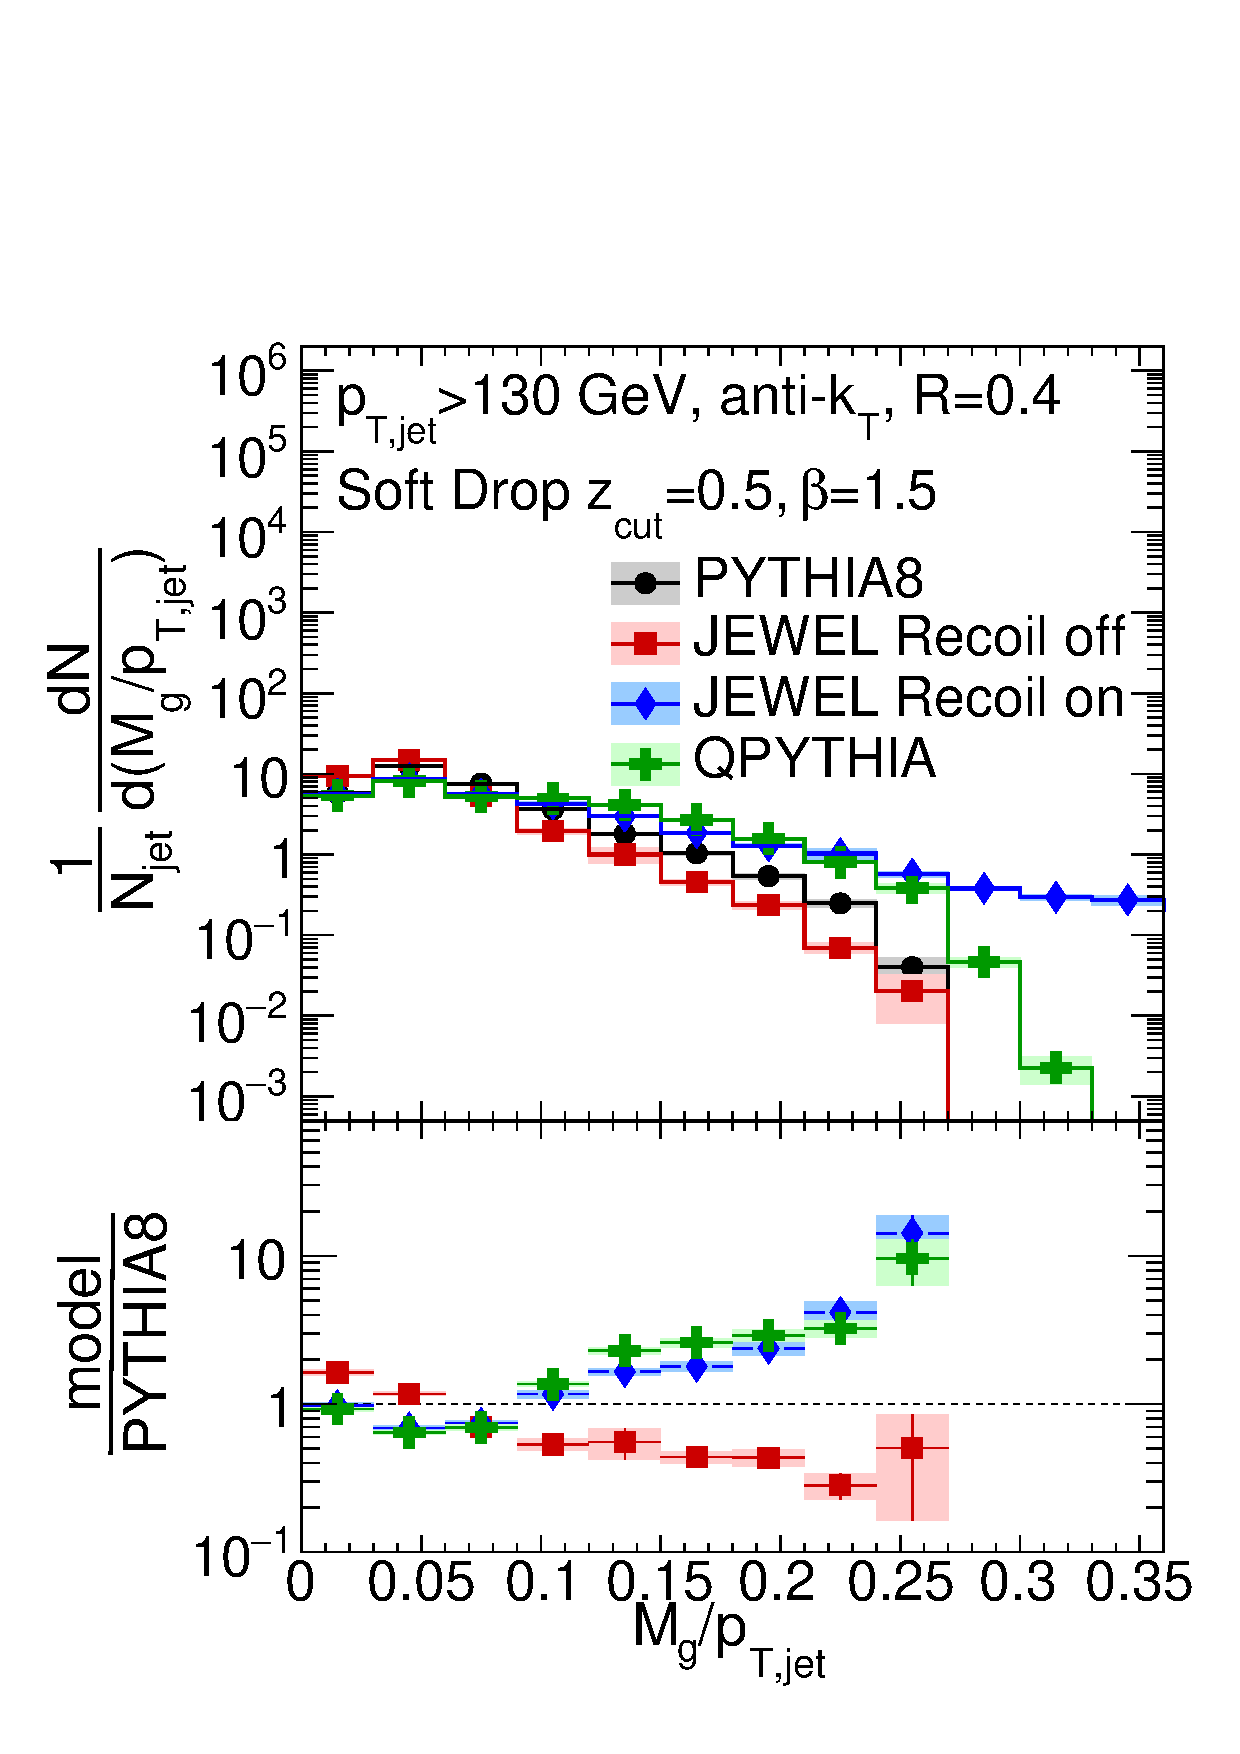
\includegraphics[width=0.33\textwidth]{figures/SDGen/MgOverPtgCompModelsBeta15Z05.pdf}%
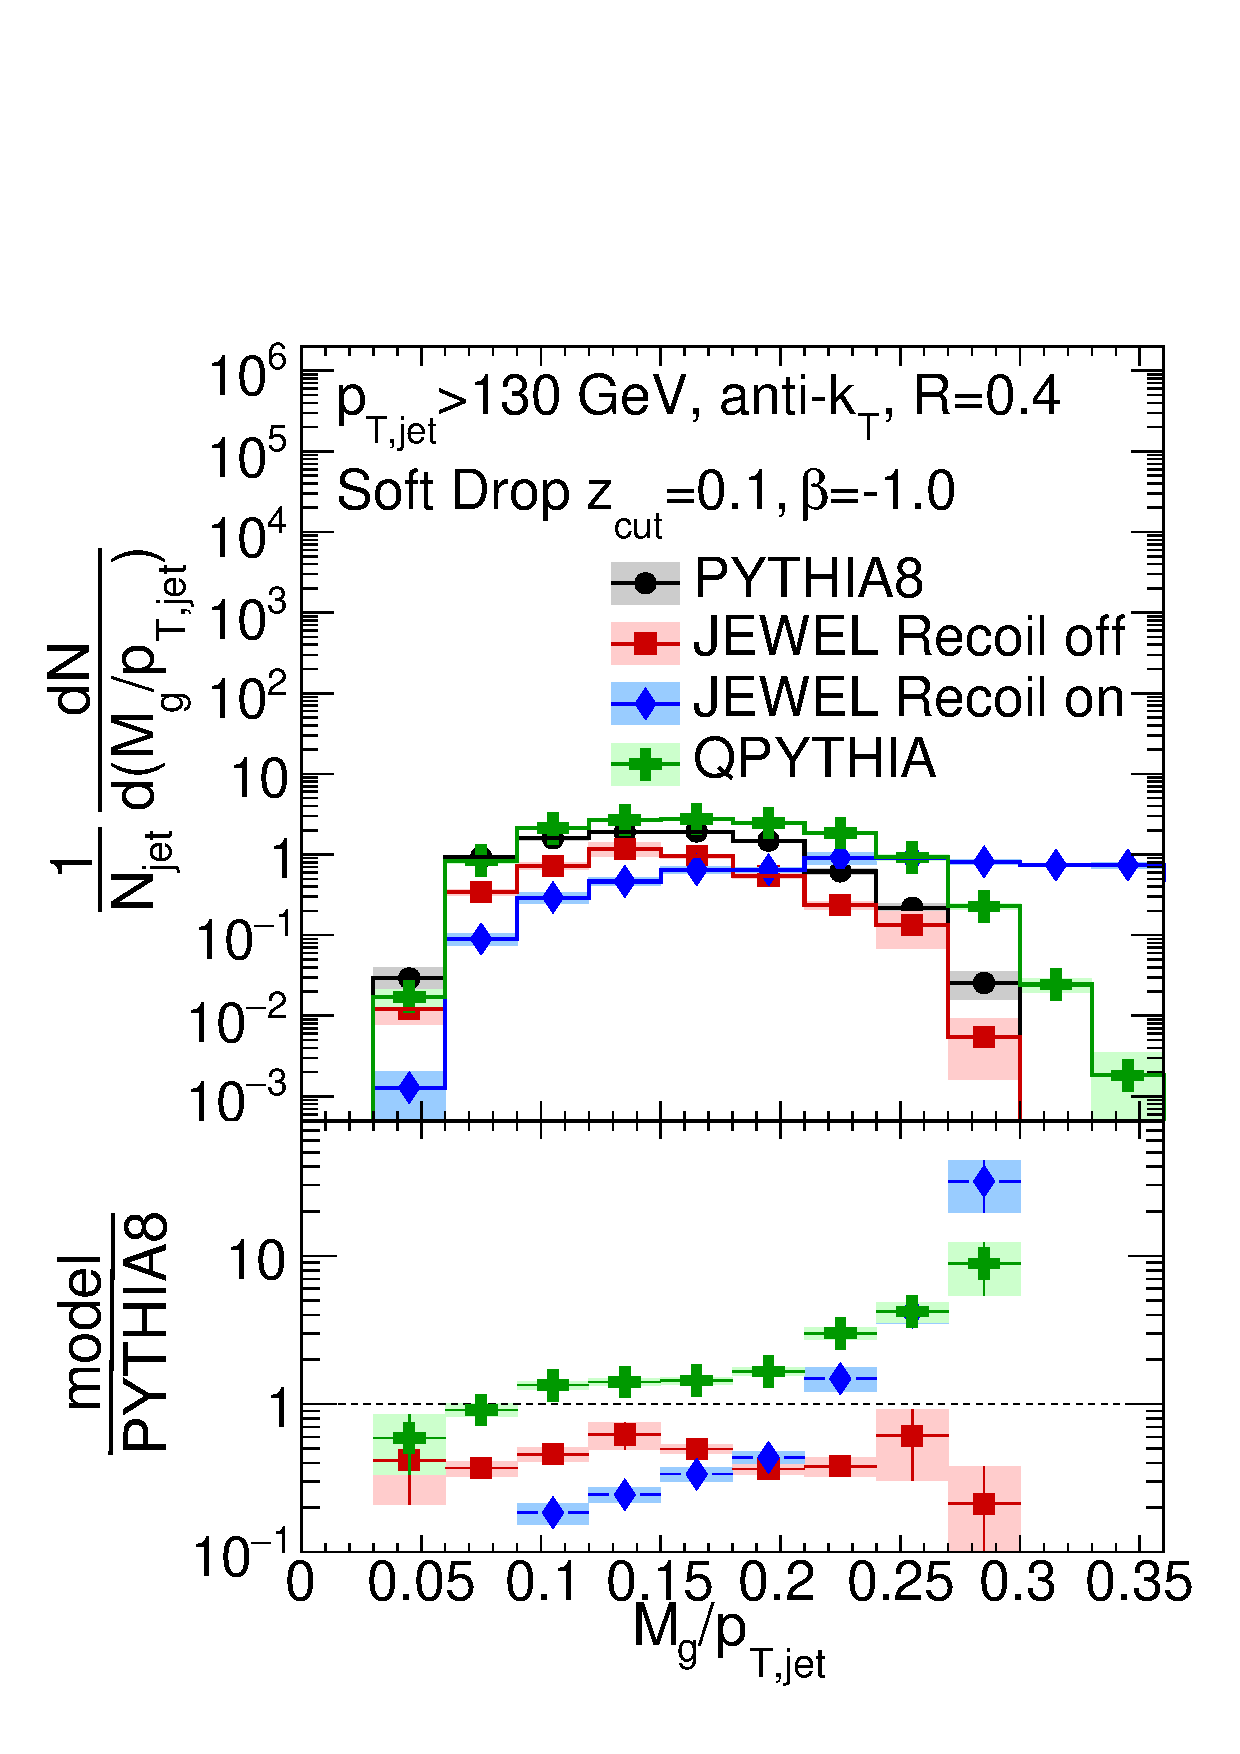
\includegraphics[width=0.33\textwidth]{figures/SDGen/MgOverPtgCompModelsBetam1Z01.pdf}%
\caption{Groomed jet mass, $M_{\mathrm{g}}/p_{\mathrm{T,jet}}$, for three different grooming settings in simulations with and without jet quenching. The uppers panels show the $M_{\mathrm{g}}/p_{\mathrm{T,jet}}$ distribution normalized by the total number of ungroomed jets while the lower panels show the ratio of JEWEL and QPYTHIA with respect to PYTHIA8.
%\kmt{Yi: gen-level makes sense, with embedding mass gets enhanced.}
}
\label{fig:SDGenMg}
\end{figure}
%%%%%%%%%%%%%%%%%%%%%%%%%%%%%%%%%%%%%
Finally, we study the groomed jet mass normalized by the transverse momentum, $M_{\mathrm{g}}/p_{\mathrm{T,jet}}$, in \autoref{fig:SDGenMg}. 
This observable combines several of the features already seen before and seems particularly constraining of large-mass jet substructures. In this case, the QPYTHIA and JEWEL ``Recoils on'' samples give rise to similar distributions with a strong enhancement at large $M_g/\pT$. The enhancement is the largest for the latter model. In contrast, JEWEL ``Recoils off'' is more resilient and exhibits a mild suppression with respect to vacuum results at high-masses. This could again be interpreted as an effect of energy-loss.
During the preparation of the workshop report results on the groomed mass in heavy-ion collisions at the LHC was released by the CMS collaboration \cite{Sirunyan:2018gct}. 

To summarize, these generator level studies of the kinematics of the subjet samples obtained using Soft Drop illustrates the wide range of sensitivity to different kinematical regimes, and therefore different effects. Further studies, including embedding and involving more medium models, are planned for the future and could help further constrain large classes of medium effects.

%%\clearpage
%%\newpage
%%%%%%%%%%%%%%%%%%%%%%%%%%%%%%%%%%%%%%%%%%
%\subsection{Sensitivity to reclustering algorithm} {\color{green} Leticia, Harry}
%\label{sec:reclusteringalgo}
%%%%%%%%%%%%%%%%%%%%%%%%%%%%%%%%%%%%%%%%%%
%The strategy of the clustering algorithm manifests itself in the declustering and grooming. CA algorithm combines the closest particles first. As a consequence, the first declustering steps will encounter soft splittings at large angle. In the case of k$_{T}$ algorithm, the softest particles are clustered first. As a consequence, the first declustering steps will encounter hard splittings. Anti-k$_{T}$ clusters hard particles first, thus splittings at the first declustering steps will be generally soft. Such ordering is reflected in the Lund plots of \autoref{fig:AlgoDependence}.
%\begin{figure}[th]
%\centering
%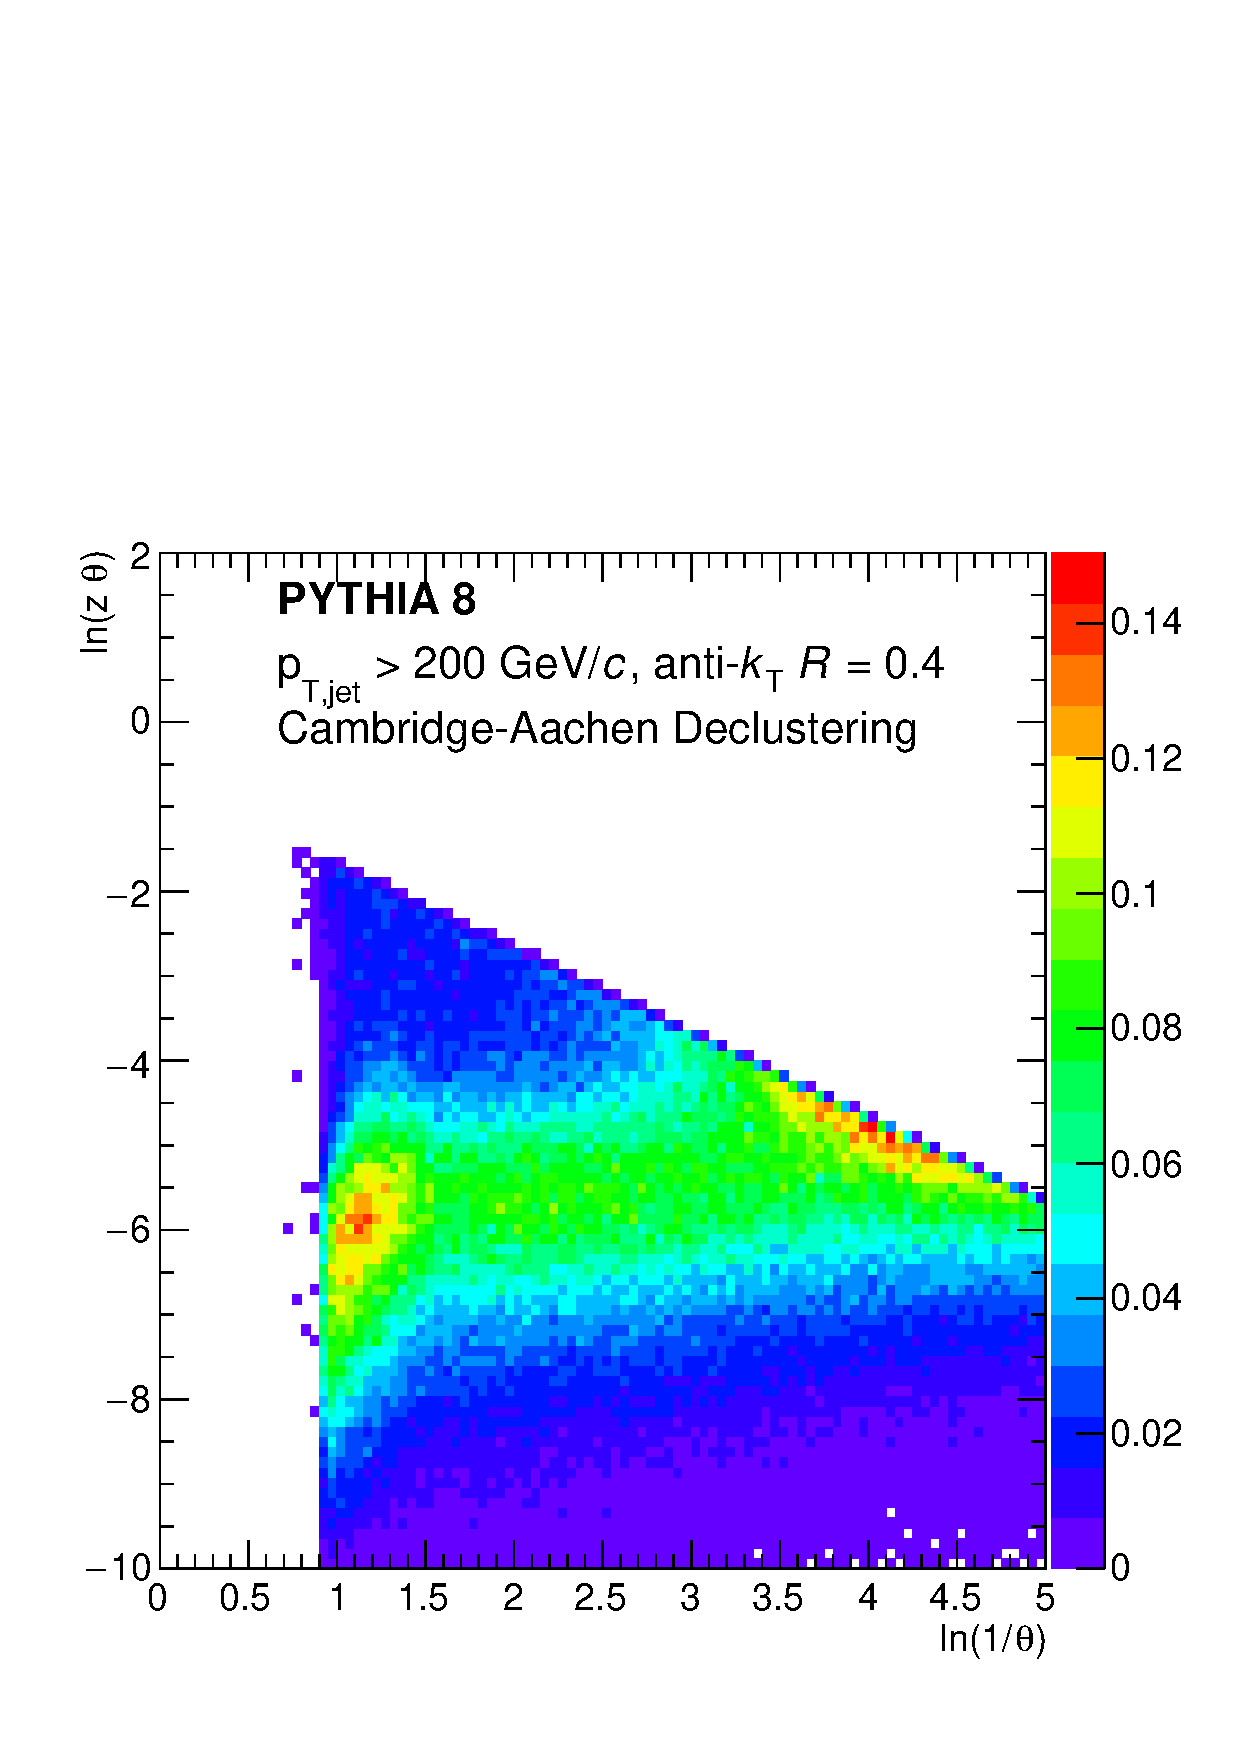
\includegraphics[width=0.33\textwidth]{figures/LundMC/Pythia_CA.pdf}%
%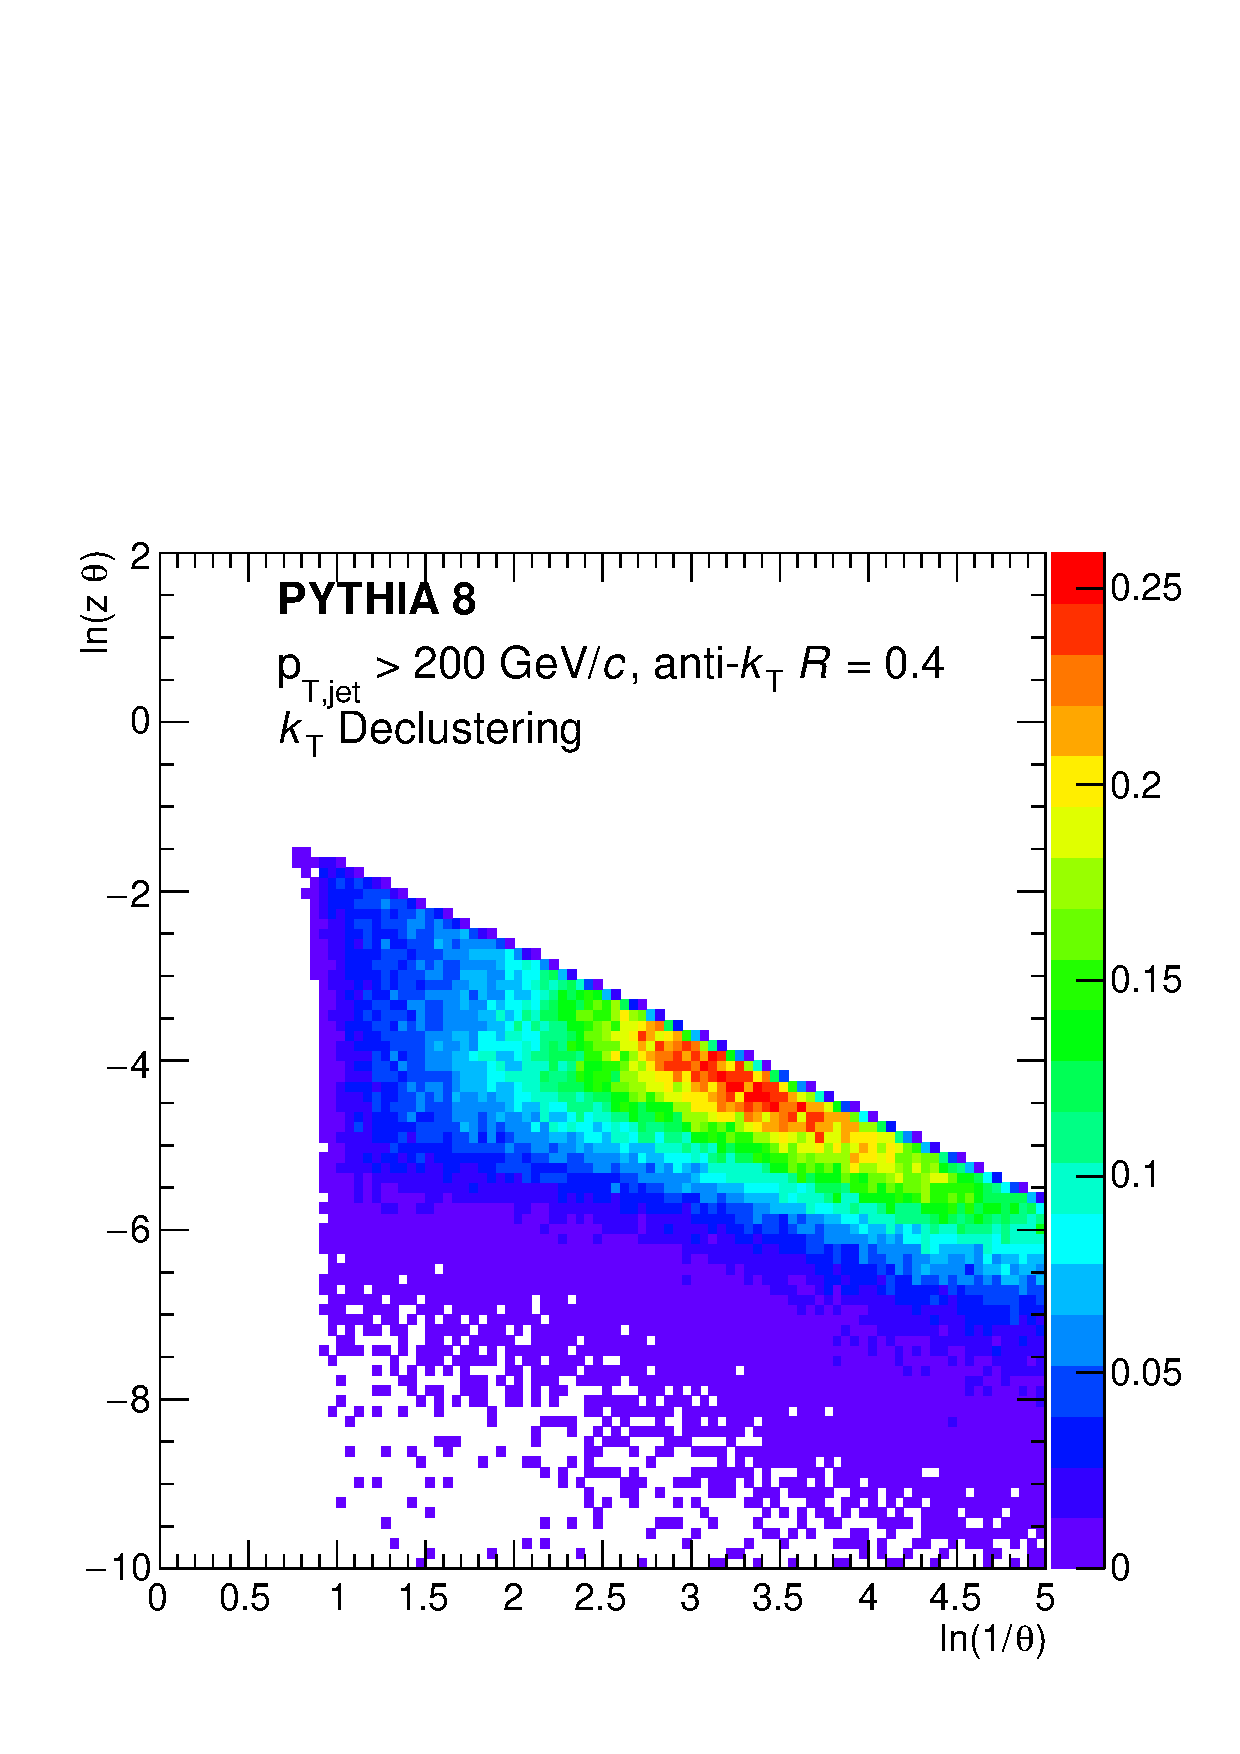
\includegraphics[width=0.33\textwidth]{figures/LundMC/Pythia_kt.pdf}%
%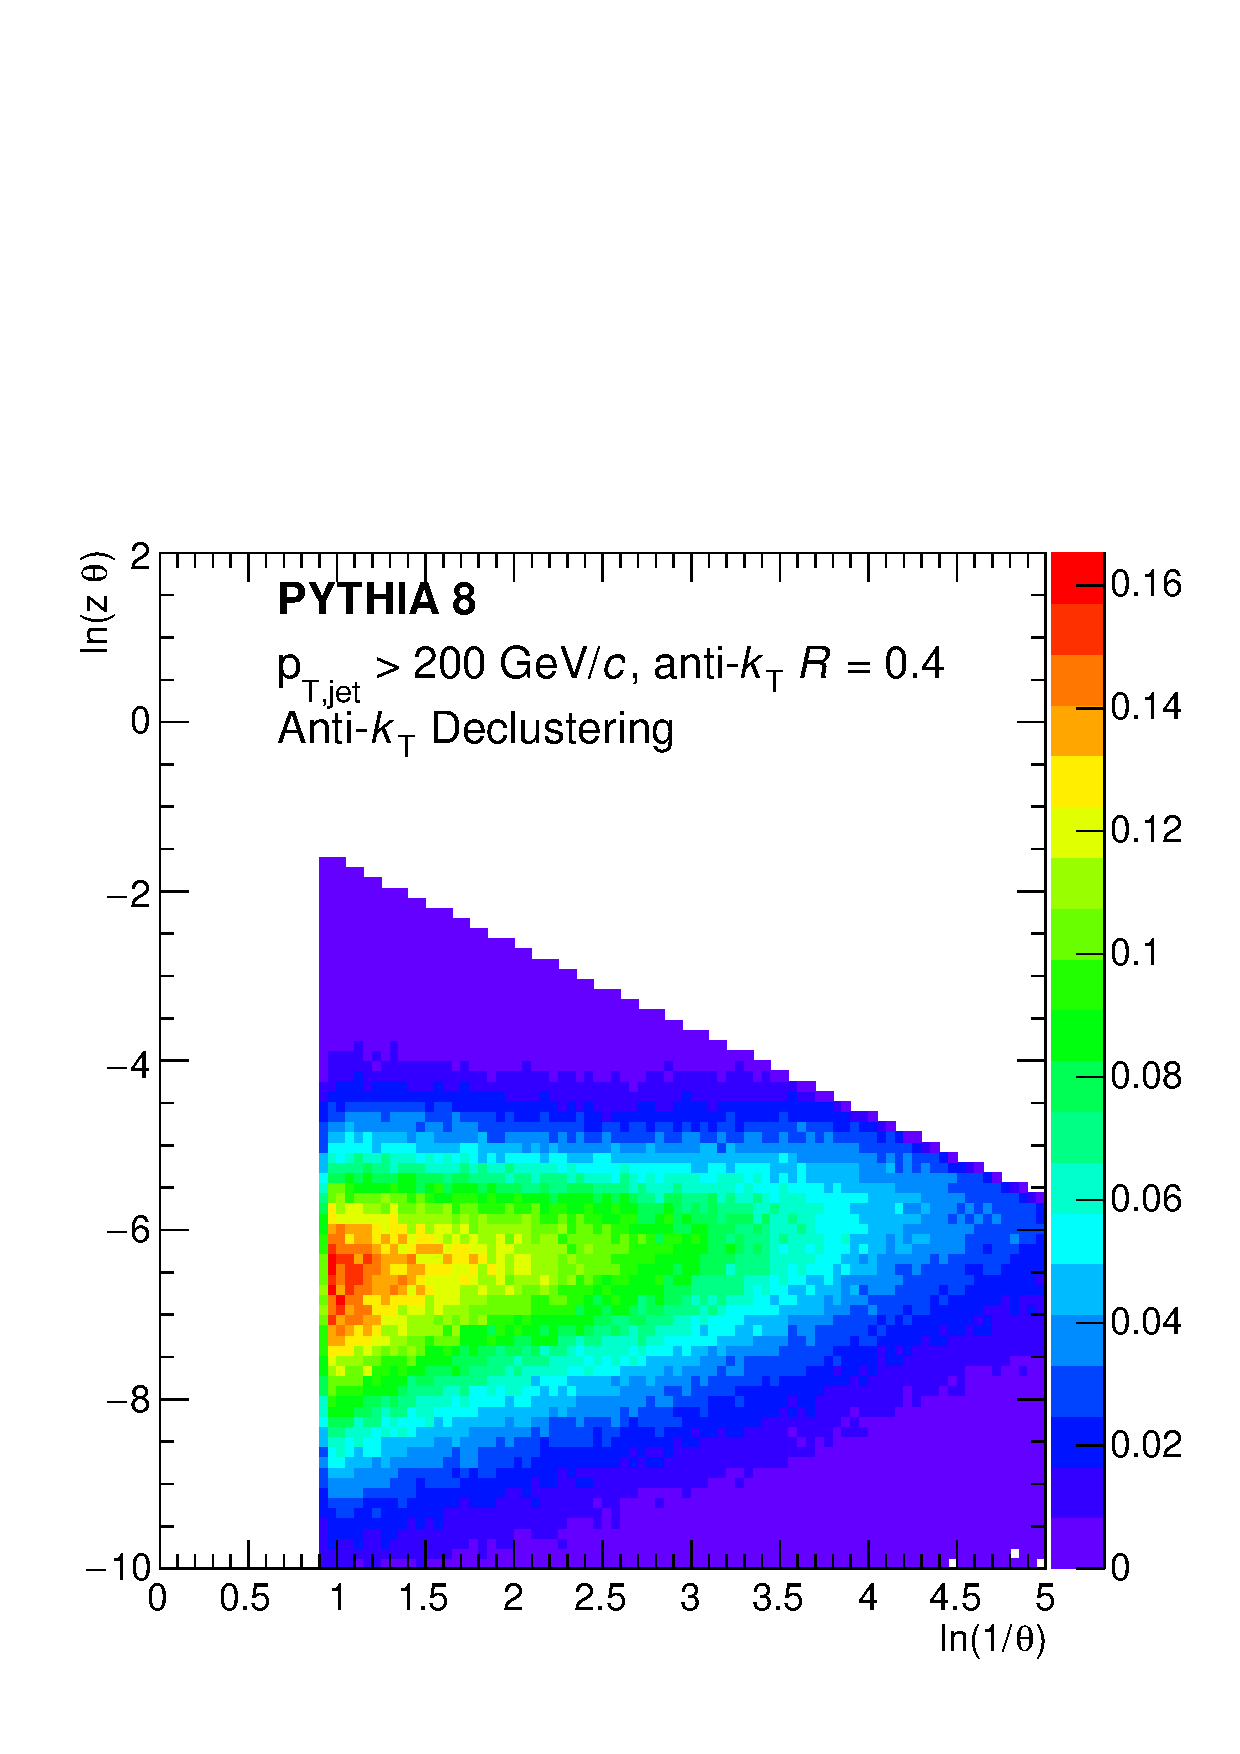
\includegraphics[width=0.33\textwidth]{figures/LundMC/Pythia_Akt.pdf}%
%\caption{Lund plot for different declustering strategies: CA (left), k$_{T}$(middle), Anti-k$_{T}$ (right)}
%\label{fig:AlgoDependence}
%\end{figure}
%
%
%In Fig. \ref{fig:AlgoDependenceSignal}, left plot, the difference between JEWEL (recoils off) and vacuum is shown for k$_{T}$ declustering strategy. The similar plot for QPYTHIA is shown on the right plot. We see that in the case of JEWEL, the excess of splittings at large angle is of the same order of magnitude with CA and k$_{T}$ strategies and around 20 $\%$. In the case of QPYTHIA, the excess of splittings at large $k_{T}$ is enhanced to 20$\%$ with k$_{T}$ strategy compared to the 8$\%$ enhancement we observe for CA strategy in Fig. \ref{fig:PS2Vac} lower left plot. 
%
%
%\begin{figure}[th]
%\centering
%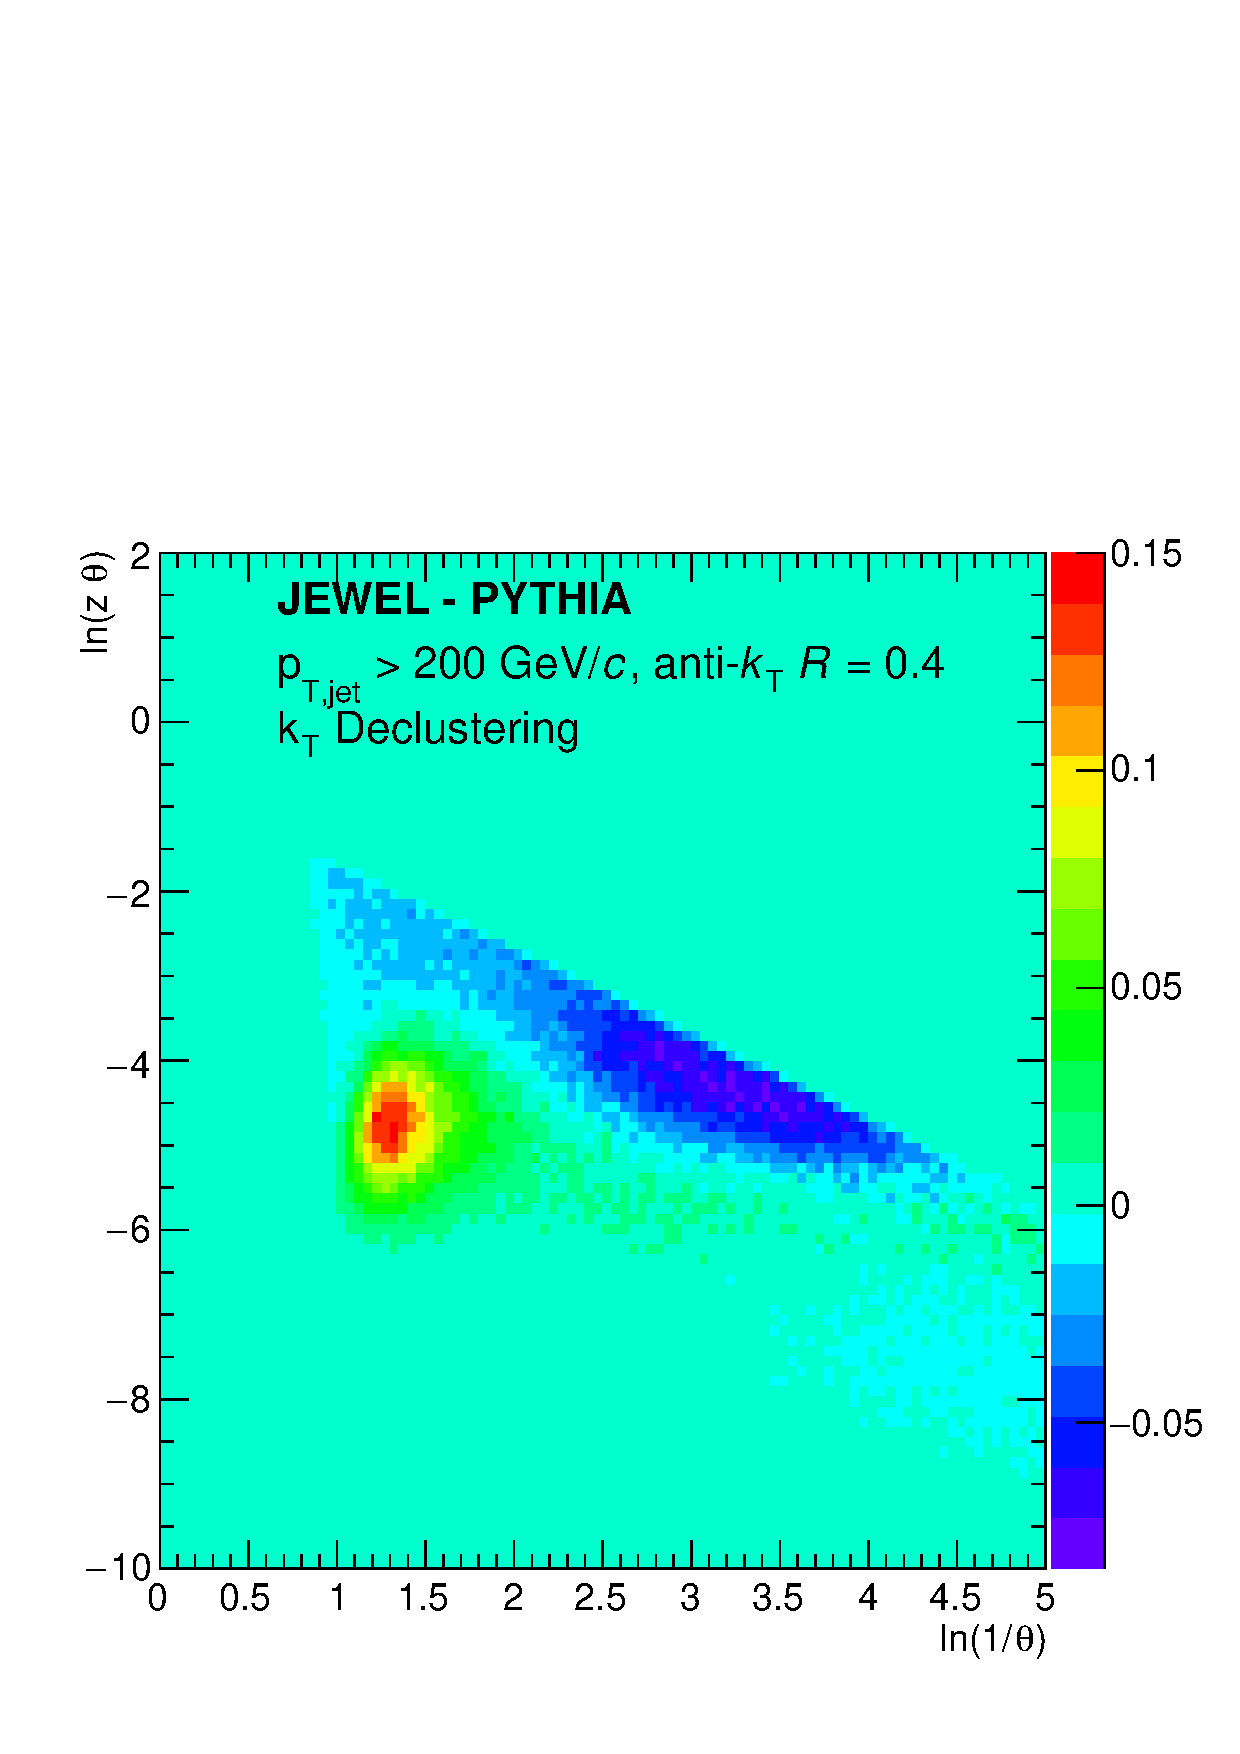
\includegraphics[width=0.33\textwidth]{figures/LundMC/SignalGeneratorDiff_kt.pdf}%
%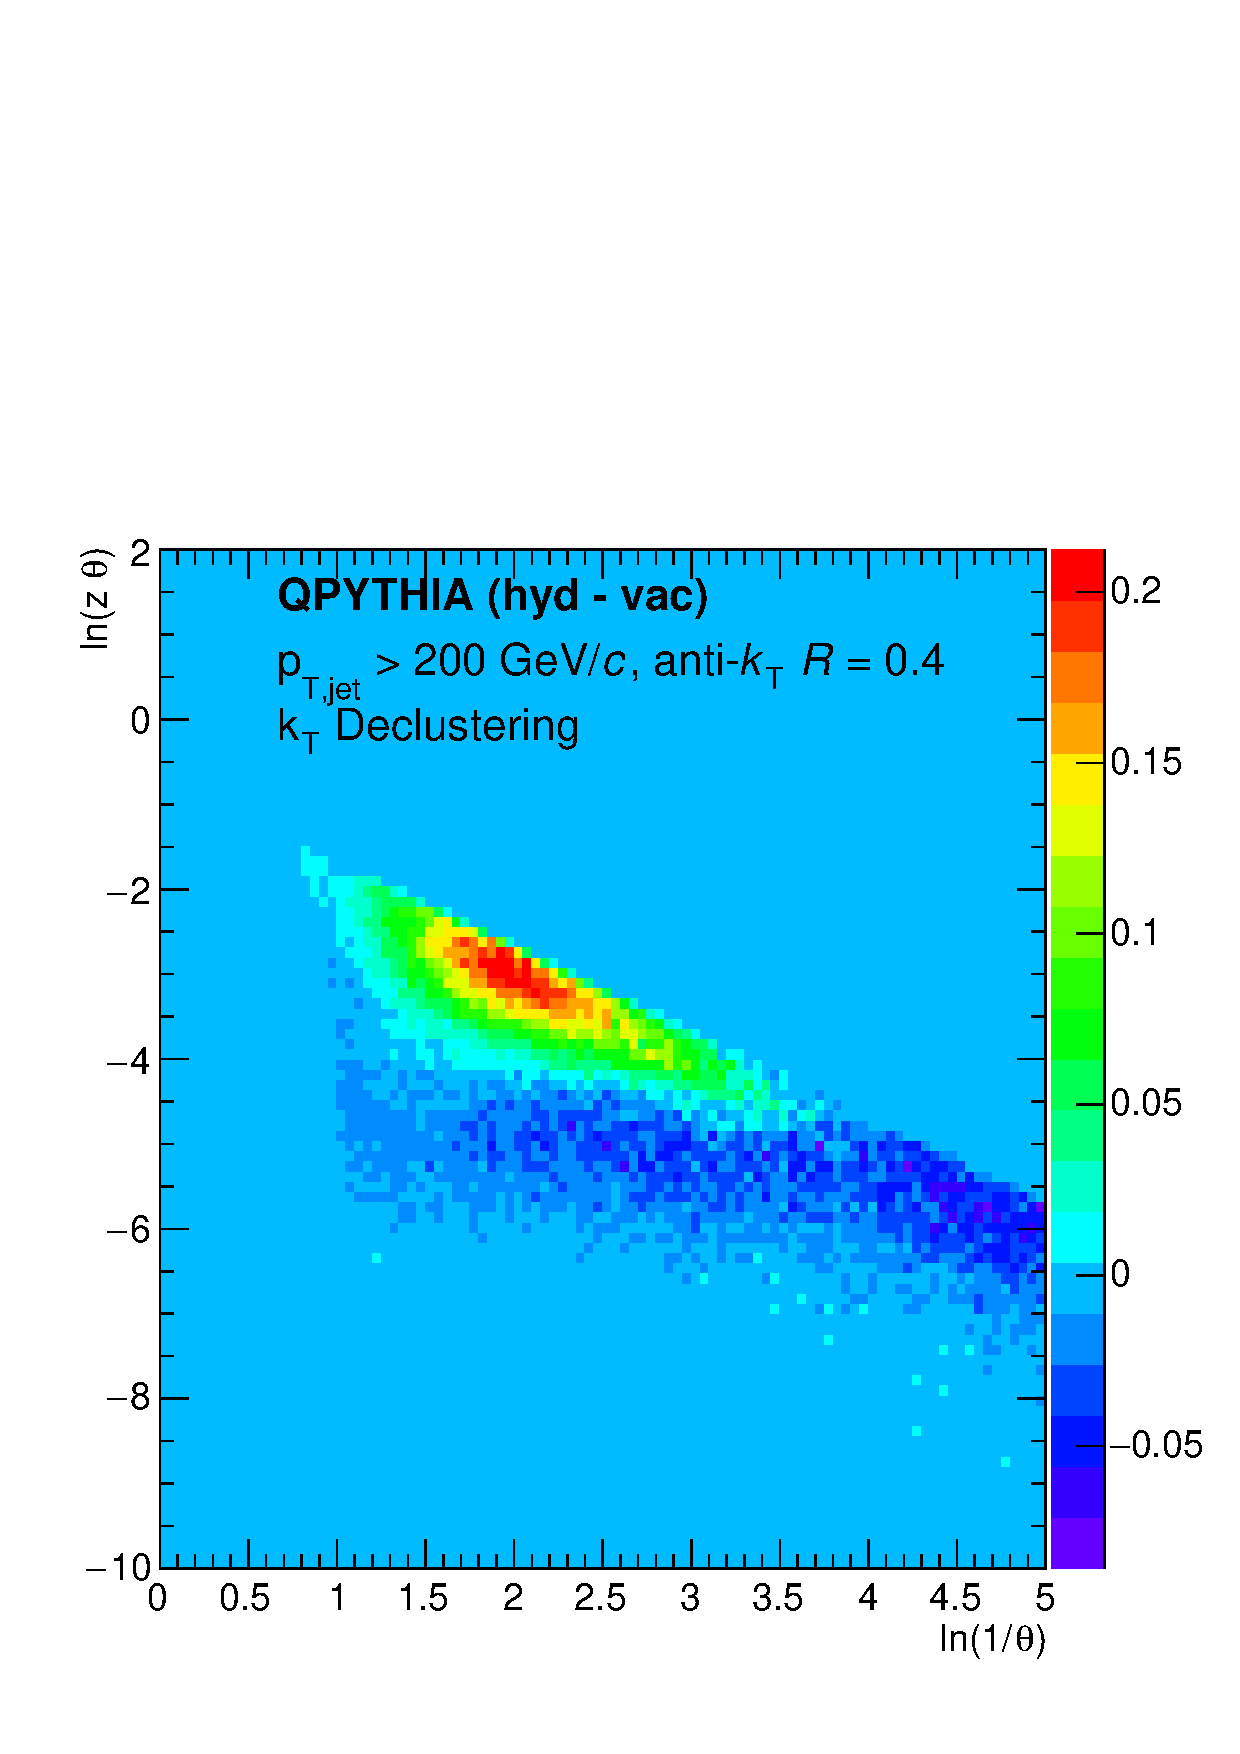
\includegraphics[width=0.33\textwidth]{figures/LundMC/QPythiaDiff_kt.pdf}%
%\caption{Difference of radiation pattern of JEWEL (no recoils) relative to vacuum using k$_{T}$ strategy (left). Same plot for QPYTHIA (right)}
%\label{fig:AlgoDependenceSignal}
%\end{figure}
%
%
%%%%%%%%%%%%%%%%%%%%%%%%%%%%%%%%%%%%%%%%%
\subsubsection{Sensitivity to hadronization effects}
\label{sec:hadronization}
%%%%%%%%%%%%%%%%%%%%%%%%%%%%%%%%%%%%%%%%%


The last stage of the jet fragmentation is the non-perturbative process of hadronization. This is a dynamical process that converts colored partons into color-singlet hadrons. In jet quenching event generators it is typically assumed that hadronization occurs outside of the medium. A proof for this assumption does not exist and therefore hadronization uncertainties should be expected to be sizable. 

%%%%%%%%%%%%%%%%%%%%%%%%%%%%%%%%%%%%%
\begin{figure}[th]
\centering
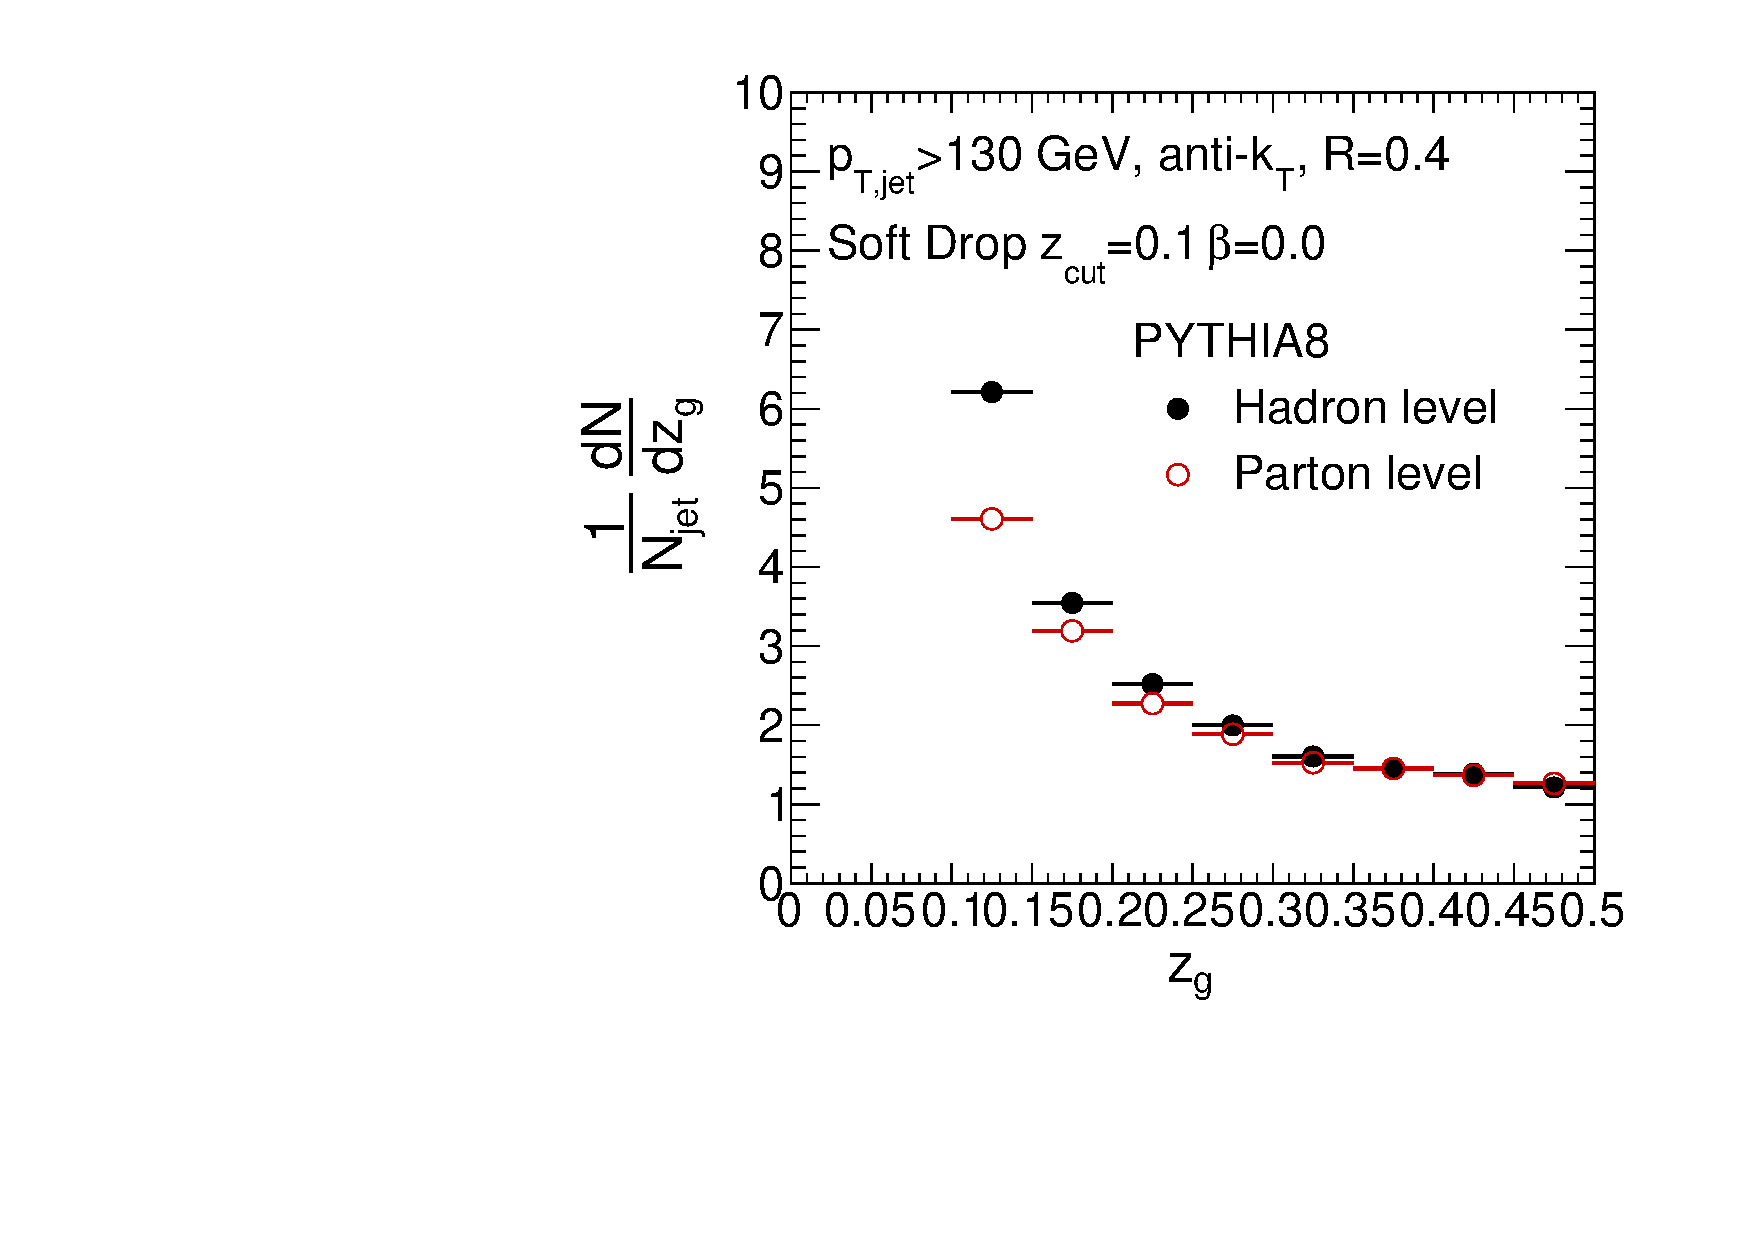
\includegraphics[width=0.33\textwidth]{figures/SDGen/ZgPytHadVsPartBeta00Z01.pdf}%
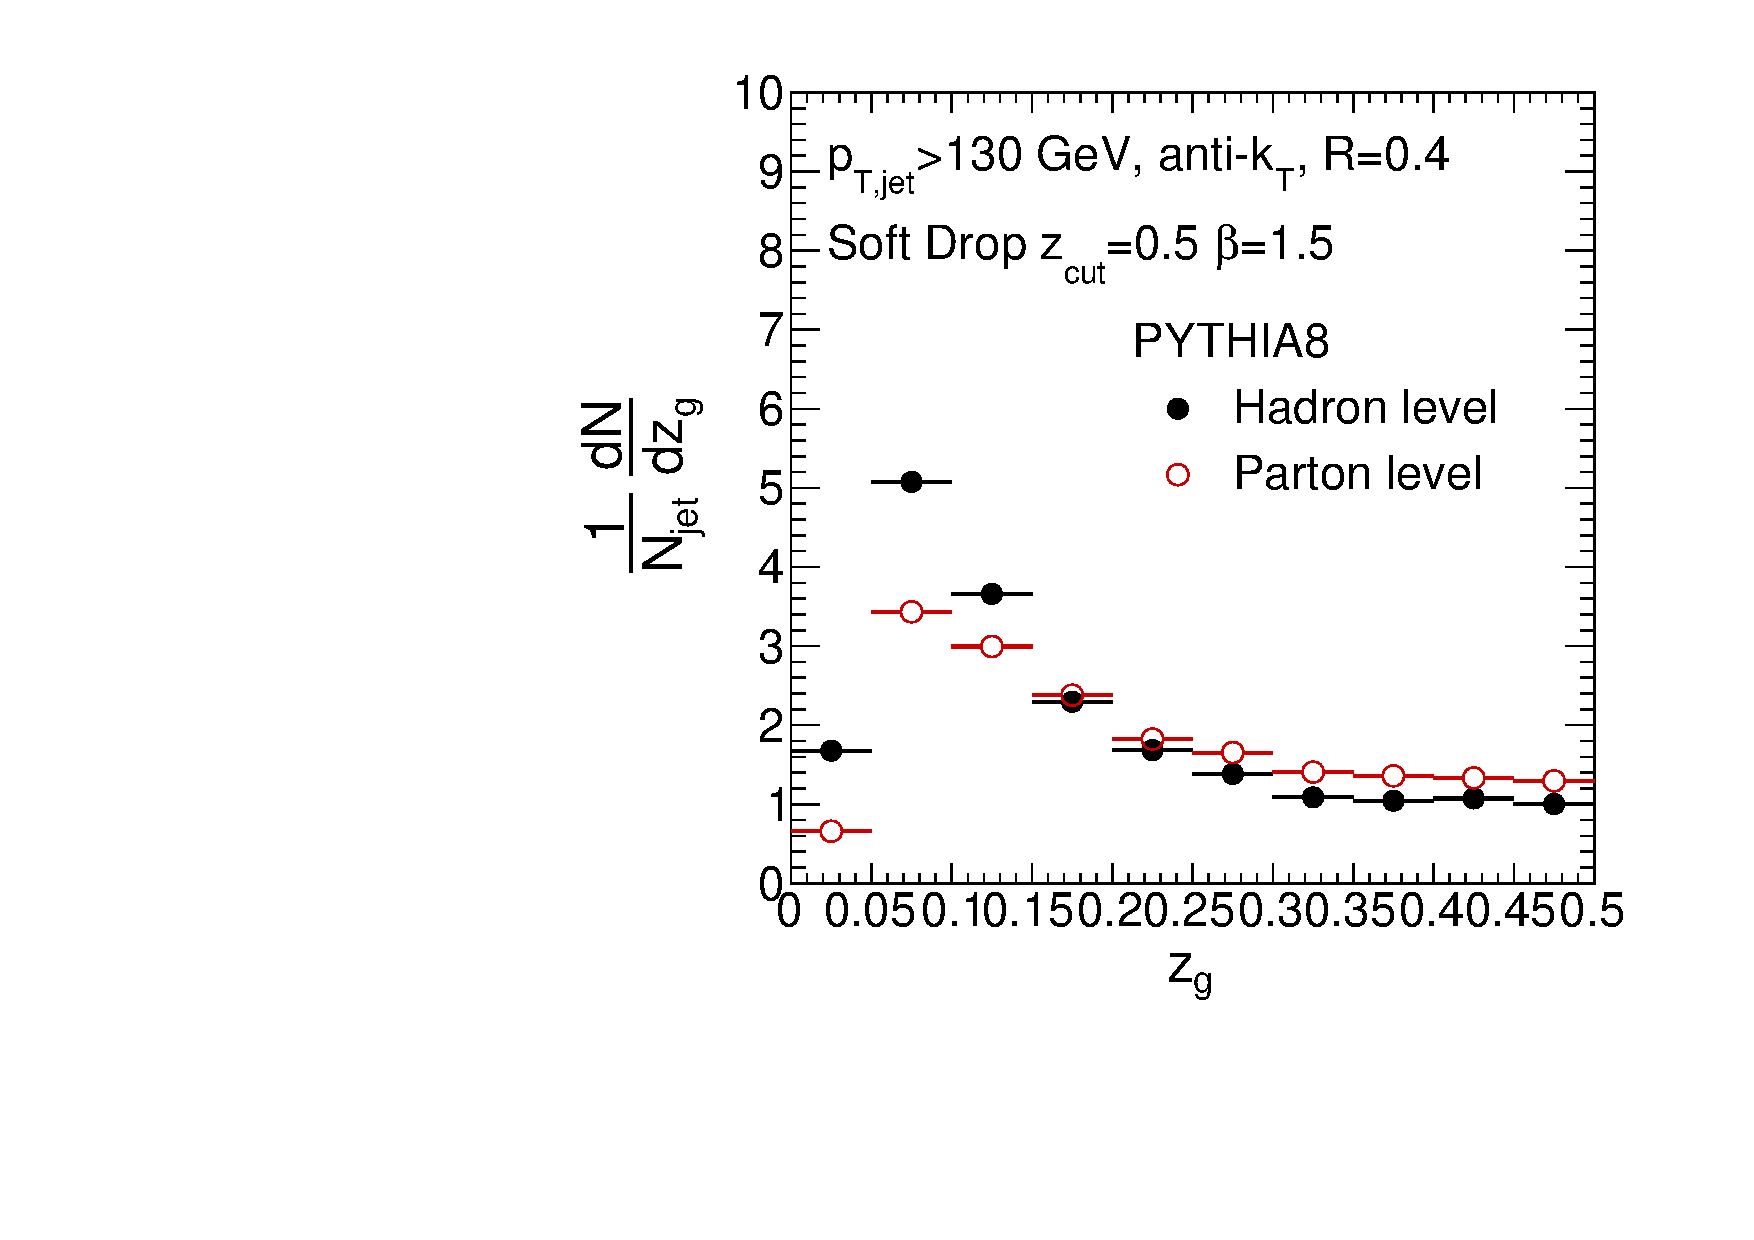
\includegraphics[width=0.33\textwidth]{figures/SDGen/ZgPytHadVsPartBeta15Z05.pdf}%
\includegraphics[width=0.33\textwidth]{figures/SDGen/ZgPytHadVsPartBetam1Z01.pdf}%
\caption{Groomed shared momentum fraction, $z_{\mathrm{g}}$, for three different grooming settings in simulations with and without hadronization with the PYTHIA8 event generator.}
\label{fig:SDGenZGHadVsPart}
\end{figure}
%%%%%%%%%%%%%%%%%%%%%%%%%%%%%%%%%%%%%
Even for vacuum physics, it is well known that the SD procedure has some sensitivity to hadronization effects, for $\beta = 0$ see \cite{Dasgupta:2015yua}.
From perturbative arguments hadronization corrections to the jet $p_{T}$ grow like $R^{-1}$ \cite{Dasgupta:2007wa} and
%inversely proportional to the jet resolution $R$: $\Delta p_{T}^{had} \approx \frac{-1}{R}$, 
so are potentially important for subjet observables.
However, since hadronization is a process that happens locally in phase space, jets are less sensitive to the hadronization uncertainties than observables based on hadrons. In this paragraph we investigate how sensitive groomed subjet observables are to the hadronization process. For this purpose we compare the \zg~distribution in PYTHIA8 with and without hadronization for the three SD settings described above, as shown in \autoref{fig:SDGenZGHadVsPart}. It can be observed that the low-\zg\, region is particularly sensitive to hadronization effects. For grooming with negative $\beta$ the hadron- and parton-level results are most similar, see Fig,~\ref{fig:SDGenZGHadVsPart} (right), because with these grooming settings the soft splittings are rejected. Dedicated studies of these effects in conjunction with medium-modified hadronization are left for the future.

%%%%%%%%%%%%%%%%%%%%%%%%%%%%%%%%%%%%%%%%%
\subsubsection{Issues with changing reclustering algorithm}
\label{sec:reclusteringalgo}
%%%%%%%%%%%%%%%%%%%%%%%%%%%%%%%%%%%%%%%%%

%%%%%%%%%%%%%%%%%%%%%%%%%%%%%%%%%%%%%
\begin{figure}[t!]
\centering
\includegraphics[width=0.4\textwidth]{figures/SDAlgorithms/ndropClusteringComp.pdf}%
\includegraphics[width=0.4\textwidth]{figures/SDAlgorithms/ptratioClusteringComp.pdf}%
\caption{Effects of grooming on trees that are built up using different reclustering algorithms. Left plot: number of grooming steps. Right plot: ratio of jet $\pT$ before and after grooming.
}
\label{fig:PS2Vac_2}
\end{figure}
%%%%%%%%%%%%%%%%%%%%%%%%%%%%%%%%%%%%%
The change of algorithm also strongly affects what happens to the jet after grooming. In \autoref{fig:PS2Vac_2} (left), we show the distribution of the number of grooming steps for the three reconstruction algorithms discussed above. In particular, we note that the $k_\perp$ and the anti-$k_\perp$ algorithms result in completely different grooming. While the jet reconstructed with the former algorithm are mainly unaffected by grooming, in the latter case of the order of $\sim 10-20$ branches are groomed away. This also strongly affects the $\pT$ of the groomed jet, as seen in \autoref{fig:PS2Vac_2} (right), where the groomed jets in the anti-$\kT$ sample on average lose $\sim 20$\% of their energy. The C/A algorithm falls in between the two extremes, and is the only algorithm that maps the phase space with an approximately constant density, see \autoref{fig:PS2Vac} (left). Of the order of $\sim 5$ branches are removed by the grooming procedure on average, which slightly reduces the jet $\pT$ by $\lesssim 10$\%.

%%%%%%%%%%%%%%%%%%%%%%%%%%%%%%%%%%%%%
\begin{figure}[th]
\centering
\includegraphics[width=0.32\textwidth]
{figures/SDAlgorithms/zgClusteringComp.pdf}
\includegraphics[width=0.32\textwidth]
{figures/SDAlgorithms/rgClusteringComp.pdf}
\includegraphics[width=0.32\textwidth]
{figures/SDAlgorithms/mgClusteringComp.pdf}%
\caption{Subset of grooming variables, symmetry parameter ($z_{g}$), groomed mass ($M_{g}$) and groomed radius ($\Delta R_{12}$) for three different jet reclustering algorithms.}
\label{fig:SDClusteringComp}
\end{figure}
%%%%%%%%%%%%%%%%%%%%%%%%%%%%%%%%%%%%%
Finally, we studied the behavior of the three observables subject to different reclustering algorithms applied, see \autoref{fig:SDClusteringComp}. In this particular case, we limit ourselves only to looking at the PYTHIA8 (vacuum) samples.
In case of a grooming prescription that requires a semi-hard splitting, for instance like in the SD1 setting,
%$z_{cut}$=0.1, $\beta=0$, 
the number of groomed branches will be large for anti-$k_{\rm \tiny T}$ reclustering ($\lesssim 30$) and very small for $k_{\rm \tiny T}$, for which the grooming conditions will be satisfied at the first iteration in most of the cases. Consistently, the groomed momentum fraction \zg\, probes very asymmetric splittings in the case of anti-$k_{\rm \tiny T}$ reclustering as can be seen in \autoref{fig:SDClusteringComp} (left). In contrast, $k_{\rm \tiny T}$-reclustered \zg\, picks exclusively up symmetric splittings, resulting in an almost featureless distribution. Similar conclusions can be made for the $\Delta R_{12}$ distribution, \autoref{fig:SDClusteringComp} (center), and $M_g$, \autoref{fig:SDClusteringComp} (right), as well. These artifacts are hard to reconcile with the expected behavior from QCD theory, and will therefore generally not be pursued further.


%%%%%%%%%%%%%%%%%%%%%%%%%%%%%%%%%%%%%%%%
\subsection{Enhancing jet quenching observables using grooming}
\label{sec:dissecting}
%%%%%%%%%%%%%%%%%%%%%%%%%%%%%%%%%%%%%%%%

Many jet quenching observables, such as the nuclear modification factor $R_{AA}$ and the momentum imbalance in photon-jet events, are considered benchmark measurements that quantify the amount of in-medium energy-loss and broadening. For reviews, see e.g. \cite{dEnterria:2009xfs,Majumder:2010qh}. However, their constraining power to discriminate between models have also been questioned. In some cases, the influence of background fluctuations can further obscure their constraining power.

In this section we present studies of conventional jet quenching observables that are enhanced by using grooming techniques.  As a first step, we apply SD grooming on the inclusive jet sample, extracting from each jet the grooming variables $z_g$ and $\Delta R_{12}$. 
This allows to further sub-divide the sample according to a measure involving these variables. 
For the purposes of this report, we have simply binned the fully inclusive sample according to the angle separating the two hardest subjets of a particular jet. This is motivated by the studies using splitting maps and the results obtained for the substructure observables previously. Another motivation is to differentiate between the modifications of the ``soft'' and the ``hard'' structure of the jet. The former is more dominant for inclusive observables and for non-restrictive SD settings, e.g. SD1 and SD2 in \autoref{fig:TheorySD} (left and central panels), while the latter would be more pronounced for conservative SD parameter choices, such as SD3 in \autoref{fig:TheorySD} (right panel).

Due to the limited scope of the workshop, we have not attempted to study this in any systematic way. Here, we only report on the two following studies at LHC energies:
\begin{itemize} 

\item the nuclear modification factor $R_{AA}$ binned in the angular separation $\Delta R_{12}$ as found with SD2.

\item the $x_{J\gamma}$ distribution binned in the angular separation $\Delta R_{12}$ as found with SD1. 
\end{itemize}
For both grooming settings, comparing small- and large-angle substructure configurations also gives an additional handle on the formation time of that particular splitting, see \autoref{fig:PS0} (right).

In both cases, jets were reclustered and groomed, and only jets that had a candidate subjet pair that fulfilled the Soft Drop condition were further analyzed.
More importantly, all results in this section have been computed by embedding the MC jet samples into a realistic, centrality-dependent heavy-ion background, for details see \kmt{where?}. Therefore, these result reflect more realistically the magnitude of effects that should be expected to arise in heavy-ion collisions at the LHC.
%{\color{red} Are the curves for $\Delta R>0.3$ consistent with the expected effect of uncorrelated background at large angles...? Was additional pile-up mitigation employed?}

The well-known nuclear modification factor $R_{AA}$ compares the yields of equivalent hard processes in heavy-ions and proton-proton collisions, and is given schematically as
\beq
\label{eq:RAA}
R_{AA} = \frac{\dd N_{AA}/\dd \pT^2 \dd y}{\langle N_\text{coll} \rangle \dd N_{pp}/\dd \pT^2 \dd y} \,,
\eeq
where $\langle N_\text{coll} \rangle$ counts the number of nucleon-nucleon collisions in a given centrality range,
is a standard benchmark for estimating/tuning medium parameters in theoretical calculations and Monte Carlo jet quenching models. By dividing the sample of inclusive high-$\pT$ jets into small- and large-angle configurations, we obtain more differential information regarding the accompanying modifications of the intra-jet structure. Similar studies, albeit using another method to dissect the jet sample into two-prong structures, was already presented in \cite{Zhang:2015trf,Apolinario:2017qay}.
Note, however, that the suggested ``binning'' procedure could be sensitive to different physical mechanisms separately in the proton-proton and heavy-ion events. Disentangling this would demand further studies.

%%%%%%%%%%%%%%%%%%%%%%%%%%%%%%%%%%%%%
\begin{figure}[th]
\centering
\includegraphics[width=0.32\textwidth]{figures/Observables_RAA/Plot9}
\includegraphics[width=0.32\textwidth]{figures/Observables_RAA/Plot3}
\includegraphics[width=0.32\textwidth]{figures/Observables_RAA/Plot4}
%\includegraphics[width=0.33\textwidth]{figures/LundMC/PythiaDiffCA_wLines200.pdf}%
%\includegraphics[width=0.33\textwidth]{figures/LundMC/PythiaDiffCA_wLines80120.pdf}%
\caption{The nuclear modification factor for subsamples of jets that have been unrolled as a function of $\Delta R$ of the leading sub-jets identified using SD1. 
}
\label{fig:GroomedRAA}
\end{figure}
%%%%%%%%%%%%%%%%%%%%%%%%%%%%%%%%%%%%%
The jet samples generated from QPYTHIA, JEWEL ``Recoil off'' and JEWEL ``Recoil on'' that goes into calculating $R_{AA}$ in \autoref{fig:GroomedRAA}, has been binned according to the angular separation of the subjets identified using SD3 grooming, $\Delta R_{12}$. While all three models show a similar transverse momentum dependence of $R_{AA}$ for the fully inclusive sample (see black points in \autoref{fig:GroomedRAA}), large differences are seen for the more differential  results.\footnote{The overall magnitude of the inclusive $R_{AA}$ does not play an important role for the point we are trying to make here.} 

In QPYTHIA, the core of the jet is quenched stronger than the periphery, as expected from previous studies above, see \autoref{fig:GroomedRAA} (left). It is basically related to the enhanced splitting of collinear modes. For the JEWEL ``Recoils off'' sample, see \autoref{fig:GroomedRAA} (center), the effect is completely opposite: the jet core is quenched much less than large-angle configurations. This also comes as no surprise in light  of other substructure observables that were analyzed above, see e.g. \autoref{sec:groomedobservables}, and reflects stronger energy-loss effects for large-angle substructure fluctuations which implies that more partons are quenched \cite{Milhano:2015mng}. Finally including recoil effects, the JEWEL ``Recoils on'' sample, see \autoref{fig:GroomedRAA} (right), reveal a strong $\pT$-dependence of large-angle jets, leading to a big enhancement of $R_{AA}$ at relatively low transverse momenta. This implies of an enhanced constraining power to details of medium recoil modeling in this observable.

Other benchmark observable in heavy-ion collisions include the $Z$-jet or photon-jet momentum asymmetry. Here, we will only focus on the latter.
We recall that the variable $x_{J\gamma}$ is defined as the ratio of jet to photon momentum, 
\beq
x_{J\gamma} = \frac{p_\text{{\tiny T},jet}}{p_{\text{\tiny T},\gamma}} \,.
\eeq
In contrast to the nuclear modification factor \eqref{eq:RAA}, this observable does not immediately involve a comparison to a proton-proton baseline. The direct access to the photon energy in the measurement also would help constrain the effect of energy-loss or migration of jets between $\pT$-bins.

%%%%%%%%%%%%%%%%%%%%%%%%%%%%%%%%%%%%%
\begin{figure}[th]
\centering
%\includegraphics[width=0.5\textwidth]
%{figures/Observables_GammaJet/GammaJet_groomed}%
\includegraphics[width=0.5\textwidth]
{figures/Observables_GammaJet/JEWEL-photon-jet-recoilOn-linear}%
\caption{The $x_{J\gamma}$ distribution for subsamples of jets that have been unrolled as a function of the angle found between the leading sub-jets using SD. }
\label{fig:GroomedGammaJet}
\end{figure}
%%%%%%%%%%%%%%%%%%%%%%%%%%%%%%%%%%%%%
In \autoref{fig:GroomedGammaJet} we present the resulting $x_{J\gamma}$ distribution for the JEWEL ``Recoils on'' samples in two centrality bins (corresponding to $0-10$\% and $90-100$\% centrality). This sample has been binned in subjet angular separation, as described above, this time using SD2 grooming. The same features that have been pointed out multiple times, also show up here as a function of collision centrality. Notably, the small-angle sample shows very little dependence of centrality, and is closely peaked around 1. The large-angle sample, on the other hand, which also corresponds to jets formed earlier in the medium, is strongly distorted. While the distribution for  90-100\% centrality is broader for the large-angle sample, we observe that the peak structure, which is clearly visible in \autoref{fig:GroomedGammaJet}), is completely removed when going to the most central collisions. 
%\kmt{Features: groomed substructure gives us access to binning in formation time of that splitting of substructures; large angle sample is strongly modified! Very constraining for recoil modeling..? No need for pp baseline (often binning in ``heavy-ion-modified'' variables sample completely different processes in pp and AA. }
\kmt{Can we get a result for QPYTHIA?}

These proof-of-principle studies illustrate the enhanced sensitivity to more than one variable that can be obtained by differentiating the inclusive jet sample using a well-controlled procedures. 
In this section, we have analyzed medium-modified jet samples embedded in a heavy-ion background and utilized the angular separation between the leading subjets, as extracted Soft Drop procedure, in order to bin the jets into small- and large-angle configurations. While this should not come as a surprise in light of the previous results on the groomed substructure observables $z_g$, $\Delta R_{12}$ and $M_g/\pT$, we observe very different modification patters between the employed models and potentially large effects. Measurements of jets recoiling from $Z$-bosons or photons could prove as especially valuable in tracking how jets are modified in all variables, including the overall $\pT$ shift.
However, the results presented in this section are only exploratory and more systematic studies are left for the future.

%!TEX root = THinstituteReport_1.tex

%%%%%%%%%%%%%%%%%%%%%%%%%%%%%%%%%%%%%%%%
\section{Outlook}
\label{sec:outlook}
%%%%%%%%%%%%%%%%%%%%%%%%%%%%%%%%%%%%%%%%

The investigation of QCD jet observables in heavy-ion collisions is a community-wise effort, involving both experimentalists and theorists. 
While significant progress, both from the point of view of the development of experimental techniques as well as from theoretically founded parametric estimates grounded on scale analysis and modeling within Monte-Carlo parton showers, has led to a quite detailed qualitative \textsl{general} understanding of how jets are modified in the medium created in the aftermath of heavy-ion collisions, the field has not reached the level of precision associated with jet measurements in other colliding systems, such as proton-proton and DIS.
It is therefore worth considering whether it be possible and fruitful to contemplate strategies that would be useful to further enhance jet observables as unique and valuable probes of the quark-gluon plasma.
%consolidate measurements with first-principle theory in order to establish well-controlled baselines across jet samples and observables. 
A first attempt at such an ambitious step would be to find a common language within the field of heavy-ions for comparisons between experimental data and theory. However, it is almost as important to develop common ground with the wider field of high-energy physics, based on the language of perturbative QCD and the tools of modern high-energy experiments.

\kmt{Suggestions for future studies.}

The ``Novel tools and observables for jet physics in heavy-ion collisions'' workshop provided an opportunity to work toward this goal.
%comparisons between various implementations of jet quenching modeling. The Lund kinematical diagram provides an eagle's view of the branching process as implemented in a particular code, avoiding the model details that often distract from seeing the big picture.
The concrete calculations and model studies presented in this report can, of course, be further scrutinized and improved. However, the main messages could be relevant for the field at large. Let us summarize in two points.
\begin{itemize}

\item We have introduced a operational way to map the full content of a jet splitting process, making use of the Lund diagram. Using kinematical arguments, we can make sense of enriched and depleted regions of phase space as results of medium interactions and recoil. An important caveat is that this idealized picture gets strongly distorted due to the presence of uncorrelated background but we have shown, through various exercises, that this aspect mostly affects the low-$\pT$ observables.

\item We have outlined a strategy to single out jet samples enriched in configurations possessing specific properties as an aid to single out physics mechanisms, in particular \textsl{hard} (e.g. medium-induced bremsstrahlung, modifications of intra-jet structure due to energy loss) from \textsl{soft} (e.g. particle yield, sensitivity to recoil) medium effects and, similarly, \textsl{large-angle} from \textsl{small-angle} components.

\end{itemize}
We hope the topics we have reported here would trigger new and exciting future studies of jet, and in particular jet substructure, observables in heavy-ion collisions.



\section*{Acknowledgements} 
We thank the CERN TH department for hosting and supporting the organization of the 5th Heavy Ion Workshop and the TH institute ``Novel tools and observables for jet physics in heavy-ion collisions'' and especially Michelangelo Mangano and Angela Ricci for providing organizational support before and during the meeting.

\appendix
%!TEX root = THinstituteReport_1.tex

%%%%%%%%%%%%%%%%%%%%%%%%%%%%%%%%%%%%%%%%%%
\section{Monte-Carlo parton showers}
\label{app:models}
%%%%%%%%%%%%%%%%%%%%%%%%%%%%%%%%%%%%%%%%%%

This section briefly outlines the main physics ingredients of the MC in-medium parton shower generators used in course of the workshop. For detailed descriptions, we refer the interested reader to the original references.

%%%%%%%%%%%%%%%%%%%%%%%%%%%%%%%%%%%%%%%%%%
\subsection{QPYTHIA}
\label{app:qpythia}
%%%%%%%%%%%%%%%%%%%%%%%%%%%%%%%%%%%%%%%%%%

This appendix provides some details of the implementation of medium effects on the final-state parton shower as implemented in QPYTHIA \cite{Armesto:2009fj}. As the name suggests, the program builds on PYTHIA6 \cite{Sjostrand:2007gs,Sjostrand:2008vc}. The final-state shower is a mass-ordered (or virtuality-ordered) shower, where the Sudakov form factor is defined as
\beq
\label{eq:QPYTHIASudakov}
\Delta(t_1,t_0) = \exp\left[\int_{t_0}^{t_1} \frac{\dd t}{t} \int_{z_-}^{z^+} \dd z \, \frac{\alpha_s(t)}{2\pi}P(z)\right] \,,
\eeq
where the limits $z_\pm = z_\pm(t)$ implement the perturbative constraints and the evolution variable $t = M^2$ is the (squared )virtuality or invariant mass, see Eq.~\eqref{eq:DipoleMass}. The quantity in Eq.~\eqref{eq:QPYTHIASudakov} represents the probability of no splitting between the mass-scales $t_0$ and $t_1$ and can be used to determine the variables $(z,t)$ of the subsequent splitting in the shower by a standard dicing procedure. Although the shower is ordered in mass, angular ordering is enforced by a veto procedure.

In vacuum, the function $P(z)$ corresponds to the relevant Altarelli-Parisi splitting functions. However, in the medium one takes advantage of the fact that the medium-induced radiative spectrum comes simply in addition to the existing vacuum one \cite{Wang:2001ifa,Polosa:2006hb}, to substitute
\beq
P(z) \to P^\tot(z) = P(z) + \Delta P(z)
\eeq
in Eq.~(\ref{eq:QPYTHIASudakov}), where 
\beq
\Delta P(z) = \frac{2\pi t}{\alpha_s} \frac{\dd I^\med}{ \dd z \dd t} \,,
\eeq
where $\dd I^\med /(\dd z \dd t)$ is identified with the (double-differential) BDMPS spectrum. In the current implementation of QPYTHIA it is computed in the multiple-soft scattering approximation, that neglects hard medium interactions, and in the soft limit $z \ll 1$. In addition, the splitting function $g \to q\bar q$ is not modified by this prescription since it is subleading.

%%%%%%%%%%%%%%%%%%%%%%%%%%%%%%%%%%%%%%%%%%
\subsection{JEWEL}
\label{app:jewel}
%%%%%%%%%%%%%%%%%%%%%%%%%%%%%%%%%%%%%%%%%%

JEWEL is also based on PYTHIA6, and handles exclusively the final-state parton shower routine. Let us summarize the main steps of the modified shower routine in three points.
\begin{itemize}

\item Within the program, every interaction with the medium is treated similarly to the hard, partonic scattering itself and described by a $2 \to 2$ perturbative matrix element, suitably regularized in the IR due to the dressing of medium quasi-particles. Hence, one invokes so-called ``partonic parton densities'' to allow hard medium kicks to resolve additional (virtual) jet constituents in course of the interaction. Scattering with the medium can also give rise to additional radiation.

\item The emission with the shortest formation time is realized first. This allows for a smooth interpolation between so-called vacuum emissions and the ones that are affected by medium interactions, often referred to as ``medium-induced''.

\item The LPM effect is implemented by keeping track of the amount of re-scattering during the formation time of radiation.
\end{itemize}
Comparing to the analytical limits of single-gluon radiation spectrum, this treatment allows to treat the kinematics of emission and the interactions on a more precise level.

In addition to the showering, JEWEL also permits to track the momenta and color flow of the recoiling medium constituents that happen to interact with the jet. Note that the medium parton is counted as a final-state particle directly after the scattering, and is not allowed to interact further. We refer to this mode as ``Recoils on''. The mode ``Recoils off'' refers to the case when these partons are not included in the event record and discarded. In the former case, it is imperative to subtract the thermal momentum of the partons before their interaction with the jet, since it forms part of the uncorrelated  thermal background in heavy-ion events. This is most reliably done with the so-called ``4MomSub'' procedure which consists of subtracting the sum momenta of medium constituents entering a given jet, for further details see \cite{KunnawalkamElayavalli:2017hxo}. 


\bibliographystyle{elsarticle-num}
%\section*{\refname}
\bibliography{THinstituteRefs}

\end{document}

